\documentclass[12pt, a4paper,twoside]{tesi_upf}


%CODIFICATION
\usepackage[latin1]{inputenc}
\usepackage[T1]{fontenc}    % use 8-bit T1 fonts
\usepackage{url} 

%IMPORTED PACKAGES BY GUILLERMO
\usepackage{booktabs}       % professional-quality tables
\usepackage{amsfonts}       % blackboard math symbols
\usepackage{nicefrac}       % compact symbols for 1/2, etc.
\usepackage{microtype}      % microtypography
\usepackage{xcolor}         % colors
\usepackage{mathtools}
\usepackage[noend]{algpseudocode}
\usepackage{amsthm}
\usepackage{adjustbox}
\usepackage{todonotes}
\usepackage{amssymb}
\usepackage{comment}
\usepackage{caption}
\usepackage{subcaption}
\usepackage{xspace}
\usepackage{booktabs}
\usepackage{tabularx}
\usepackage{multirow}
\usepackage{amsmath}
\usepackage{natbib}
\usepackage{tikz}
\usepackage{algorithm}
\usepackage[noend]{algpseudocode}
% \usepackage{mathspec} 
\usepackage{adjustbox}
\usepackage{dsfont}
\usepackage{thmtools}
\usepackage{thm-restate}
\usepackage{setspace}
\usepackage{comment}


\usepackage[hyperfootnotes=false]{hyperref}
\hypersetup{
  citecolor=blue,}


\usetikzlibrary{arrows,automata,positioning}
\usetikzlibrary{shapes.multipart}
\usetikzlibrary{decorations.markings}
\usetikzlibrary{decorations.pathreplacing}

%LENGUAGE
\usepackage[english,catalan]{babel}

%ONLY TO OBTAIN MARK BANK INDEX INDICATION A4
\usepackage[cam,a4,center,frame]{crop}

%INCLUDE GRAPHICS AND THE LOGO OF THE UPF
\usepackage{graphicx}

%FONTS TIMES OR GARAMOND, 
%\usepackage{times}
\usepackage{ebgaramond}

%WITHOUT HEADINGS: NO MODIFICATION
\pagestyle{plain}

%FOR THE INDEX OF SUBJECTS
\usepackage{makeidx}
\makeindex


\usepackage{enumitem}
\setlist[itemize]{topsep=-0.5pt}

\usepackage{rotating}

%SELECT LANGUAGE
\selectlanguage{english}

%THE TABLE OF CONTENTS IS TITLE CONTENTS
\addto\captionscatalan
  {\renewcommand{\contentsname}{\Large \sffamily Sumari}}


%COMMANDS CREATED BY GUILLERMO

\DeclareMathOperator*{\argmax}{arg\,max}

% macros:
\newcommand{\tS}{\text{t}}   % for terminal states
\newcommand{\tSi}{\tau}   % for terminal states in the subtasks
\newcommand{\cA}{\mathcal{A}}
\newcommand{\cB}{\mathcal{B}}
\newcommand{\cC}{\mathcal{C}}
\newcommand{\cD}{\mathcal{D}}
\newcommand{\cE}{\mathcal{E}}
\newcommand{\cF}{\mathcal{F}}
\newcommand{\cH}{\mathcal{H}}
\newcommand{\cJ}{\mathcal{J}}
\newcommand{\cK}{\mathcal{K}}
\newcommand{\cL}{\mathcal{L}}
\newcommand{\cM}{\mathcal{M}}
\newcommand{\cO}{\mathcal{O}}
\newcommand{\cP}{\mathcal{P}}
\newcommand{\cR}{\mathcal{R}}
\newcommand{\cS}{\mathcal{S}}
\newcommand{\cT}{\mathcal{T}}
\newcommand{\cU}{\mathcal{U}}
\newcommand{\cV}{\mathcal{V}}
\newcommand{\cX}{\mathcal{X}}

\newcommand{\kernel}{\mathbb{P}}

\newcommand{\indicator}[1]{\mathds{I}\{#1\}}



\newcommand{\EE}[1]{\mathbb{E}\left[#1\right]}
\newcommand{\EEc}[2]{\mathbb{E}\left[#1\;\middle\lvert\;#2\right]}
\newcommand{\EEcp}[3]{\mathbb{E}_{#3}\left[#1\;\middle\lvert\;#2\right]}
\newcommand{\KL}[2]{\mathrm{KL}\left(#1 \lVert #2\right)}
\newcommand{\pa}[1]{\left(#1\right)}

\newcommand{\norm}[1]{\left\|#1\right\|}
\newcommand{\onenorm}[1]{\norm{#1}_1}
\newcommand{\infnorm}[1]{\norm{#1}_\infty}

\newcommand{\diag}{\text{diag}}
\newcommand{\real}{\mathbb{R}}

\newcommand{\w}{\mathbf{w}}

\definecolor{mygreen}{HTML}{569e34}
\newcommand{\checklist}[1]{{\color{mygreen}#1}}

\newcommand{\boldpsi}{\boldsymbol{\mathbf{\psi}}}

\DeclareMathOperator*{\argmin}{argmin}

\newtheorem{theorem}{Theorem}
\newtheorem{lemma}[theorem]{Lemma}
\newtheorem{corollary}[theorem]{Corollary}
\newtheorem{proposition}[theorem]{Proposition}
\newtheorem{fact}[theorem]{Fact}
\newtheorem{definition}{Definition}
\newtheorem{assumption}[theorem]{Assumption}

% \newenvironment{proof}[1][Proof]{\begin{trivlist}
% \item[\hskip \labelsep {\bfseries #1}]}{\end{trivlist}}

\usepackage{tikz}
\usetikzlibrary{shapes.geometric}
\usetikzlibrary{positioning,automata,arrows}
\usepackage{pifont}
\usepackage{fontawesome,wasysym,marvosym}

\newcommand{\coffee}[0]{{\color{black}\Coffeecup}\xspace}
\newcommand{\taxi}[0]{{\color{purple}\faTaxi}\xspace}
\newcommand{\person}[0]{{\color{black}\Gentsroom}\xspace}

\newcommand{\mail}[0]{\Letter}

\newcommand{\agent}{\resizebox{4mm}{!}{\begin{tikzpicture}\node[draw, thick, shape border rotate=90, isosceles triangle, isosceles triangle apex angle=60, fill=violet!70!white, fill opacity=1.0, node distance=1cm,minimum height=1.5em] at (0,0) {};\end{tikzpicture}}\xspace}

\newcommand{\miniagent}{\resizebox{2mm}{!}{\begin{tikzpicture}\node[draw, thick, shape border rotate=90, isosceles triangle, isosceles triangle apex angle=60, fill=violet!70!white, fill opacity=1.0, node distance=1cm,minimum height=1.5em] at (0,0) {};\end{tikzpicture}}\xspace}


%ADD YOUR DATA
\title{Compositionality for Hierarchical Reinforcement Learning}
\subtitle{}
\author{Guillermo Infante Molina}
\thyear{2024}
\department{de Tecnologies de la Informaci\'o i les Comunicacions}
\supervisor{Anders Jonsson, Vicen\c{c} G\'omez}


\begin{document}


\frontmatter

\maketitle

\cleardoublepage


%%%%%% Dedication

\noindent Write here your dedication

\cleardoublepage

%%%%%% End dedication


%%%%%% Thanks
\noindent {\Large \sffamily Thanks} thanks to....

\cleardoublepage

%%%%%% End of thanks

%ABSTRACT IN TWO LEGUAGES.
\selectlanguage{english}
\section*{\Large \sffamily Abstract}
This is the abstract of the thesis in English.  Please, use less
than 150 words.

\cleardoublepage
%END OF ABSTRACT

%PREFACE. 
{\bf Preface}

\cleardoublepage
%END OF PREFACE


%TABLE OF CONTENTS: REQUIRED
\tableofcontents

%lIST OF FIGURES; ONLY IF THERE ARE FIGURES
\listoffigures
%TO APPER THE LIST OF FIGURES IN THE TABLE OF CONTENTS 
\addcontentsline{toc}{chapter}{List of figures}

%LIST OF TABLES; ONLY IF THERE ARE TABLES
\listoftables
%TO APPEAR THE LIST OF TABLES IN THE TABLE OF CONTENTS
\addcontentsline{toc}{chapter}{List of tables}

% LENGTH OF SPACES BETWEEN PARAGRAPHS
\setlength{\parskip}{0.5\baselineskip}
\setlength{\parindent}{0pt}

%START THE TEXT
\mainmatter

\chapter{Introduction}
\section{Thesis structure}

This thesis follows the structure below in the upcoming chapers:
\begin{itemize}
    \item Chapter 2 includes all the necessary technical background and notation to understand the succeeding chapters 2.  
    \item Chapter 3 introduces a method for hierarchical Linearly-solvable markov decision processes. This work was published under the name of \textit{``Globally optimal hierarchical reinforcement learning for linearly-solvable markov decision processes''} in the Proceedings of the 36th AAAI Conference on Artificial Intelligence in 2022.
    \item Chapter 3 follows up the previous work and extends the method for the average-reward setting. This work was recently accepted for publication as \textit{``Hierarchical Average-Reward Linearly-solvable Markov Decision Processes''} in the 27th European COnference on Artificial Intelligence.
    \item In Chapter 4, a framework to exploit compositionality for solving complex task in a more general reinforcement learning setting is presented. Part of this work was published as a paper and presented at the 37th of the International Conference on Automated Planning and Scheduling. The paper is \textit{``Planning with a Learned Policy Basis to Optimally Solve Complex Tasks''} and is the product of a four months research stay at the University of Amsterdam, under the supervision of Herke van Hoof.
    \item Lastly, in Chapter 5 the final remarks and conclusions of the thesis are discussed as well as some possible lines of future work.
\end{itemize}

\section{Contributions}

\chapter{Background}
This chapter introduces all the notation and background necessary to understand the subsequent chapters.

Notation:
\begin{itemize}
  \item Given a finite set $\cX$, let $\Delta(\cX)=\{p\in\real^\cX:\sum_x p(x)=1, p(x)\geq 0\;(\forall x)\}$ denote the probability simplex on $\cX$. 
  \item Given a probability distribution $p\in\Delta(\cX)$, let $\cB(p)=\{x\in\cX:p(x) > 0\}\subseteq\cX$ denote the support of $p$.
  \item Given a set $\cX$, let$\lvert\cX\rvert$ denote the cardinality of set $\cX$.
\end{itemize}
\section{Markov decision Process and reinforcement learning}

% Sequential decision problems are inherent to human nature, e.g.~cooking a certain recipe, driving a car or solving a mathematical problem. Meeting these tasks usually entails coming up with a sequence of timed actions that lead to the desired goal. In this sense, Reinforcement Learning (RL) is used as a learning paradigm to model such problems, where the objective can be expressed numerically and the outcome is some kind of decision rule (\textit{policy}) that ultimately solves a given task. 

% RL problems commonly assume an underlying Markov Decision Process (MDP) that represents the interaction between an \textit{agent} and an \textit{environment}. An MDP is defined as a tuple ${\cM = \langle\cS,\cA,\cR,\mathbb{P},\mathbb{P}_0\rangle}$. Here,
% \begin{itemize}
%     \item $\cS$ is the set of states.
%     \item $\cA$ is the set of actions.
%     \item $\cR:\cS\times\cA\times\cS\rightarrow\real$ is a reward function. In this defintion, the reward function maps transitions $(s, a, s')\in\cS\times\cA\times\cS$ to scalars, however this 
%     \item $\mathbb{P}:\cS\times\cA\rightarrow\Delta(\cA)$ is the transition probabality function.
%     \item $\mathbb{P_0}:\Delta(S)$ is the initial state distribution.
% \end{itemize}
% The learning process in RL is typically illustrated with Figure~\ref{fig:rl_loop}. This shows how an agent interacts sequentially with an environment: it observes a state $S_t$, selects action $A_t$ according to policy $\pi_t$ and the environment returns a scalar reward $\cR_{t+1}$ and a new state $S_{t+1}$. Capital letters refer to random variables and lowercase to ralizations of these random variables. The interaction until timestep $t$ is recorded in a history:
% \begin{equation*}
%     h_t = (s_0, a_0, r_1, s_1, a_1,\dots, a_{t-1}, s_t)
% \end{equation*}


% \begin{figure}[t!h]
%     \centering
%     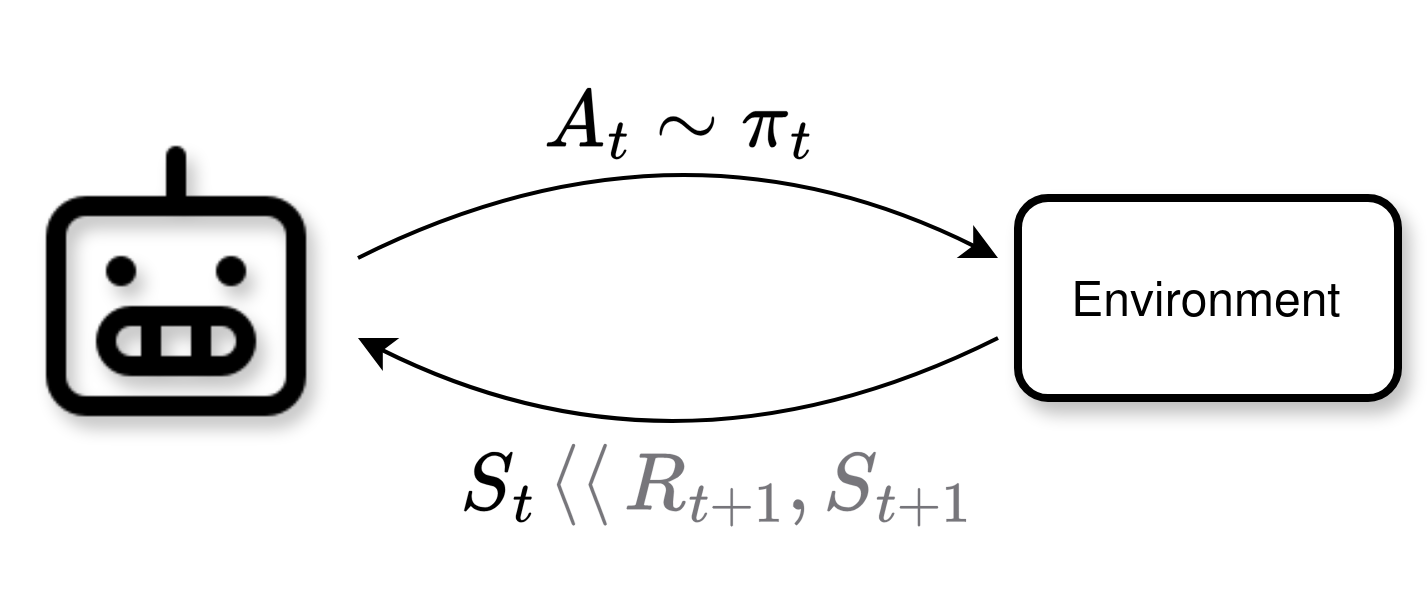
\includegraphics[width=0.65\textwidth]{figures/RL_loop.png}
%     \caption{Caption}
%     \label{fig:rl_loop}
% \end{figure}

\subsection{Policies}
% Policies specify decision rules within the context of RL and determines which action the agent should use next. Policies are divided in several categories,
% \begin{itemize}
%     \item Stationary, if the policy $\pi$ remain the same for any time $t$, or non-stationary, when the policy $\pi_t$ depends on the time $t$.
%     \item Deterministic, if the policy $\pi:\cS\rightarrow\cA$ determines a single action, or randomized, if instead the policy $\pi:\cS\rightarrow\Delta(\cA)$ is a distributions over actions.
%     \item A polciy can be defined over the set of histories $\pi:\cH\rightarrow\cA$ or can be Makovian, if $\pi:\cS\rightarrow\cA$ depends solely on the current state.
% \end{itemize}
% On what follows, we will assume policies to be stationary, Markovian and randomized unless otherwise specified.

\subsection{Optimality criteria}

% RL algorithms try to find an optimal policy that maximizes some sort of numerical objective. Throughout this work, the following optimality criteria will be used~\citep{Puterman1994},

% \begin{itemize}
%     \item In the \textbf{average reward} setting, an optimal policy is one that maximizes the reward rate per step, also called or gain or just optimal average reward, defined as,
%     \begin{equation}
%         \rho^\pi = \lim_{N\rightarrow\infty}{\frac 1 N}\EEc{\sum_{i=t}^N\cR(S_{i}, A_i, S_{i+1})}{S_t=s, A_i\sim\pi(S_t), S_{t+1}}
%     \end{equation}
%     \item For the \textbf{discounted} case, the definition of an MDP 
%      \begin{equation}
%         \EEc{\sum_{i=t}^\infty \gamma^{i-t} \cR(S_{i}, A_i, S_{i+1})}{\pi}
%     \end{equation}
%     \item \textbf{Total reward}: 
%     \begin{equation}
%         \EEc{\sum_{i=t}^T \cR(S_{i}, A_i, S_{i+1})}{\pi}
%     \end{equation}
% \end{itemize}


\subsection{Value functions}

\subsection{Dynamic programming}

\subsection{Function approximation}


\guillermo{
\section{Successor features} DEVELOP THIS FURTHER .. 

\label{section:successor_features}

Successor features (SFs)~\citep{Dayan1993, Barreto2017} is a widely used RL representation framework that assumes the reward function is linearly expressible with respect to a feature vector,
\begin{equation}
  \cR^\w(s, a, s') = \w^\intercal\boldsymbol\phi(s, a , s').
  \label{eq:reward_sf}
\end{equation}

Here, $\boldsymbol\phi:\cS\times\cA\times\cS\rightarrow\real^{d}$ maps transitions to feature vectors and $\w\in\real^d$ is a weight vector. Every weight vector~$\w$ induces a different reward function and, thus, a task. The SF vector of a state-action pair $(s,a)\in\cS\times\cA$ under a policy $\pi$ is the expected discounted sum of future feature vectors: 
\begin{equation}
  \boldpsi^\pi(s, a) = \EEcp{\sum_{i=t}^\infty \gamma^{i-t} \boldsymbol\phi_i}{S_t = s, A_t = a}{\pi},
  \label{eq:sf}
\end{equation}
where $\boldsymbol\phi_i = \boldsymbol\phi(S_{i}, A_{i}, S_{i+1})$. The action value function for a state-action pair $(s, a)$ under policy $\pi$ can be efficiently represented using the SF vector. Due to the linearity of the reward function, the weight vector can be decoupled from the Bellman recursion. Following the definition of Equations~\eqref{eq:qfunction}~ and \eqref{eq:reward_sf}, the action value function in the SF framework can be rewritten as
\begin{align}
  Q^\pi_\w(s, a) &= \EEcp{\sum_{i=t} ^\infty \gamma^{i-t} \w^\intercal\boldsymbol\phi_i}{S_t = s, A_t = a}{\pi} \nonumber \\
                 & = \w^\intercal\EEcp{\sum_{i=t} ^\infty \gamma^{i-t} \boldsymbol\phi_i}{S_t = s, A_t = a}{\pi} \nonumber \\
                 &=  \w^\intercal \boldpsi^\pi(s, a) .
\label{eq:qfunction_sf}
\end{align}

The SF representation leads to \textit{generalized policy evaluation} (GPE) over multiple tasks~\citep{Barreto2020a}, and similarly, to \textit{generalized policy improvement} (GPI) to obtain new better policies~\citep{Barreto2017}.

A family of MDPs is defined as the set of MDPs that share all the components, except the reward function. This set is formally defined as 
\begin{equation*}
    \cM^{\boldsymbol{\phi}}\equiv\{\langle\cS,\cE,\cA,\cR_\w,\mathbb{P}_0, \mathbb{P},\gamma\rangle \lvert \cR_\w = \w^\intercal \boldsymbol{\phi}, \forall\w\in\real^d\}.
\end{equation*}

Transfer learning on families of MDPs is possible thanks to GPI. Given a set of policies $\Pi$, learned on the same family~$\cM^{\boldsymbol{\phi}}$, for which their respective SF representations have been computed, and a new task $\w'\in\real^d$, a GPI policy $\pi_{\text{GPI}}$ for any $s\in\cS$ is derived as 
\begin{equation}
    \pi_{\text{GPI}}(s) \in \argmax_{a\in\cA} \max_{\pi\in\Pi} Q^\pi_{\w'}(s, a).
    \label{eq:gpi}
\end{equation}

However, there is no guarantee of optimality for $\w'$.
A fundamental question to solve the so-called \textit{optimal policy transfer learning problem} is which policies should be included in the set of policies $\Pi$ so an optimal policy for any weight vector $\w\in\real^d$ can be obtained with GPI. 
}

\section{Linearly-solvable Markov decision processes}

Linearly-solvable Markov decision processes are a restricted class of the more general MDPs where the Bellman optimality equations are linear. This makes the computation of optimal value functions more efficient. In continuous state space domains or contexts of optimal control as probablistic inference, they frequently appear under the names of path-integral or Kullback-Leibler control~\citep{Kappen2012}. 

However, this formulation is arguably restricted and only applicable to domains with deterministic dynamics. Nonetheless, the intuition of entropy-regularization~\citep{Neu2017}, that lies at the core of LMDPs, is fundamental in RL as it is one of the building blocks of current state-of-the-art deep reinforcement learning algorithms such as or Trust Region Policy Optimization~\citep{Schulman2015}, soft actor-critic (SAC)~\citep{Haarnoja2018} or Manchausen RL~\citep{Vieillard2020}.

\subsection{First-exit linearly-solvable Markov decision processes}

A first-exit linearly-solvable Markov decision process, or just LMDP~\citep{Todorov2006,Kappen2005}, is defined as a tuple $\cL=\langle\cS,\cT,\kernel,\cR,\cJ\rangle$, where: \begin{itemize}
  \item $\cS$ is a set of non-terminal states.
  \item $\cT$ is a set of terminal states.
  \item $\kernel:\cS\rightarrow\Delta(\cS^+)$ is an uncontrolled transition function, also known as passive dynamics or passive controls.
  \item $\cR:\cS\rightarrow\real$ is a reward function for non-terminal states.
  \item $\cJ:\cT\rightarrow\real$ is a reward function for terminal states.
\end{itemize}

\noindent Let $\cS^+=\cS\cup\cT$ denote the full set of states and $B=\max_{s\in\cS}|\cB(\kernel(\cdot|s))|$ an upper bound on the support of $\kernel$. 

Similarly to the stardard RL learning loop, the agent interacts with the environment in a sequential manner. Nontheless, since there are no explict actions, the learning agent now follows a policy $\pi:\cS\rightarrow\Delta(\cS^+)$. Such a policy chooses, for each non-terminal state $s\in\cS$, a probability distribution over next states in the support of $\kernel(\cdot|s)$, i.e.~$\pi(\cdot|s)\in\Delta(\cB(\kernel(\cdot|s))$. There is also no explicit mention to the initial state distribution, which is asummed to be uniform over the set of non-terminal states (~i.e. $\kernel_0 = \text{unif}(\cS)$). 

At each timestep $t$, the learning agent observes a state $s_t\in\cS^+$. If $s_t$ is non-terminal, the agent transitions to a new state $s_{t+1}\sim\pi(\cdot|s_t)$ and receives an immediate, regularized reward
\[
\cR(s_t, s_{t+1},\pi) = \cR(s_t) - \frac 1 \eta \log \frac {\pi(s_{t+1}|s_t)} {\kernel(s_{t+1}|s_t)},
\] 
where $\cR(s_t)$ is the reward associated with state $s_t$, and $\eta$ is a temperature parameter. 
%  $\mathrm{KL}(\pi(\cdot|s_t)\Vert\, \kernel(\cdot|s_t))$ is the Kullback-Leibler divergence between $\pi(\cdot|s_t)$ and $\kernel(\cdot|s_t)$ defined as 
% \begin{equation*}
%   \mathrm{KL}(\pi(\cdot|s)\Vert\, \kernel(\cdot|s)) = \sum_{s'} \pi(s'\lvert s) \log \frac{\pi(s'\lvert s)}{\kernel(s'\lvert s)}
% \end{equation*}

Hence the agent can set the probability $\pi(s_{t+1}|s_t)$ freely, but gets penalized by the entropy-regularization term for deviating from the passive controls $\kernel(s_{t+1}|s_t)$, and this penalty is modulated by the temperature parameter $\eta$. On the other hand, if $s_t$ is terminal, the agent receives reward $\cJ(s_t)$ and then the current episode ends. The aim of the agent is to compute a policy $\pi$ that maximizes the expected future \textbf{total reward}. Thus, for each non-terminal state $s\in\cS$, the value function is defined as
\[
v^\pi_\eta(s) = \EEc{\sum_{i=t}^{T-1} \cR(S_i, S_{i+1},\pi) + \cJ(S_T)}{S_t = s, \pi}.
\]

Here, $T$ is a random variable representing the time at which the current episode ends, and $S_t$ is a random variable representing the state at time $t$. The expectation is over the stochastic choice of next state $S_{t+1}\sim\pi(\cdot|S_t)$ at each time~$t$, and the time $T$ it takes for the episode to end. It is assumed that the reward of all non-terminal states is negative, i.e.~$\cR(s)<0$ for each $s\in\cS$. As a consequence, $\cR(s,\pi)<0$ holds for any policy $\pi$, and the value $v^\pi_\eta(s)$ has a well-defined upper bound. Note that the value function is computed with respect to a concrete value of the temperature parameter $\eta$.  
%As an alternative to the assumption $\cR(s)<0$, we could instead assume that each policy terminates with probability 1 within a fixed time horizon $H$.


Finding the optimal policy implies computing the optimal value function ${v^*_\eta:\cS\rightarrow\real}$, i.e.~the maximum expected future total reward among all policies. The value function is extended to each terminal state $\tau\in\cT$ by defining $v^*_\eta(\tau)\equiv\eta\cJ(\tau)$. The value function $v^*_\eta$ satisfies the Bellman equations
\begin{align*}
  \eta v^*_\eta(s) &= \eta \max_\pi \left[ \cR(s,\pi) + \mathbb{E}_{s'\sim\pi(\cdot|s)} v^*_\eta(s') \right] \\
  &= \eta \cR(s) + \max_\pi \mathbb{E}_{s'\sim\pi(\cdot|s)} \left[ \eta v^*_\eta(s') - \log \frac {\pi(s'|s)} {\kernel(s'|s)} \right] \;\; \forall s.
\end{align*}
In expectation, the regularization term in reduces to the Kullback-Liebler divergence between $\pi$ and $\kernel$,
\begin{equation*}
  \mathbb{E}_{s'\sim\pi(\cdot|s)} \log \frac {\pi(s'|s)} {\kernel(s'|s)} = \sum_{s'}\kernel(s'\lvert s)\log\frac{\pi(s'\lvert s)}{\kernel(s'\lvert s)} = \mathrm{KL}\big(\pi(\cdot|s)\Vert\, \kernel(\cdot|s)\big).
\end{equation*}

The maximization in the Bellman equations can be resolved analytically~\citep{Todorov2006}, and the expression above can be rewritten as
\begin{align*}
  v^*_\eta(s)      &=  \frac 1 \eta \log{\sum_{s'\in\cS}\kernel(s'\lvert s)e^{\eta(\cR(s) + v^*_\eta(s'))})} \;\;\forall s\in\cS, \\
                   &=  \cR(s) + \frac 1 \eta \log{\sum_{s'\in\cS}\kernel(s'\lvert s)e^{\eta v^*_\eta(s')}} \;\;\forall s\in\cS, \\
  \eta v^*_\eta(s) &=  \eta \cR(s) + \log{\sum_{s'\in\cS}\kernel(s'\lvert s)e^{\eta v^*_\eta(s')}} \;\;\forall s\in\cS.
\end{align*}
Now, consider the notation $z(s)=e^{\eta v^*_\eta(s)}$ for each $s\in\cS^+$. This notation is often abused by referring to $z(s)$ as the (optimal) value of $s$. After exponentiating, the previous system yields the following Bellman optimality equations that are linear in $z$:
\begin{equation}\label{eq:boe_z_lmdp}
z(s) = e^{\eta\cR(s)} \sum_{s'}\kernel(s'|s)z(s').
\end{equation}
\subsubsection{Solving a first-exit LMDP}
The Bellman equation can be expressed in matrix form by defining an $\lvert\cS\rvert\times\lvert\cS\rvert$ diagonal reward matrix $R=\diag(e^{\eta\cR(\cdot)})$ and an $\lvert\cS\rvert\times \lvert\cS^+\rvert$ stochastic transition matrix $P$ whose entries $(s,s')$ equal $\kernel(s'|s)$. Define a vector $\bf z$ that stores the values $z(s)$ for each non-terminal state $s\in\cS$, and a vector $\bf z^+$ extended to all states in $\cS^+$. Now the Bellman equations are written in matrix form:
\begin{equation}\label{eq:eigen_lmdp}
{\bf z} = R P {\bf z^+}.
\end{equation}
Given $z$, the optimal policy $\pi$ is given by the following expression for each pair of states $(s,s')$:
\begin{equation}
\label{eq:lmdp_optimal_policy}
\pi(s'|s) =  \frac {\kernel(s'|s) e^{\eta v(s')} } {\sum_{s''} \kernel(s''|s) e^{\eta v(s'')} } = \frac {\kernel(s'|s)z(s')} {\sum_{s''} \kernel(s''|s)z(s'')}.
\end{equation}

The solution for $z$ corresponds to the largest eigenvector of $RP$.
If the dynamics $\kernel$ and $\cR$ are known, one can iterate~\eqref{eq:eigen_lmdp}~\citep{Todorov2006}.

Alternatively, an estimate $\widehat{z}$ can be learned incrementally using stochastic updates based on state transitions sampled from the uncontrolled dynamics $(s_t,r_t,s_{t+1})$
% use an online algorithm called Z-learning to compute an estimate  \citep{TodorovNIPS2007}. After observing each transition , the update rule of Z-learning is given by
\[
\widehat{z}(s_t) \leftarrow (1-\alpha_t)\widehat{z}(s_t) + \alpha_t e^{\eta r_t}\widehat{z}(s_{t+1}),
\]
where $\alpha_t$ is a learning rate. 
The above update rule is called \emph{Z-learning}~\citep{Todorov2006} and suffers from slow convergence in very large state spaces and when the optimal policy differs substantially from the uncontrolled dynamics $\kernel$.
%assumes that we sample next states using the uncontrolled transition function $\cP$, which is typically no better than a random walk. 
A better choice is importance sampling, which uses samples from the estimated policy $\widehat{\pi}$ derived from the estimated values $\widehat{z}$ and \eqref{eq:lmdp_optimal_policy} and updates $\widehat{z}$ according to the following update
%to obtain samples that are corrected using the following update~\citet{TodorovPNAS2009}:
%to sample In this case,  suggested a corrected update rule based on importance sampling:
\begin{align}\label{eqn:zlearning-imp}
\widehat{z}(s_t) \leftarrow (1-\alpha_t)& \widehat{z}(s_t) + \alpha_t e^{\eta r_t}\widehat{z}(s_{t+1})\frac {\kernel(s_{t+1}|s_t)} {\widehat{\pi}(s_{t+1}|s_t)}.
\end{align}
However, this requires local knowledge of $\kernel(\cdot|s_t)$ to correct for the different sampling distribution.
%, i.e.~the set of possible next states and their associated uncontrolled probabilities.
Though this seems like a strong assumption, in practice $\kernel$ usually has a simple form, e.g.~uniform distribution.
Further, as shown in \citep{Jonsson2016}, the corrected update rule in \eqref{eqn:zlearning-imp} can also be used to perform off-policy updates in case transitions are sampled using a policy different from $\widehat{\pi}$.
%leading to simultaneous learning of different tasks.
%Note that the expression for the policy $\widehat{\pi}$ in \eqref{eq:pi} and the corrected update rule in \eqref{eqn:zlearning-imp} require local knowledge of $\cP(\cdot|s_t)$, i.e.~the set of possible next states and their associated uncontrolled probabilities. Though this seems like a strong assumption, in practice $\cP$ usually has a simple form, e.g.~uniform. \citet{conf/icaps/Jonsson16} showed that the corrected update rule in \eqref{eqn:zlearning-imp} can also be used to perform off-policy updates in case transitions are sampled using a policy different from $\widehat{\pi}$.

\subsubsection{Compositionality}
\label{section:compositionality}
\citet{Todorov2009a} introduces the concept of compositionality for LMDPs. Consider a set of LMDPs $\{\cL_1,\ldots,\cL_n\}$, where each LMDP $\cL_i=\langle\cS,\cT,\kernel,\cR,\cJ_i\rangle$ has the same components $\cS,\cT,\kernel,\cR$ and only differ in the reward $\cJ_i(\tau)$ of each terminal state $\tau\in\cT$, as well as its exponentiated value $z_i(\tau)=e^{\eta \cJ_i(\tau)}$.

Now consider a new LMDP $\cL=\langle\cS,\cT,\kernel,\cR,\cJ\rangle$ with the same components as the $n$ LMDPs above, except for $\cJ$. Assume that there exist weights $w_1,\ldots,w_n$ such that the exponentiated value of each terminal state $\tau\in\cT$ can be written as
\[
e^{\eta \cJ(\tau)} = z(\tau) = w_1z_1(\tau) + \ldots + w_nz_n(\tau) = \sum_{k=1}^n w_kz_k(\tau).
\]
Since the Bellman optimality equation of each non-terminal state $s\in\cS$ is linear in $z$, the optimal value of $s$ satisfies the same equation:
\[
z(s) = \sum_{k=1}^n w_kz_k(s).
\]
Consequently, if previously compute the optimal values $z_1,\ldots,z_n$ of the $n$ LMDPs are previously computed and the weights $w_1,\ldots,w_n$ are known, one immediately obtains the optimal values of the new LMDP $\cL$ without learning.


\subsection{Average-reward linearly-solvable Markov decision processes}

LMDPs can be extended to the average-reward setting. An average-reward Linearly-solvable Markov decision process (ALMDP) is a tuple
$\cL = \langle\cS,\kernel,\cR\rangle$, where $\cS$ is a set of states, $\kernel:\cS\rightarrow\Delta(\cS)$ is the passive dynamics, and $\cR$ is the reward function. Unlike first-exit LMDPs, there are no terminal states, since ALMDPs represent infinite-horizon (continuing) tasks and, therefore, there is no reward function for terminal states.  

The following assumptions are made about ALMDPs. These are common assumptions in the average-reward RL setting to avoid ill-defined value functions.

\begin{assumption}
  The ALMDP $\cL$ is communicating~\citep{Puterman1994}: for each pair of states $s,s'\in\cS$, there exists a policy $\pi$ that has non-zero probability of reaching $s'$ from $s$.
  \label{ass:communicating}
\end{assumption}

\begin{assumption}
  The ALMDP $\cL$ is unichain~\citep{Puterman1994}: the transition probability distribution induced by all stationary policies admit a single recurrent class.
  \label{ass:unichain}
\end{assumption}
%\todo{I think this assumption is enough: no need to introduce the notation for stationary distributions over the state space since we do not use it at any point. This assumption as is is enough to make the gain not to be conditioned by the initial state.}
%{\color{red} \begin{assumption}
%  For all states $s\in\cS$ the reward $\cR(s)$ is bounded in $\left(-\infty, 0\right]$.
%  \label{ass:rewards}
%\end{assumption}}

In the average-reward setting, the value function is defined as the expected \textbf{average reward} when following a policy $\pi:\cS\rightarrow\Delta(\cS)$ starting from a state $s\in\cS$. This is expressed as
\begin{equation}
  v_\eta^\pi(s) = \underset{T\rightarrow\infty}\lim \EEc{\frac{1}{T} \sum_{i=t}^T \cR(S_i, S_{i+1}, \pi)}{S_t = s, \pi},
  \label{eq:value_function_almdp}
\end{equation}
where $\cR(s_t, s_{t+1}, \pi)$ is defined as for first-exit LMDPs.
Again, the goal is to obtain the optimal value function $v^*_\eta$. Under Assumption~\ref{ass:unichain}, the Bellman optimality equations can be written as
\begin{equation}
  v^*_\eta(s) = \frac 1 \eta \log{\sum_{s'\in\cS}\kernel(s'\lvert s)e^{\eta(\cR(s) - \rho + v^*_\eta(s'))}} \;\;\forall s\in\cS,
  \label{eq:boe_almdp}
\end{equation}
where $\rho$ is the optimal one-step average reward (i.e.~gain), which is state-independent for unichain\todo{Add derivation of the independece of the gain?} ALMDPs~\citep{Todorov2006}. Exponentiating yields
\begin{equation}
  z(s) = e^{\eta(\cR(s) - \rho)} \sum_{s'\in\cS}\kernel(s'\lvert s)z(s') \;\;\forall s\in\cS.
  \label{eq:boe_z_almdp}
\end{equation}
For the optimal value function $z$, the optimal policy is given by the same expression as in~\eqref{eq:lmdp_optimal_policy}.

\subsubsection{Solving an ALMDP}

Let $\Gamma=e^{\eta\rho}$ denote the exponentiated gain. Similar to the first-exit case, Equation~\eqref{eq:boe_z_almdp} can be expressed in matrix form as
\begin{equation}\label{eq:rel_opt}
  \Gamma {\bf z} = R P {\bf z},
\end{equation}
where the matrices $P\in \real^{\lvert\cS\rvert\times\lvert\cS\rvert}$ and $R\in \real^{\lvert\cS\rvert\times\lvert\cS\rvert}$ are appropiately defined as in~\eqref{eq:eigen_lmdp}. The exponentiated gain $\Gamma$ can be shown to correspond to the largest eigenvalue of $RP$~\citep{Todorov2009}.
An ALMDP can be solved using {\em relative value iteration} by selecting a reference state $s^*\in\cS$, initializing $\widehat{\bf z}_0={\bf 1}$ and iteratively applying
\begin{equation*}
  \widehat{\bf z}_{k+\frac 1 2} \gets R P \widehat{\bf z}_k, \quad \quad \widehat{\bf z}_{k+1} \gets \widehat{\bf z}_{k+\frac 1 2} / \widehat z_{k+\frac 1 2}(s^*).
\end{equation*}
The reference state $s^*$ satisfies $z(s^*)=1$, which makes the optimal value $z$ unique (else any constant shift preserves optimality). After convergence, the exponentiated gain equals $\Gamma=\widehat z_{k+\frac 1 2}(s^*)$. Under Assumption~\ref{ass:communicating}, relative value iteration converges to the unique optimal value $z$~\citep{Todorov2009}.

Analogously to first-exit LMDPs, when $\kernel$ and $\cR$ are not known, the agent can learn estimates $\widehat z$ and $\widehat\Gamma$ of the optimal value function and the exponentiated gain in an online manner, using samples $(s_t, r_t, s_{t+1})$ generated when following the estimated policy $\widehat\pi$. The update rules for the so-called differential Z-learning algorithm are given by
\begin{align}
  \widehat{z}_{t+1}(s_t)  \gets \widehat{z}_{t}(s_{t}) & + \alpha_t \Bigg(\frac{e^{\eta r_t}}{\widehat\Gamma_t}\dfrac{\kernel(s_{t+1}\lvert s_t)}{\widehat\pi_t(s_{t+1}\lvert s_t)}  - \widehat z_t(s_t)\Bigg),\label{eq:diff_update_z}  \\   %\delta^z_t \\
  \widehat\Gamma_{t+1}    \gets \widehat\Gamma_t       & + \beta_t \Bigg(\frac{e^{\eta r_t}}{\widehat z_t(s_t)}\dfrac{\kernel(s_{t+1}\lvert s_t)}{\widehat\pi_t(s_{t+1}\lvert s_t)}  - \widehat \Gamma_t\Bigg).\label{eq:diff_update_gamma}
\end{align}
The learning rates $\alpha_t$ and $\beta_t$ can be chosen independently.

Unlike the first-exit case, the compositionality property does not hold in the average-reward case.

\subsection{Function approximation in LMDPs}

So far, all the results introduced for (A)LMDPs restrict to the tabular case where the full state space can be enumerated and stored in memory. However, in cases where the state space is considerably large, tabular methods are unfeasible and the value function is approximated.

In this line,~\cite{Todorov2010} prescibes two families of methods for adapting LMDPs in the average-reward setting for function approximation. The first one lies in the family of policy gradients while the second ones can be considered critic-only approaches. Here a valid parameterization of the policy $\pi(s'\lvert s, \w)$ is considered.

The Bellman equation~\eqref{eq:boe_almdp} can be rewritten as follows
\begin{equation}
\label{eq:boe_for_pg}
\rho + v^*(s) =\cR(s) +\log{\sum_{s'\in\cS}\kernel(s'\lvert s)e^{v^*(s')}} \;\;\forall s\in\cS,
\end{equation}
for the sake of simplicity it is assumed that $\eta=1$. 

The first flavor of methods builds on the policy gradient theorem for ALMDPs~\citep[cf.~Theorem 1]{Todorov2010} that states that the gradient of the gain in ALMDPs is
\begin{equation}
  \nabla_\w \rho = \sum_{s}\mu(s, \w) \sum_{s'} \nabla_\w \pi(s'\lvert s, \w)\Big( \log \frac{\pi(s'\lvert s, \w)}{\kernel(s'\lvert s)} + \widetilde v(s', \mathbf{r})\Big),
\end{equation}
where $\mu(x, \w)$ is the stationary distribution induced by $\pi$ and $\widetilde v(s,\mathbf{r})$ an approximation to the (optimal) value function with parameterization $\mathbf r$.

For the second type of methods one could use \textit{approximate} value iteration or \textit{approximate} policy iteration to iteratively improve the weight vector $\w$, even though this results in a bias estimator. An even more direct approach is to use Gauss-Newton method to fit the weight vector $\w$ by directly optimizing~\eqref{eq:boe_for_pg}.

Despite the correctness of the theoretical results, which guarantee that function approximation can be used along with LMDPs, they are of little practical use. Even in the linear function approximation (LFA) case, obtaining a correct parameterization for $\widetilde v(s,\mathbf{r})$ requires of an intricate process in the policy gradient approach. Additionally, the representation of the policy still depends on the size of the whole state space. This makes the approach intractable for real-world problems as it dos not scale for extremely large state spaces.


\section{Hierarchical Reinforcement Learning}
Hierarchical Reinforcement learning embodies the idea of divide-and-conquer in sequential decision problems. 
\subsection{Optimality of HRL algorithms}
\cite{Dietterich2000} identifies two types of optimality for hierarchical methods in reinforcement learning, namely \textit{hierarchical optimality} and \textit{recursive optimality}. Hierarchical optimality implies optimality with regard a constrained space of policies, given by the hierarchy structure. Hierarchies of Abtract Machines (HAMs,~\cite{Parr1997}) and the Options Framework~\citep{Sutton1999} lie in this category) 
\subsection{The options framework}
\label{section:options}

\section{Non-Markovian task specification}
\label{section:non_markovian}
 {\color{blue}
 
 \begin{itemize}
 \item Difficulty about expressing some tasks in Marokovian terms 
 \item Finite State Autamatons and Reward Machines 
 \item Reward Machines and their relationship with logics
 \item Comment on algorithms given in the 
  
\end{itemize}
 
 }




\chapter{Globally Optimal Hierarchical Reinforcement Learning for Linearly-solvable Markov Decision Processes}
\section{Introduction}
A major challenge in reinforcement learning is to design agents that are able to learn efficiently and to adapt their existing knowledge to solve new tasks. As it has been discussed, one way to reduce the complexity of learning is hierarchical reinforcement learning~\citep{Sutton1999, Dietterich2000, Barto2003}. In this Chapter, we propose a novel approach to hierarchical reinforcement learning in LMDPs that takes advantage of the compositionality of LMDPs. This approach assumes that the state space is partitioned into subsets, and the subtasks consist in moving between these partitions. The subtasks are parameterized on the current value estimates of boundary states. 

In section~\ref{section:compositionality}, compostionality was shown to be one of the computational advantages of LMDPs, which allows for zero-shot learning of new skills by linearly combining previously learned base skills which only differ in their cost or reward at boundary states~\citep{Todorov2009,Silva2009}.  In this work, instead of solving the subtasks each time the value estimates change, the compositionality property of LMDPs is exploited to express the solution to an arbitrary subtask as a linear combination of a set of base LMDPs. The result is a form of value function decomposition which allows expressing an estimate of the optimal value of an arbitrary state as a combination of multiple value functions with smaller domains.

In this chapter, we present two novel algorithms. The first is a two-step eigenvector when both the passive dynamics and the reward functions are known. When these are unknown to the learning agent, an online algorithm can be used to simultaneously learn the value function of the subtasks and the value for the boundary states. 
We accompany the theoretical results with a empirical evaluation of the learning agent on two classic control problems.

\section{Contributions}
\begin{itemize}
%\item We define a novel scheme based on compositionality for solving subtasks, defining local reward functions that constitute a convenient basis for composite reward functions.
\item To define a novel scheme based on compositionality for solving subtasks, defining local rewards that constitute a convenient basis for composite rewards.
\item The subtask decomposition is at the level of the value function, not of the actual policy. Hence the proposed approach does not suffer from non-stationarity in the online setting, unlike approaches that select among subtasks whose associated policies are being learned.
\item Even though the subtasks have local reward functions, under mild assumptions the proposed approach converges to the globally optimal value function.
\item The proposed learning algorithm is analyzed empirically and it shows in two classical domains 
that it is more sample efficient compared to a flat learner and similar hierarchical approaches when the set of boundary states is smaller than the entire state space.
\end{itemize}


\section{Related Work}
Several authors have recently exploited concurrent compositionality of tasks in the context of transfer learning.~\citet{Niekerk2019} use the linear compositionality of LMDPs to solve new tasks that can be expressed as combinations of a series of existing base tasks. They show that, while disjunctions of base tasks (OR-compositionality) can be performed exactly, the AND composition (when the goals of base tasks partially overlap) can only be performed approximately.

\citep{Haarnoja2018a} exploit a similar idea to transfer knowledge from existing tasks to new tasks by averaging their reward functions.~\citep{Hunt2019} further extended this by introducing the so-called compositional optimism, and apply divergence correction in case compositionality does not transfer well.

More recently, \citep{NangueTasse2020} derive a formal characterization of union and intersection of tasks in terms of Boolean algebra. They show that learning (extended) value functions that account for all achievable goals, exact zero-shot transfer learning using both AND- and OR- compositionality is possible, achieving an exponential increase in skills compared to the previous works.

All the aforementioned results are derived for general MDPs with deterministic dynamics and, possibly, entropy regularization. This setting is no more general than the class of LMDPs.

%~\textit{van2019composing} use compositionality in systems with deterministic dynamics to solve new tasks that can be expressed as combinations of a series of existing tasks. The authors distinguish between AND-compositionality and OR-compositionality, depending on whether the features of a new task are present in all existing tasks or only some.
%and present a method that approximates AND-compositionality and 

%The above forms of compositionality do not guarantee that the resulting policy is optimal, unlike compositionality for LMDPs which is exact.
The aim of this work is to integrate both concurrent task composition, as done in the above approaches, together with hierarchical composition, where skills are chained in a temporal sequence, under the framework of LMDPs.

Several authors have proposed hierarchical versions of LMDPs.~\cite{Jonsson2016} extend MAXQ~\citep{Dietterich2000} to LMDPs by defining subtasks that represent high-level decisions. The top-level policy chooses multi-step transitions, which introduces non-stationarity in the high-level decision process if subtasks are learned concurrently, and also prevents global optimality. The authors discuss the idea of compositionality, but do not explore the concept further.
~\citet{Saxe2017} propose a hierarchical multi-task architecture that does exploit compositionality. Their multitask LMDP maintains a parallel distributed representation of tasks, reducing the complexity through stacking. However, the approach requires to augment the state space with many additional boundary (subtask) states. Further, the stacking introduces additional costs (cf. their Equation 10), and does not provide global optimality.

The options keyboard \citep{Barreto2019} combines a successor feature representation with generalized policy improvement to obtain subtask policies from a set of base subtasks without learning, similar to subtask compositionality used in the proposed method. However, unlike in this, their composition weights have to be set manually, and although the composed policy is guaranteed to be better than the individual base policies, it is not guaranteed to be optimal.

%\textit{multipl}

The proposed method is similar to that of \citet{Wen2020} since a hierarchical decomposition based on a partition of the state space is defined, and exploit the equivalence of subtasks to reduce the learning effort. Unlike previous work, however, our approach is not restricted to single initial states, does not suffer from non-stationarity in the online setting, proposes a more general definition of equivalence that captures more structure, and guarantees convergence to the optimal value function for stochastic dynamics.

The concept of equivalent subtasks is strongly related to factored (L)MDPs, which capture conditional independence among a set of state variables~\citep{Boutilier1995, Koller2000}. Equivalence arises whenever a subset of state variables are conditionally independent of another subset. Several authors have shown how to automatically discover the structure of factored MDPs from experience~\citep{Strehl2007,Kolobov2012}, which in turn could be used to define equivalence classes of subtasks.

%{\color{red} Mention here the other papers \textit{hunt2019composing}\textit{van2019composing},\textit{algebra}}

\section{Hierarchical LMDPs}

In this section we describe our novel approach to hierarchical LMDPs. We first describe the particular form of hierarchical decomposition that we consider, and then present algorithms for solving a decomposed LMDP.

\subsection{Hierarchical Decomposition}

Our hierarchical decomposition is similar to that of~\citep{Wen2020}. Formally, given an LMDP $\cL=\langle\cS,\cT,\kernel,\cR,\cJ\rangle$, the set of non-terminal states $\cS$ is partitioned into $L$ subsets $\{\cS_i\}_{i=1}^L$. For each such subset $\cS_i$, there exists an induced subtask $\linebreak {\cL_i=\langle\cS_i,\cT_i,\kernel_i,\cR_i,\cJ_i\rangle}$, i.e.~an LMDP whose components are defined as follows:
\begin{itemize}
\item The set of non-terminal states is $\cS_i$.
\item The set of terminal states $\cT_i=\{\tSi \in\cS^+\setminus\cS_i:\exists s\in \cS_i \; \text{s.t.} \; \tSi \in \cB(\kernel(\cdot|s))\}$ includes all states in $\cS^+\setminus\cS_i$ (terminal or non-terminal) that are reachable in one step from a state in $\cS_i$.
\item $\kernel_i:\cS_i\rightarrow\Delta(\cS_i^+)$ and $\cR_i:\cS_i\rightarrow\real$ are the restrictions of $\kernel$ and $\cR$ to $\cS_i$, where $\cS_i^+=\cS_i\cup\cT_i$ denotes the full set of subtask states.
%\item The reward of a terminal state $\tS\in\cT_i$ equals $\cJ_i(\tS)=\cJ(\tS)$ if $\tS\in\cT$, and $\cJ_i(\tS)=\widehat{v}(\tS)$ otherwise, where $\widehat{v}(\tS)$ is the estimated value in $\cL$ of the non-terminal state in  $\tS\in\cS \setminus \cS_i$.
\item The reward of a terminal state $\tSi \in\cT_i$ equals $\cJ_i(\tSi)=\cJ(\tSi)$ if $\tSi\in\cT$, and $\cJ_i(\tSi)=\widehat{v}(\tSi)$ otherwise, where $\widehat{v}(\tSi)$ is the estimated value in $\cL$ of the non-terminal state in  $\tSi\in\cS \setminus \cS_i$.
\end{itemize}

Intuitively, if the reward $\cJ_i(\tSi)$ of each terminal state $\tSi\in\cT_i$ equals its optimal value $v(\tSi)$ for the original LMDP~$\cL$, then solving the subtask $\cL_i$ yields the optimal values of the states in $\cS_i$.
In practice, however, we use an estimate $\widehat{v}(\tSi)$ of the optimal value.

In this case, the subtask $\cL_i$ is {\em parameterized} on the value estimate $\widehat{v}$ of terminal states in $\cT_i$, and each time the value estimate changes, $\cL_i$ can be solved to obtain a new value estimate
$\widehat{v}(s)$ for each state $s\in\cS_i$.



Let $\cE=\cup_{i=1}^L\cT_i$ be a set of {\em exit states}, i.e.~the union of the terminal states of each subtask in $\{\cL_1,\ldots,\cL_L\}$. For convenience, let $\cE_i=\cE\cap\cS_i$ denote the set of (non-terminal) exit states in the subtask $\cL_i$. Also, consider the notation $K=\max_{i=1}^L|\cS_i|$, $N=\max_{i=1}^L|\cT_i|$ and $E=|\cE|$.

The notion of subtasks is just like in~\citep{Wen2020}.
\begin{definition}
Two subtasks $\cL_i$ and $\cL_j$ are equivalent if there exists a bijection $f:\cS_i\rightarrow\cS_j$ such that the transition probabilities and rewards of non-terminal states are equivalent through $f$.
\end{definition}
Unlike \citep{Wen2020}, this definition does {\em not} require the sets of terminal states $\cT_i$ and $\cT_j$ to be equivalent. Instead, for each class of equivalent subtasks, the approach is to define a single subtask whose set of terminal states is the {\em union} of the sets of terminal states of subtasks in the class.

Formally, a set of equivalence classes $\cC=\{\cC_1,\ldots,\cC_C\}$ is defined, $C\leq L$, i.e.~a partition of the set of subtasks $\{\cL_1,\ldots,\cL_L\}$ such that all subtasks in a given partition are equivalent. Only a single subtask $\cL_j=\langle\cS_j,\cT_j,\kernel_j,\cR_j,\cJ_j\rangle$ needs to be represented per equivalence class $\cC_j\in\cC$. The components $\cS_j,\kernel_j,\cR_j$ are shared by all subtasks in the equivalence class, while the set of terminal states is $\cT_j=\bigcup_{\cL_i\in\cC_j} \cT_i$, where the union is taken w.r.t. the bijection $f$ relating all equivalent subtasks. As before, the reward $\cJ_j$ of terminal states is parameterized on a given value estimate $\widehat{v}$. We assume that each non-terminal state $s\in\cS$ can be easily mapped to its subtask $\cL_i$ and equivalence class $\cC_j$.


\begin{figure}[!t]
\begin{center}
        \begin{tikzpicture}
        \draw[step=0.4,thin,shift={(0.2,0.2)}] (0.8,0.8) grid (4.8,4.8);
        \draw[ultra thick] (1,1) rectangle (5,5);
        \draw[ultra thick] (3,1) -- (3,1.8);
        \draw[ultra thick] (3,2.2) -- (3,3.8);
        \draw[ultra thick] (3,4.2) -- (3,5);
        \draw[ultra thick] (1,3) -- (1.8,3);
        \draw[ultra thick] (2.2,3) -- (3.8,3);
        \draw[ultra thick] (4.2,3) -- (5,3);
        
        \draw[fill] (0.6,1.8) rectangle (1,2.2);
        \draw[fill] (0.6,3.8) rectangle (1,4.2);
        \draw[fill] (1.8,5) rectangle (2.2,5.4);
        \draw[fill] (1.8,0.6) rectangle (2.2,1);
        \draw[fill] (3.8,0.6) rectangle (4.2,1);
        \draw[fill] (5,1.8) rectangle (5.4,2.2);
        \draw[fill] (5,3.8) rectangle (5.4,4.2);
        \draw[fill] (3.8,5) rectangle (4.2,5.4);
        
        \draw[fill] (2.2,2.2) rectangle (2.6,2.6);
        \draw[fill] (4.2,2.2) rectangle (4.6,2.6);
        \draw[fill] (2.2,4.2) rectangle (2.6,4.6);
        
        \draw[ultra thick] (4.2,4.2) rectangle (4.6,4.6);
        \draw[ultra thick] (3.8,2.6) rectangle (4.2,3.4);
        \draw[ultra thick] (1.8,2.6) rectangle (2.2,3.4);
        \draw[ultra thick] (2.6,3.8) rectangle (3.4,4.2);
        \draw[ultra thick] (2.6,1.8) rectangle (3.4,2.2);
    
        \node at (4.4,4.4) {\tiny $F$};
        \node at (2,3.2) {\tiny $3^T$};
        \node at (2,2.8) {\tiny $1^B$};
        \node at (4,3.2) {\tiny $4^T$};
        \node at (4,2.8) {\tiny $2^B$};
        \node at (2.8,4) {\tiny $2^L$};
        \node at (2.8,2) {\tiny $4^L$};
        \node at (3.2,4) {\tiny $1^R$};
        \node at (3.2,2) {\tiny $3^R$};

        \node at (3,0){ \Large a)};
    
    \end{tikzpicture}

\end{center}
\caption{a) A 4-room LMDP, with a terminal state $F$ and 8 other exit states; b) a single subtask with 5 terminal states $F,L,R,T,B$ that is equivalent to all 4 room subtasks. Rooms are numbered 1 through 4, left-to-right, then top-to-bottom, and exit state $1^B$ refers to the exit $B$ of room $1$, etc.}
\label{fig:ex}
\end{figure}


\paragraph{Example 1:} Figure~\ref{fig:ex}a) shows an example 4-room LMDP with a single terminal state marked $F$, separate from the room but reachable in one step from the highlighted location. The rooms are only connected via a single doorway; hence the states are partitioned by room, the subtask corresponding to each room has two terminal states in other rooms, plus the terminal state $F$ for the top right room. The 9 exit states in $\cE$ are highlighted and correspond to states next to doorways, plus $F$. Figure~\ref{fig:ex}b) shows a single subtask that is equivalent to all four room subtasks, since dynamics is shared inside rooms and the set of terminal states is the union of those of the subtasks.
Hence the number of equivalent subtasks is $C=1$, the number of non-terminal and terminal states of subtasks is $K=25$ and $N=5$, respectively, and the number of exit states is $E=9$.

\subsection{Subtask Compositionality}

During learning, the value estimate $\widehat{v}$ changes frequently, and it is inefficient to solve all subtasks after each change. Instead, we use compositionality to obtain solutions to the subtasks without learning. The idea is to introduce several base LMDPs for each subtask $\cL_j$ such that {\em any} reward function $\cJ_j$ can be expressed as a combination of the reward functions of the base LMDPs.
% VG: and learn them simultaneously?

Given a subtask $\cL_j=\langle\cS_j,\cT_j,\kernel_j,\cR_j,\cJ_j\rangle$ as defined above, assume that the set $\cT_j$ contains $n$ states, i.e.~$\cT_j=\{\tSi_1,\ldots,\tSi_n\}$. Then, $n$ base LMDPs $\cL_j^1,\ldots,\cL_j^n$ are defined, where each base LMDP is given by $\cL_j^k=\langle\cS_j,\cT_j,\kernel_j,\cR_j,\cJ_j^k\rangle$. Hence the base LMDPs only differ in the reward of terminal states.
Concretely, the exponentiated reward is defined as $z_j^k(\tSi)=1$ if $\tSi=\tSi_k$, and $z_j^k(\tSi)=0$ otherwise.
This corresponds to an actual reward of $\cJ_j^k(\tSi)=0$ for $\tSi=\tSi_k$, and $\cJ_j^k(\tSi)=-\infty$ otherwise.

Even though the exit reward $\cJ_j^k(\tSi)$ equals negative infinity for terminal states different from $\tSi_k$, this does not cause computational issues in the exponentiated space, since the value $z_j^k(\tSi)=0$ is well-defined in \eqref{eq:eigen_lmdp} and \eqref{eq:lmdp_optimal_policy}.
Moreover, there are two good reasons for defining the rewards in this way. The first is that the rewards form a convenient basis that allows expressing {\em any} value estimate on the terminal states in $\cT_j$ as a linear combination of $z_j^1,\ldots,z_j^n$.
The second is that a value estimate $\widehat{z}(\tSi)=0$ can be used to {\em turn off} terminal state $\tSi$, since the definition of the optimal policy in \eqref{eq:lmdp_optimal_policy} assigns probability $0$ to any transition that leads to a state $\tSi$ with $\widehat{z}(\tSi)=0$. % departing from it?
This is the reason that the sets of terminal states do not need to be equal for equivalent subtasks.

Now assume that the base LMDPs are solved to obtain the optimal value functions $z_j^1,\ldots,z_j^n$. Also assume a given value estimate $\widehat{v}$ for the terminal states in $\cT_j$, i.e.~$\cJ_j(\tSi)=\widehat{v}(\tSi)$ for each $\tSi\in\cT_j$. Then the exponentiated reward $\widehat{z}(\tSi)=e^{\widehat{v}(\tSi)/\lambda}$ of each terminal state can be written as
\begin{equation}\label{eq:comp}
\widehat{z}(\tSi) = \sum_{k=1}^n w_kz_j^k(\tSi) = \sum_{k=1}^n \widehat{z}(\tSi_k) z_j^k(\tSi),
\end{equation}
where each weight is simply given by $w_k=\widehat{z}(\tSi_k)$. This is because for a given terminal state $\tSi_\ell\in\cT_j$, the value $z_j^k(\tSi_\ell)$ equals $0$ for $k\neq \ell$, so the weighted sum simplifies to $w_\ell z_j^\ell(\tSi_\ell)=w_\ell\cdot 1=\widehat{z}(\tSi_\ell)$.

Due to compositionality, the estimated value of each non-terminal state $s\in\cS_i$ is
\begin{align}\label{eq:comp3}
\widehat{z}(s)=\sum_{k=1}^n \widehat{z}(\tSi_k) z_j^k(s) \;\; \forall s\in\cS_i,\forall\cL_i\in\cC_j.
\end{align}
Here, the terminal states $\tSi_1,\ldots,\tSi_n$ are by definition exit states in $\cE$. Assuming that we have access to a value estimate $\widehat{z}_\cE:\cE\rightarrow\mathbb{R}$ on exit states, as well as the value functions $z_j^1,\ldots,z_j^n$ of all base LMDPs, \eqref{eq:comp3} can be used to express the value estimate of each other state without learning. Hence~\eqref{eq:comp3} is a form of value function decomposition, that allows expressing the values of arbitrary states in $\cS$ in terms of value functions with smaller domains. Concretely, there are $O(CN)$ base LMDPs, each with $O(M)$ values, so in total $O(CMN+E)$ values are needed for the decomposition.

\paragraph{Example 1:} %Returning to the example in Figure~\ref{fig:ex},
In the 4-room example, there are five base LMDPs with value functions $z^F$, $z^L$, $z^R$, $z^T$ and $z^B$, respectively. Given an initial value estimate $\widehat{z}_\cE$ for each exit state in $\cE$, a value estimate of any state in the top left room is given by \[\linebreak\widehat{z}(s)=\widehat{z}_\cE(1^B) z^B(s) + \widehat{z}_\cE(1^R) z^R(s),\] where $\widehat{z}_\cE(F)=\widehat{z}_\cE(L)=\widehat{z}_\cE(T)=0$ can be used to indicate that the terminal states $F$, $L$ and $T$ are not present in the top left room. $CMN = 125$ values are needed to store the value functions of the 5 base LMDPs, and $E=9$ values to store the value estimates of all exit states. Although this is more than the 100 states of the original LMDP, if the number of rooms increases to $X\times Y$, the term $CMN$ is a constant as long as all rooms have equivalent dynamics, and the number of exit states is $E=(2X-1)(2Y-1)$, which is much smaller than the $25 XY$ total states. For $10\times 10$ rooms, the value function decomposition requires $486$ values to represent the values of $2{,}500$ states.\\

%The example in Figure~\ref{fig:ex} is brittle, in the sense that changing the configuration and size of the rooms may break the assumption of equivalence, which in turn makes the hierarchical approach less powerful. However, the notion of equivalence is naturally associated with factored (L)MDPs, in which the state is factored into a set of variables $\cV=\{v_1,\ldots,v_m\}$, i.e.~$\cS=\cD(v_1)\times\cdots\times\cD(v_m)$, where $D(v_i)$ is the domain of variable $v_i$, $1\leq i\leq m$.
The 4-room example is limited in the sense that changing the configuration and size of the rooms may break the assumption of equivalence, which in turn makes the hierarchical approach less powerful. However, the notion of equivalence is naturally associated with factored (L)MDPs, in which the state is factored into a set of variables $\cV=\{v_1,\ldots,v_m\}$, i.e.~$\cS=\cD(v_1)\times\cdots\times\cD(v_m)$, where $D(v_i)$ is the domain of variable $v_i$, $1\leq i\leq m$.
Concretely, if there is a subset of variables $\cU\subset\cV$ such that the transitions among $\cU$ are independent of the variables in $\cV\setminus\cU$, then it is natural to partition the states based on their assignment to the variables in $\cV\setminus\cU$. Consequently, there is a single equivalent subtask whose set of states is $\times_{v\in\cU}D(v)$, i.e.~all partial states on the variables in $\cU$.


\begin{figure}[!t]
    \begin{center}
            \begin{adjustbox}{width=\columnwidth}
    \begin{tikzpicture}
    \newcommand\xoffset{5.5}
    \draw[step=0.8,line width=0.5pt,shift={(0.2,0.2)}] (0.8,0.8) grid (4.8,4.8);

    \draw[line width=0.5pt, fill=yellow, opacity=0.5] (1,1) rectangle (1.8, 1.8);
    \draw[line width=0.5pt, fill=red, opacity=0.5] (1,4.2) rectangle (1.8, 5);
    \draw[line width=0.5pt, fill=blue, opacity=0.5] (4.2,1) rectangle (5, 1.8);
    \draw[line width=0.5pt, fill=green, opacity=0.5] (4.2,4.2) rectangle (5, 5);
    
    \draw[line width=2pt] (1,1) rectangle (5,5);
    \draw[line width=2pt] (1.8,1) -- (1.8,2.6);
    \draw[line width=2pt] (4.2,1) -- (4.2,2.6);
    \draw[line width=2pt] (2.6, 3.4) -- (2.6,5);

    \node at (1.35,1.4) {\LARGE $\text{\person}$};
    \node at (3,2.2) { $\text{\taxi}$};

    \draw[step=0.8,line width=0.5pt,shift={(\xoffset+0.2,0.2)}] (0.8,0.8) grid (4.8,4.8);
    
    %bottom left 
    \draw[line width=2pt, shift={(\xoffset,0)}] (0.965,0.17) -- (1.835,0.17);
    \draw[line width=2pt,shift={(\xoffset,0)}] (1.8,0.17) -- (1.8,2.6); % OK

    % bottom right
    \draw[line width=2pt, shift={(\xoffset,0)}] (5.8,0.965) -- (5.8,1.835);
    \draw[line width=2pt, shift={(\xoffset,0)}] (4.965,1.83) -- (5.835,1.83);

    % top right
    \draw[line width=2pt, shift={(\xoffset,0)}] (5.035,5.8) -- (4.2,5.8);
    \draw[line width=2pt, shift={(\xoffset,0)}] (4.2,5.835) -- (4.2,4.965);

    % top LEFT
    \draw[line width=2pt, shift={(\xoffset,0)}] (0.17,5.035) -- (0.17,4.165);
    \draw[line width=2pt, shift={(\xoffset,0)}] (0.17,4.2) -- (1.035,4.2);

    
    % \draw[line width=2pt, shift={(5.8,0)}] (1.8,1) -- (5.8,1);
    
    
    % \draw[line width=2pt, shift={(\xoffset,0)}] (1,4.2) -- (1,0.17);


    % \draw[line width=2pt,shift={(5.8,0)}] (1,1) rectangle (5,5);
    \draw[line width=2pt, shift={(\xoffset,0)}] (1,4.2) -- (1,0.17); % EAST WALL OK
    \draw[line width=2pt,shift={(\xoffset,0)}] (1.8,1) -- (5.8,1); % SOUTH WALL OK
    \draw[line width=2pt,shift={(\xoffset,0)}] (5,1.8) -- (5,5.8); % WEST WALL OK
    \draw[line width=2pt,shift={(\xoffset,0)}] (4.2,5) -- (0.17,5); % NORTH WALL OK

    % Interior obstacles
    \draw[line width=2pt,shift={(\xoffset,0)}] (4.2,1) -- (4.2,2.6);
    \draw[line width=2pt,shift={(\xoffset,0)}] (2.6, 3.4) -- (2.6,5);
    

    \node[shift={(\xoffset,0)}] at (1.35, 0.5) {\small $E_1$};
    \node[shift={(\xoffset,0)}] at (5.3, 1.3) {\small $E_2$};
    \node[shift={(\xoffset,0)}] at (4.5, 5.3) {\small $E_3$};
    \node[shift={(\xoffset,0)}] at (0.7, 4.5) {\small $E_4$};

    

    
    \node at (3,0.5) {\Large a)};
    \node at (8.75,0.5) {\Large b)};
    \end{tikzpicture}
    \end{adjustbox}
    \end{center}
    \caption{a) A 5x5 grid of the Taxi LMDP, where there are 4 colored pickup/dropoff locations (which are one step away from the corresponding gridcell); b) the only existing subtask with exit states $E_1,E_2,E_3, \text{and} E_4$. We can observe that exit states are one step away of the grid corners.} 
    \label{fig:domain_taxi}
\end{figure}
    

\paragraph{Example 2:} The Taxi domain~\citep{Dietterich2000} (see Figure~\ref{fig:domain_taxi}) is described by three variables: the location of the taxi ($v_1$), and the location and destination of the passenger ($v_2$ and $v_3$). Since the location of the taxi is independent of the other two, it is natural to partition the states according to the location and destination of the passenger. Each partition consists of the possible locations of the taxi, defining a unique equivalent subtask whose terminal states are the locations at which the taxi can pick up or drop off passengers. Since there are 16 valid combinations of passenger location and destination, there are 16 such equivalent subtasks.
\citep{Dietterich2000} calls this condition {\em max node irrelevance}, where ``max node'' refers to a given subtask.

\subsection{Eigenvector Approach}
\label{section:hlmdps_eigenvector_episodic}

If the dynamics $\kernel$ and the state costs $\cR, \cJ$ are known, we can use the power method to solve the original LMDP $\cL$ by composing individual solutions of the subtask LMDPs $\cL_i$.
In this case, the base LMDPs of all equivalence classes are solved by defining Bellman equations in \eqref{eq:eigenvector}.
To compute the values of the original LMDP $\cL$ for the exit states in $\cE$, the compositionality relation in~\eqref{eq:comp3} gives rise to an additional system of linear equations, one for each non-terminal exit state. This additional system of equations can be reformulated in matrix form defined for the exit states ${\bf z}_\cE$:
\begin{equation}\label{eq:exits}
{\bf z}_\cE=G{\bf z}_\cE.
\end{equation}
Here, the matrix $G$ contains the values of the base LMDPs according to~\eqref{eq:comp3}.
The power method can be used on this system of linear equations to obtain the values of all exit states in $\cE$.

\paragraph{Example 1:} In the 4-room example, the row in $G$ corresponding to $\widehat{z}_\cE(2^L)$ contains the element $z^B(2^L)$ in the column for $\widehat{z}_\cE(1^B)$, and the element $z^R(2^L)$ in the column for $\widehat{z}_\cE(1^R)$, while all other elements equal $0$. While the flat approach requires one run of the power method on a large matrix, %of $100\times 100$ states
the hierachical approach needs five runs of the power method on significantly reduced %$(5+4)\times (5+4)$
 matrices (these runs can be parallelized), and one additional run on a $8\times 8$ matrix, corresponding to~\eqref{eq:exits}.\\ %, to obtain the same global optimal solution.

The values of states in $\cS\setminus\cE$ are not explicitly represented since they are given by~\eqref{eq:comp3}.
Since now the value $z(s)$ of each state $s\in\cS$ can be obtained, the optimal policy is directly defined in terms of the values $z$ and~\eqref{eq:lmdp_optimal_policy}. Hence unlike most approaches to hierarchical reinforcement learning, the policy does not select among subtasks, but instead depends directly on the decomposed value estimates.

\subsection{Online and Intra-task Learning}

%Alternatively, in the learning setting where there agent is learning by interacting with the environment, we need to maintain 

In the online learning case, we maintain estimates $\widehat{z}_j^1,\ldots,\widehat{z}_j^n$ of the value functions of the base LMDPs associated with each equivalent subtask $\cL_j$.These estimates can be updated using the Z-learning rule~\eqref{eqn:zlearning-imp} after each transition.
But to make learning more efficient, a single transition $(s_t,r_t,s_{t+1})$ with $s_t\in\cS_j$ can be used to update the values of {\em all} base LMDPs associated with $\cL_j$ simultaneously. This is known in the literature as intra-task learning~\citep{Kaelbling1993,Jonsson2016}.

%In the case of unknown dynamics, we need to maintain estimates $\widehat{z}_j^1,\ldots,\widehat{z}_j^n$ of the value functions of the base LMDPs associated with each equivalent subtask $\cL_j$. These estimates are updated using the Z-learning rule in~\eqref{eqn:zlearning-imp} after each transition. To make learning more efficient, we can use a single transition $(s_t,r_t,s_{t+1})$ with $s_t\in\cS_j$ to update the values of {\em all} base LMDPs associated with $\cL_j$ simultaneously. This is known in the literature as intra-task learning~\textit{Kaelbling93}.

Given the estimates $\widehat{z}_j^1,\ldots,\widehat{z}_j^n$, then the same system of linear equations in~\eqref{eq:comp3} could be formulated and solved to obtain the value estimates of exit states. However, it is impractical to solve this system of equations every time %the estimates 
$\widehat{z}_j^1,\ldots,\widehat{z}_j^n$ are updated. Instead, we explicitly maintain estimates $\widehat{z}_\cE$ of the values of exit states in the set $\cE$, and we update them incrementally. 
For that,~\eqref{eq:comp3} is turned into an update rule:
\begin{align}\label{eq:comprule}
\widehat{z}_\cE(s) \leftarrow &(1 - \alpha_\ell) \widehat{z}_\cE(s) + \alpha_\ell \sum_{k=1}^n \widehat{z}_j^k(s) \widehat{z}_\cE(\tSi_k).
\end{align}
The question is when to update the value of an exit state. We propose three different alternatives:
\begin{itemize}
\item[$V_1$:] To update the value of an exit state $s\in\cE_i$ each time the agent takes a transition from $s$.
\item[$V_2$:] When the agent reaches a terminal state of the subtask $\cL_i$, update the values of all exit states in $\cE_i$.
\item[$V_3$:] When the agent reaches a terminal state of the subtask $\cL_i$, update the values of all exit states in $\cE_i$ and all exit states of subtasks in the equivalence class $\cC_j$ of $\cL_i$.
\end{itemize}
Again, the estimated policy $\pi$ is defined directly by the value estimates $\widehat{z}$ and~\eqref{eq:lmdp_optimal_policy}, and thus does not select among subtasks. The provide the pseudo-code of this in Algorithm~\ref{alg:online_hlmdps}.

\begin{algorithm}[!htb]
\setstretch{1.2}
% \renewcommand{\thealgorithm}{}
\caption{Online and Intra-Task Learning Algorithm}
\begin{algorithmic}[1]
\State {\bf Input:} An LMDP ${\cL = \langle \cS, \cT, \kernel, \cR, \cJ \rangle}$ and
a partition $\{\cS_i\}_{i=1}^L$ of $\cS$ \newline
A set $\{\cC_1,\ldots,\cC_C\}$ of equivalent subtasks and related base LMDPs $\linebreak\mathcal{L}_j^k = \langle \cS_j, \cT_j, \kernel_j, \cR_j, \cJ_j^k \rangle$

\State {\bf Initialization:} \newline
$\widehat z_\cE(s) := 1 \;\; (\forall s \in \cE)$ \Comment {high-level Z function approximation} \newline
$\widehat z_j^k(s) := 1$ \Comment{base LMDPs $1 \dots |\cT_j|$ for each equivalent subtask $\cL_j$}

\While{$\text{termination condition is not met}$}
%\STATE update all $\alpha_\ell_{\ell}$
\State observe transition $s_t, r_t, s_{t+1} \sim \widehat\pi(\cdot|s_{t})$, where $s_t\in\cS_i$ and $\cL_i\in\cC_j$
%\STATE $\text{update high-level estimation } \widehat z(s_t)$
\State $\text{update lower-level estimations } \widehat z_j^k(s_t)$ \text{using} \eqref{eqn:zlearning-imp}
\If{$s_t$ is an exit or $s_{t+1}$ is terminal for current subtask $\cL_j$}{\;\{$s_t\in\cE$ or $s_{t+1} \in \cT_j$\}}
\State $\text{apply \eqref{eq:comprule} to update $\widehat z_\cE$ using variant } V_1$, $V_2$ or $V_3$
\EndIf
\EndWhile
\State \Return $\widehat z_\cE$ and value functions for the subtasks
\end{algorithmic}
\label{alg:online_hlmdps}
\end{algorithm}
\subsection{Analysis}
Let $\cL=\langle\cS,\cT,\kernel,\cR,\cJ\rangle$ be an LMDP, and let $\cL_i=\langle\cS_i,\cT_i,\kernel_i,\cR_i,\cJ_i\rangle$ be a subtask associated with the partition $\cS_i\subseteq\cS$. Let $z$ denote the optimal value of $\cL$, and let $z_i$ denote the optimal value of $\cL_i$.

\begin{lemma}\label{lemma:same}
If the reward of each terminal state $\tSi\in\cT_i$ equals its optimal value in $\cL$, i.e.~$z_i(\tSi)=z(\tSi)$, the optimal value of each non-terminal state $s\in\cS_i$ equals its optimal value in $\cL$, i.e.~$z_i(s)=z(s)$.
\end{lemma}

\begin{proof}
Since $\kernel_i$ and $\cR_i$ are the restriction of $\kernel$ and $\cR$ onto $\cS_i$, then for each $s\in\cS_i$ 
\begin{align*}
    z_i(s) &= e^{\cR_i(s)/\lambda} \sum_{s'}\kernel_i(s'|s)z_i(s') \\
    &= e^{\cR(s)/\lambda} \sum_{s'}\kernel(s'|s)z_i(s'),
\end{align*}
which is %exactly
 the same Bellman equation as for $z(s)$.
Since $z_i(\tSi)=z(\tSi)$ for each terminal state $\tSi\in\cT_i$, $z_i(s)=z(s)$ is immediately obtained for each non-terminal state $s\in\cS_i$.
\end{proof}
As a consequence of Lemma~\ref{lemma:same}, assigning the optimal value $z(\tSi)$ to each exit state $\tSi\in\cE$ yields a solution to~\eqref{eq:exits}, which is thus guaranteed to have a solution with eigenvalue~$1$. Lemma~\ref{lemma:same} also guarantees that \eqref{eq:comp3} can be used to compute the optimal value of any arbitrary state given optimal values of the base LMDPs and the exit states. The only necessary conditions needed for convergence to the optimal value function is that $(i)$ $\{\cS_i\}_{i=1}^L$ is a proper partition of the state space; and $(ii)$ the set of terminal states $\cT_i$ of each subtask $\cL_i$ includes all states reachable in one step from $\cS_i$.

%\setcounter{lemma}{0}

%\setcounter{\xlemma}{0}
\begin{lemma}
The solution to \eqref{eq:exits} is unique.
\end{lemma}

\begin{proof}
By contradiction. Assume that there exists a solution ${\bf z}_\cE'$ which is different from the optimal values ${\bf z}_\cE$. Then ${\bf z}$ and ${\bf z}'$ can be extended to all states in $\cS$ by applying \eqref{eq:comp3}. Due to the same argument as in the proof of Lemma~\ref{lemma:same}, the solution ${\bf z}'$ satisfies the Bellman optimality equation of all states in $\cS$. Hence ${\bf z}'$ is an optimal value function for the original LMDP $\cL$, which contradicts that ${\bf z}'$ is different from ${\bf z}$ since the Bellman optimality equations have a unique solution.
\end{proof}

\begin{lemma}
For each subtask $\cL_i$ and state $s\in\cS_i^+$, it holds that $z_i^1(s)+\cdots+z_i^n(s)\leq 1$.
\end{lemma}

\begin{proof}
By induction. The base case is given by terminal states $t_\ell\in\cT_i$, in which case $z_i^1(t_\ell)+\cdots+z_i^n(t_\ell) = z_i^\ell(t_\ell) = 1$. For $s\in\cS_i$, the Bellman equation for each base LMDP yields
\begin{align*}
    \sum_{k=1}^n z_i^k(s)=e^{\cR_i(s)/\lambda}\sum_{s'}\kernel(s'|s)\sum_{k=1}^n z_i^k(s').
\end{align*}


Since $\cR_i(s)=\cR(s)<0$ holds by assumption, and since $z_i^1(s')+\cdots+z_i^n(s')\leq 1$ holds for each $s'$ by hypothesis of induction, it follows that $z_i^1(s)+\cdots+z_i^n(s)\leq 1$.
\end{proof}
As a consequence, just like the matrix $RP$ in \eqref{eq:eigen_lmdp}, the matrix $G$ in \eqref{eq:exits} has spectral radius at most $1$, and hence the power method is guaranteed to converge to the unique solution with largest eigenvalue $1$, corresponding to the optimal values of the exit states.

The convergence rate of the power method is exponential in $\gamma<1$, the eigenvalue of $RP$ or $G$ with second largest value and independent of the state space.
The average running time scales linearly with the number of non-zero elements in $RP$ or $G$~\citep{Todorov2006}, which is drastically reduced compared to the non-hierarchical approach. 
%Assuming a similar convergence rate, the time complexity of the power method depends on the matrix multiplication.
More precisely, given an upper bound $B$ on the support of $\kernel$ and a sparse representation, the matrix multiplication in~\eqref{eq:eigen_lmdp} has complexity $\mathcal{O}(BS)$. In comparison, the matrix multiplication of the $\mathcal{O}(CN)$ base LMDPs has complexity $\mathcal{O}(BK)$, while the matrix multiplication in \eqref{eq:exits} has complexity $\mathcal{O}(NE)$. Hence the hierarchical approach is competitive whenever $\mathcal{O}(CNBK+NE)$ is smaller than $\mathcal{O}(BS)$. In a $10\times 10$-room example, $CNBK+NE=500+1{,}805=2{,}305$, while $BS=10{,}000$.

%The convergence rate of the power iteration method is $\lambda<1$, where $\lambda$ is the eigenvalue of $RP$ or $G$ with second largest value, i.e.~less than $1$. Assuming a similar convergence rate, the time complexity of the power iteration method depends on the matrix multiplication. Given an upper bound $B$ on the support of $P$ and a sparse representation, the matrix multiplication in~\eqref{eq:matrixz} has complexity $O(BS)$. In comparison, the matrix multiplication of the $O(CN)$ base LMDPs has complexity $O(BK)$, while the matrix multiplication in \eqref{eq:exits} has complexity $O(NE)$. Hence the hierarchical approach is competitive whenever $O(CNBK+NE)$ is smaller than $O(BS)$. In the $10\times 10$ room example, $CNBK+NE=500+1{,}805=2{,}305$, while $BS=10{,}000$.

\section{Experiments}
\label{section:hlmdps_experiments}
We evaluate the the learning algorithm in the two classic control problems already introduced.\footnote{Code available at https://github.com/guillermoim/HRL\_LMDP}
% Vicenc:
% \footnote{texttt{https://github.com/guillermoim/HRL\_LMDP}}
%, the Rooms domain and the Taxi domain.
The objective of this evaluation is to analyze empirically the different update alternatives ($V_1$, $V_2$, and $V_3$), and
to compare against a flat approach which exploits the benefits of LMDPs without the hierarchy (Z-IS), and the hierarchical approach based on options ($Q_o$)~\citep{Sutton1999} that was introduced in section~\ref{section:options}. The main goal is to empirically demonstrate that the approach here presented is more sample efficient than the other algorithms. Each algorithm is run with four different random seeds to analyze the (normalized) average MAE (mean absolute error) against the optimal value function (computed separately) and its standard deviation over the number of samples. Since the value functions are different for Q-learning and LMDP methods, the self-normalized MAE (Figures \ref{fig:hlmdps_errors_nrooms} and \ref{fig:hlmdps_errors_taxi}, top row) for different configurations and domains is reported instead. Further, for a fair comparison between approaches, only the exit set is used for calculating the MAE.

%In this section, we empirically test the model-free algorithm in several experiments. In the first set of experiments, we extend the example from Figure~\ref{fig:ex} to $X\times Y$ rooms. In the second set of experiments, we use the Taxi domain~\textit{dietterich2000hierarchical}.

In all experiments, the learning rates for each abstraction level is $\alpha_\ell(t) = c_\ell / (c_\ell + n)$ where $n$ represents the episode each sample $t$ belongs to. The constant $c_\ell$ is empirically optimized for each domain. For LMDPs, a temperature $\eta=1$ is used, which provides good results. $Q_o$ solves an equivalent MDP with {\em deterministic} actions, which should actually give it an advantage. For fairness, $Q_o$ obtains the same per-step negative reward, exploits the same equivalence classes, learns the same subtasks (i.e.~reach a terminal state), and has knowledge of which options are available in each state.

In addition, the MAE for the subtasks learning (Figures \ref{fig:hlmdps_errors_nrooms} and \ref{fig:hlmdps_errors_taxi}, bottom row) is also reported. The intention for this is two-fold: first, to show that the value functions for the subtasks also converge to their optimal value, and second, that the faster learning of the subtasks boosts learning at the higher level.

\subsection{N-room domain.}
Here, we report the results for different environment configurations in which we change the number of the rooms and the room sizes (Figure \ref{fig:hlmdps_errors_nrooms}) is presented. In all configurations the proposed hierarchical approach outperfoms Z-IS and $Q_o$. Concretely, $Q_o$ suffers from non-stationarity: initial option executions will incur more negative reward than later executions, which causes high-level Q-learning updates to be {\em incorrect}, and it takes the learner significant time to recover from this.

\begin{figure}[!htb]
\centering
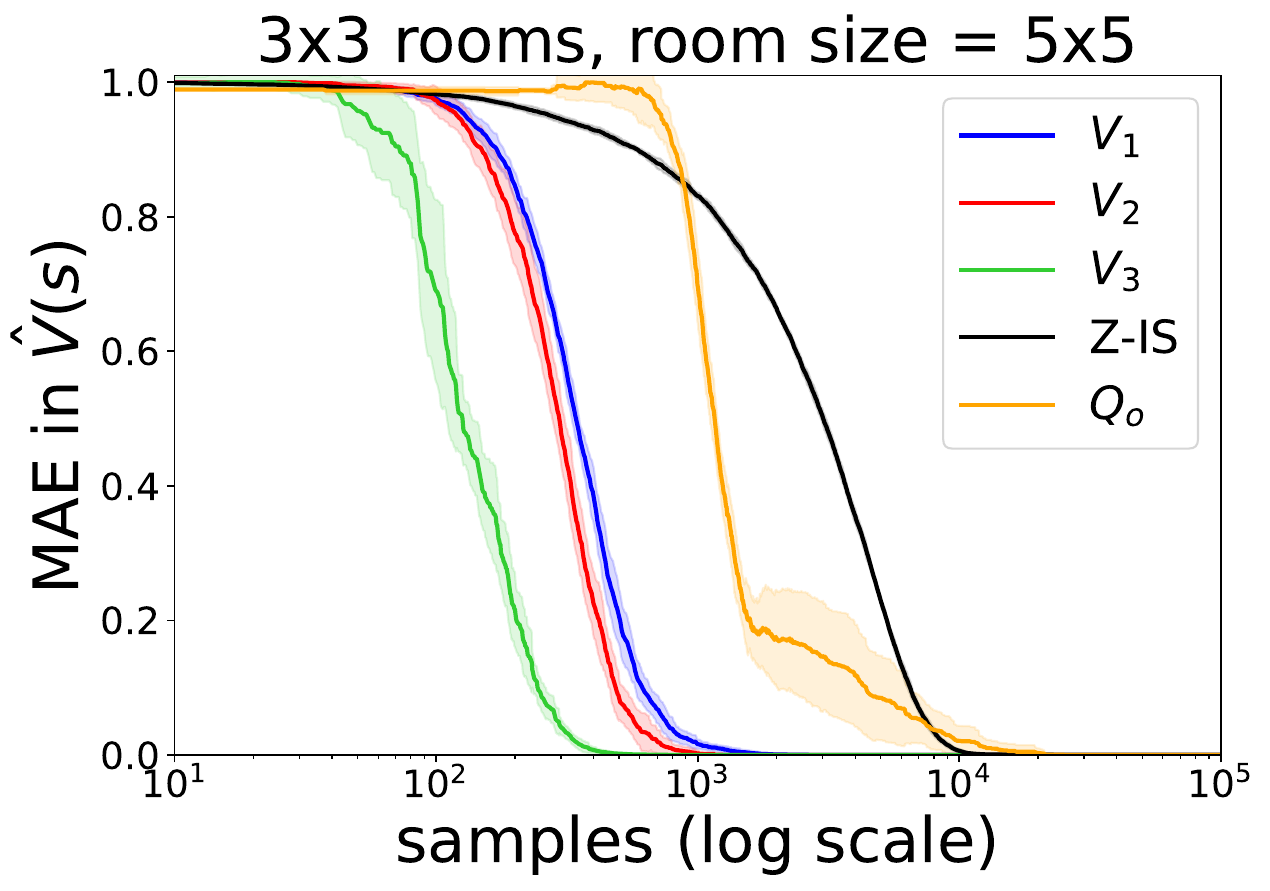
\includegraphics[width=0.32\textwidth]{figures/chapter1/learning/nrooms_3_3.pdf}
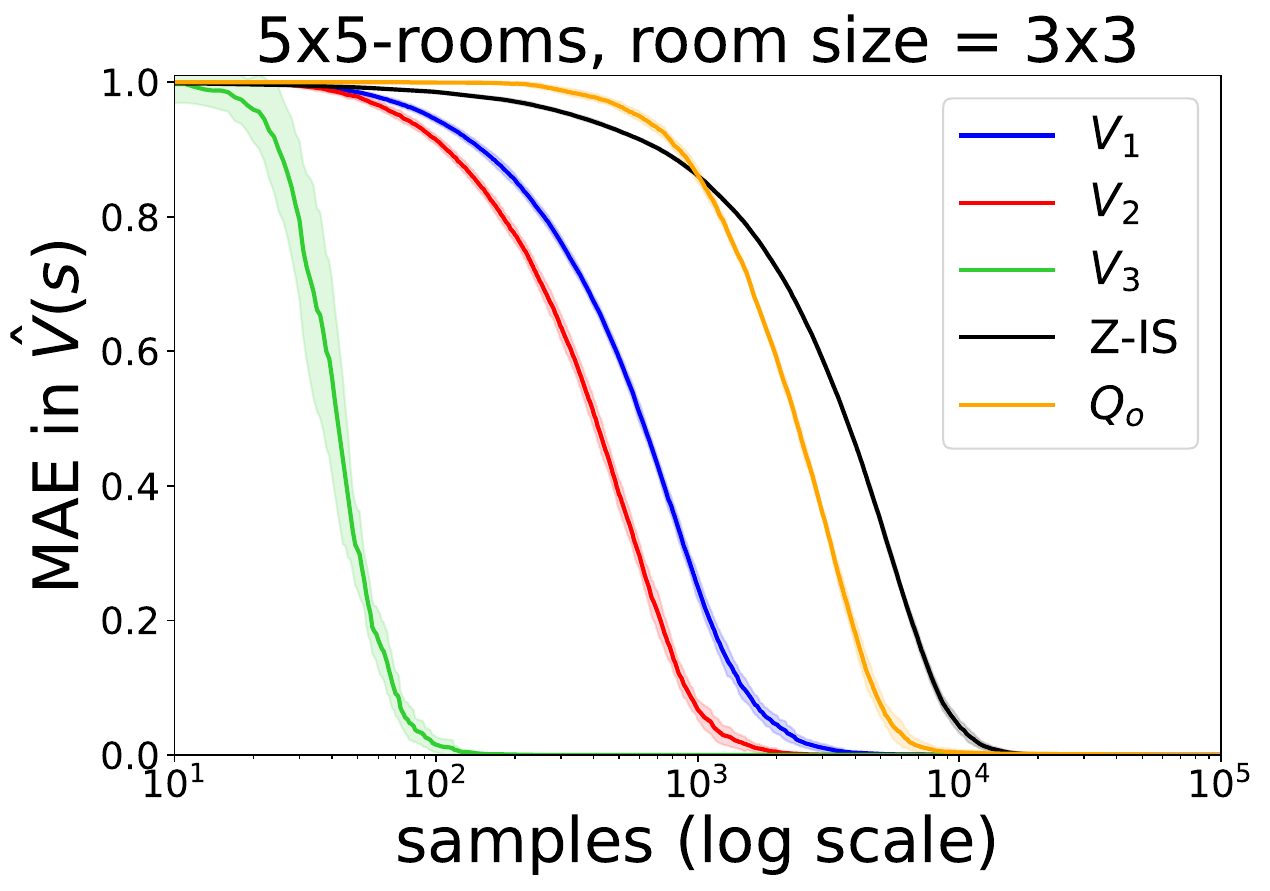
\includegraphics[width=0.32\textwidth]{figures/chapter1/learning/nrooms_5_5.pdf}
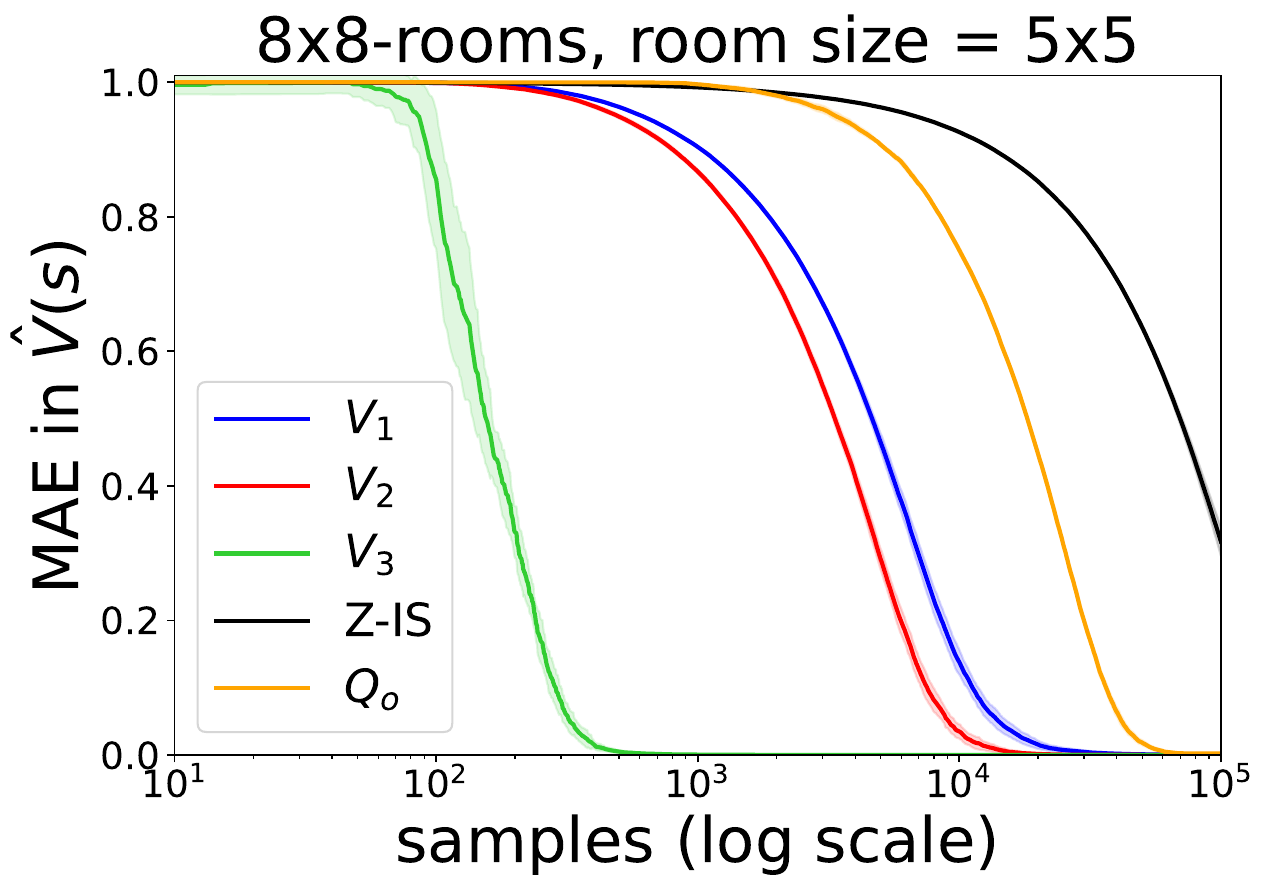
\includegraphics[width=0.32\textwidth]{figures/chapter1/learning/nrooms_8_8.pdf}
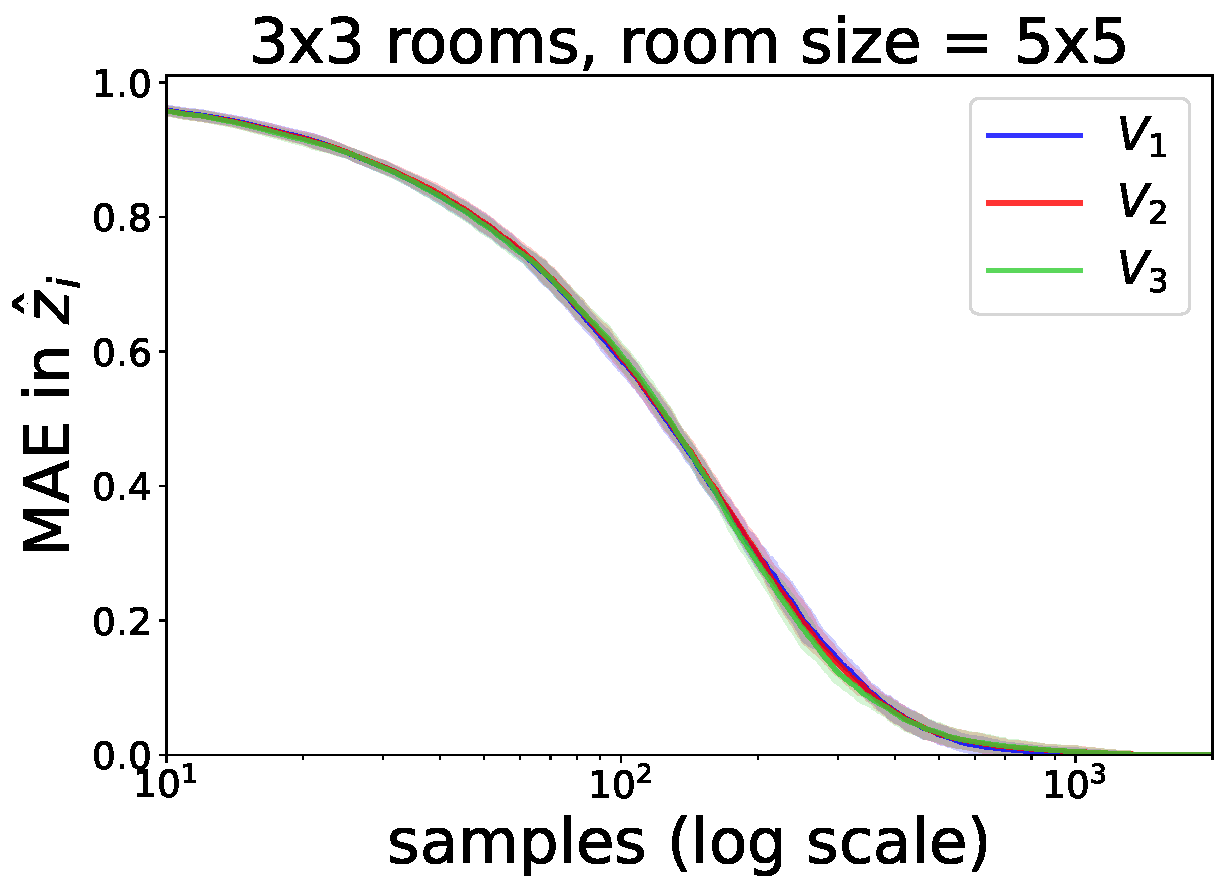
\includegraphics[width=0.32\textwidth]{figures/chapter1/subtasks/nrooms_3_3_subtasks.pdf}
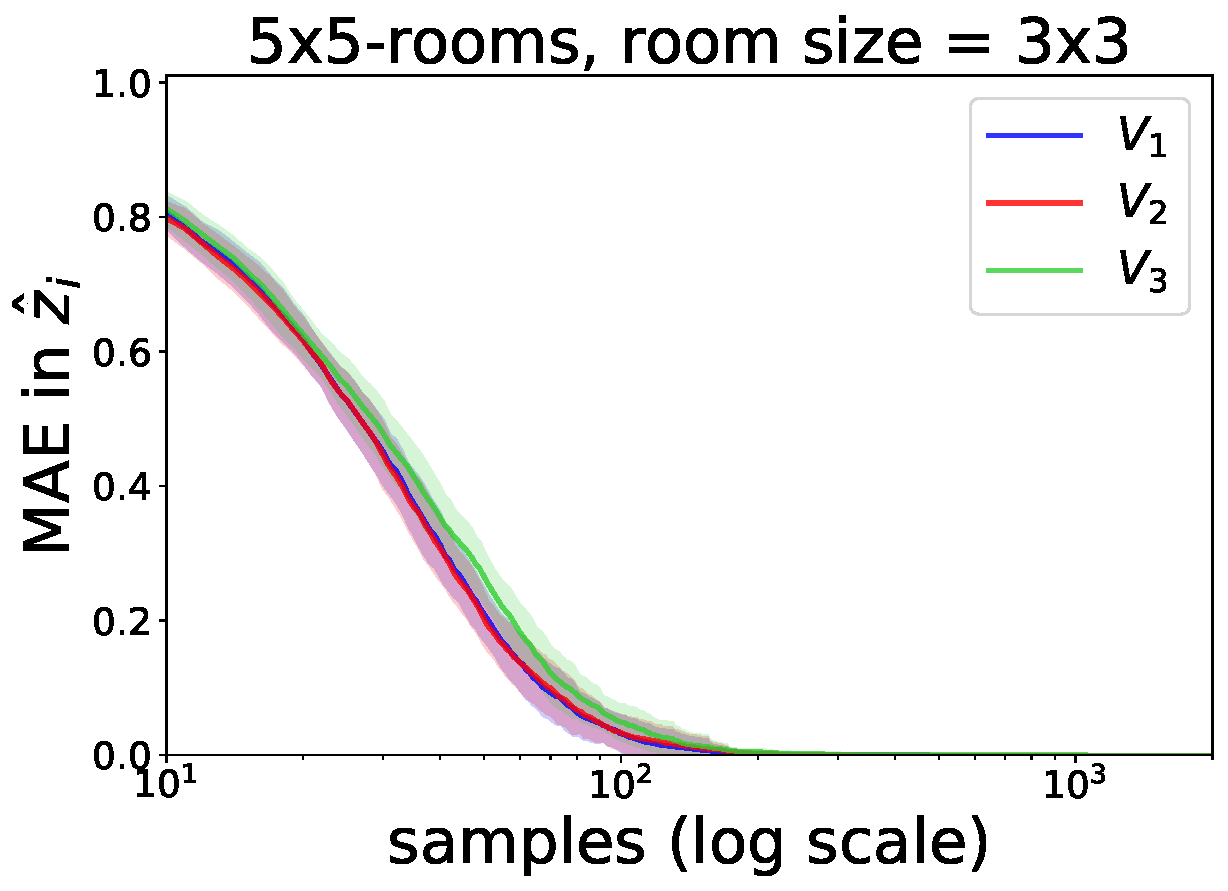
\includegraphics[width=0.32\textwidth]{figures/chapter1/subtasks/nrooms_5_5_subtasks.pdf}
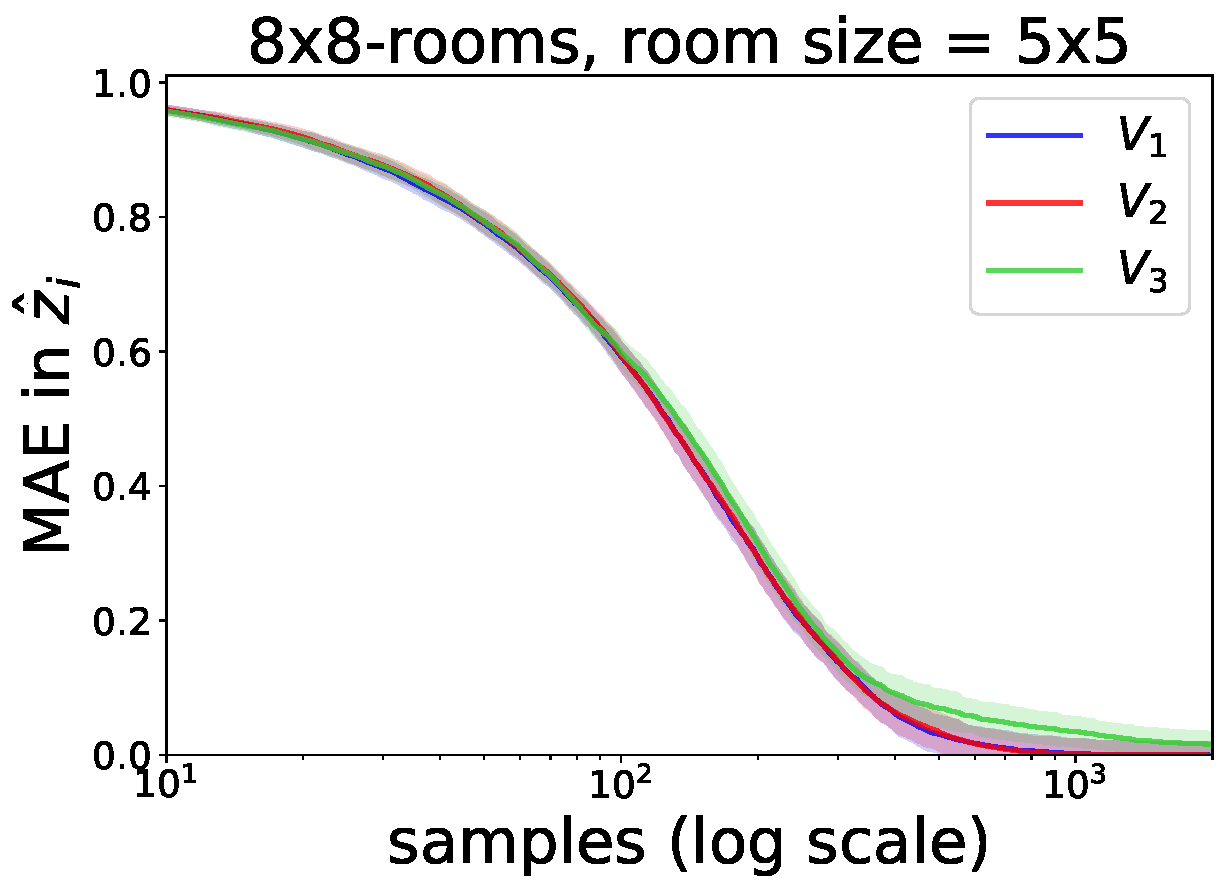
\includegraphics[width=0.32\textwidth]{figures/chapter1/subtasks/nrooms_8_8_subtasks.pdf}
\caption{ Results for $3\times 3$ rooms of size $5 \times 5$ (left);
$5\times 5$ rooms of size $3 \times 3$ (center); $8 \times 8$ rooms of size $5\times 5$ (right).}
%; and d) $5 \times 5$ with Q-learning ($Q_o$).}
\label{fig:hlmdps_errors_nrooms}
\end{figure}

Figure~\ref{fig:hlmdps_errors_nrooms} (left) shows results for $3\times 3$ rooms of size $5\times 5$ and Figure~\ref{fig:hlmdps_errors_nrooms} (center) shows results for $5\times 5$ rooms of size $3\times 3$. Both scenarios have $225$ interior states.
The difference between variants $V_1$, $V_2$ and $V_3$ is more pronounced in the second case, when the number of subtasks increases (more rooms) and the partition for each subtask is smaller (smaller rooms). Figure~\ref{fig:hlmdps_errors_nrooms} (right) shows how the method scales with the number of rooms of size $5\times 5$.
Again, variant $V_3$ has the best performance, in this case by a larger 
margin than before.

In all cases, the the convergence of the subtasks coincides almost exactly with the convergence of the higher level. This suggests that, once the agent has learned the value function for the subtasks, learning the value in the reduced number of exit states is an easy process due to compositionality. Surprisingly, the variant $V_3$ seems to converge before the subtasks do. This might be an effect of the choice of the metric used at the higher level, since only the error at the exit states is reported. It might be the case that, since exit states are pairwise contiguous, the algorithm does not need the value function for the whole subtask to be accurate, only at the required exit states. This phenomenom shoudl disapear if the MAE is taken over the whole state space instead.

% Vicenc:
%Figure~\ref{fig:hlmdps_errors_nrooms} (left) shows results for $3\times 3$ rooms of size $5\times 5$ and Figure~\ref{fig:hlmdps_errors_nrooms} (center) shows results for $5\times 5$ rooms of size $3\times 3$. Both scenarios have $225$ interior states.
%The difference between variants $V_1$, $V_2$ and $V_3$ is more pronounced in the second case, when the number of subtasks increases (more rooms) and the partition for each subtask is smaller (smaller rooms). Figure~\ref{fig:hlmdps_errors_nrooms} (right) shows results for a larger number of rooms of size $5\times 5$. The variant $V_3$ has the best performance, in this case by a larger margin than before.



% Variant $V_3$, updating the exits of all equivalent rooms, converges the fastest, and the difference increases as a function of the number of rooms.

%We run several experiments with different grid sizes. One one side, we kept the room dimensions fixed to $5 \times 5$ to analyze the impact of the number of rooms in two grids of $3 \times 3$ ($246$ states) and $8 \times 8$ ($1696$ states). Alternatively, we reduced the size of individual rooms to $3\times3$ and increased the number of rooms to $5 \times 5$ ($270$ states). The first and the last instances have the same number ($225$) of interior states. This allows us to have a better understanding of different  hierarchical structures.

%In each problem, we run the three variants of the model-free algorithm ($V_1$, $V_2$, $V_3$) and Z-learning without hierarchical decomposition (Z-IS). 


\subsection{Taxi Domain.}
%Since LMDPs have no explicit actions, we adapted the Taxi domain as follows.
To allow comparison between all the methods, we adapt the Taxi domain (see Figure~\ref{fig:domain_taxi}) as follows: when the taxi is at the correct pickup location, it can transition to a state with the passenger in the taxi.
In a wrong pickup location, it can instead transition to a terminal state with large negative reward (simulating an unsuccessful pick-up).
When the passenger is in the taxi, it can be dropped off at any pickup location, successfully completing the task whenever dropped at the correct destination.

\begin{figure}[!h]
\centering
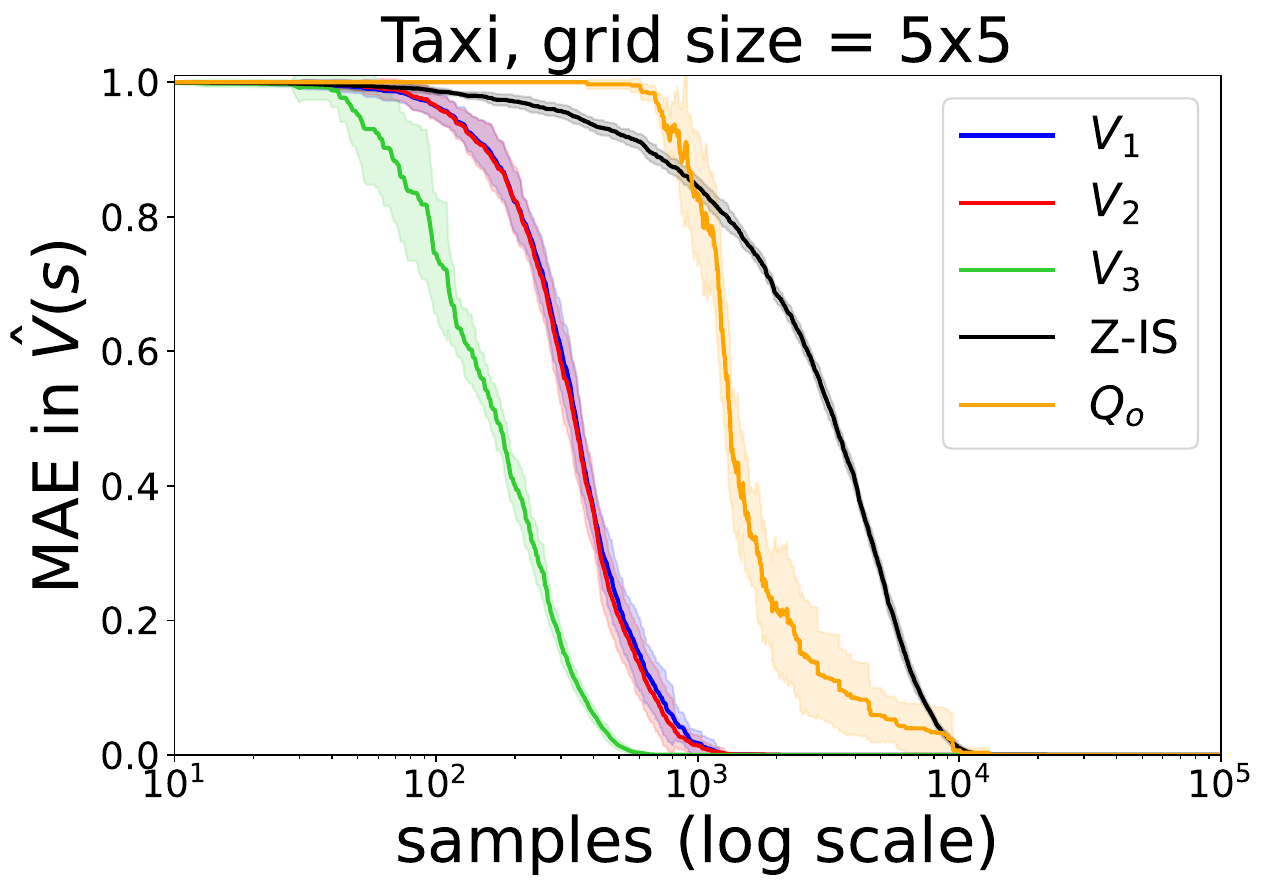
\includegraphics[width=0.49\textwidth]{figures/chapter1/learning/taxi_5.pdf}
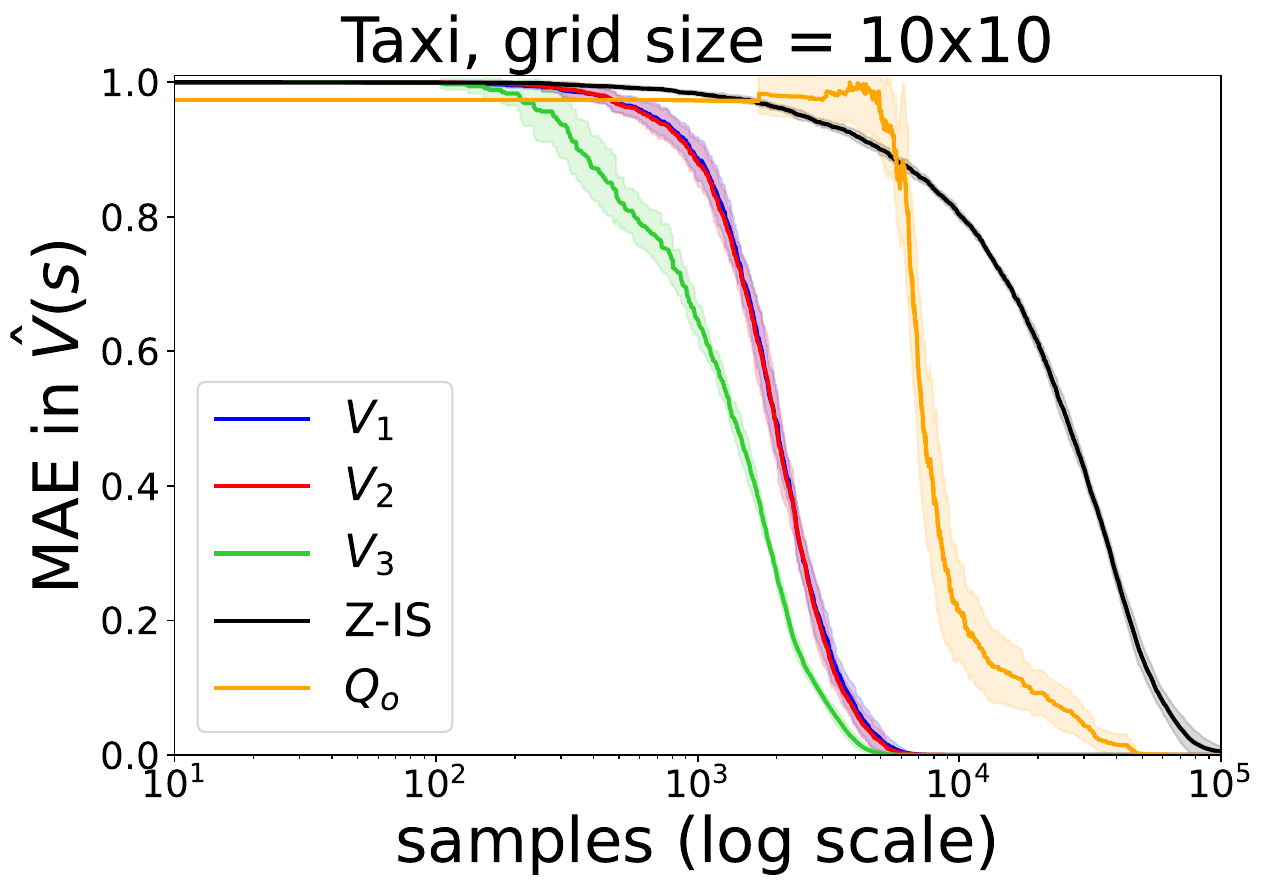
\includegraphics[width=0.49\textwidth]{figures/chapter1/learning/taxi_10.pdf}
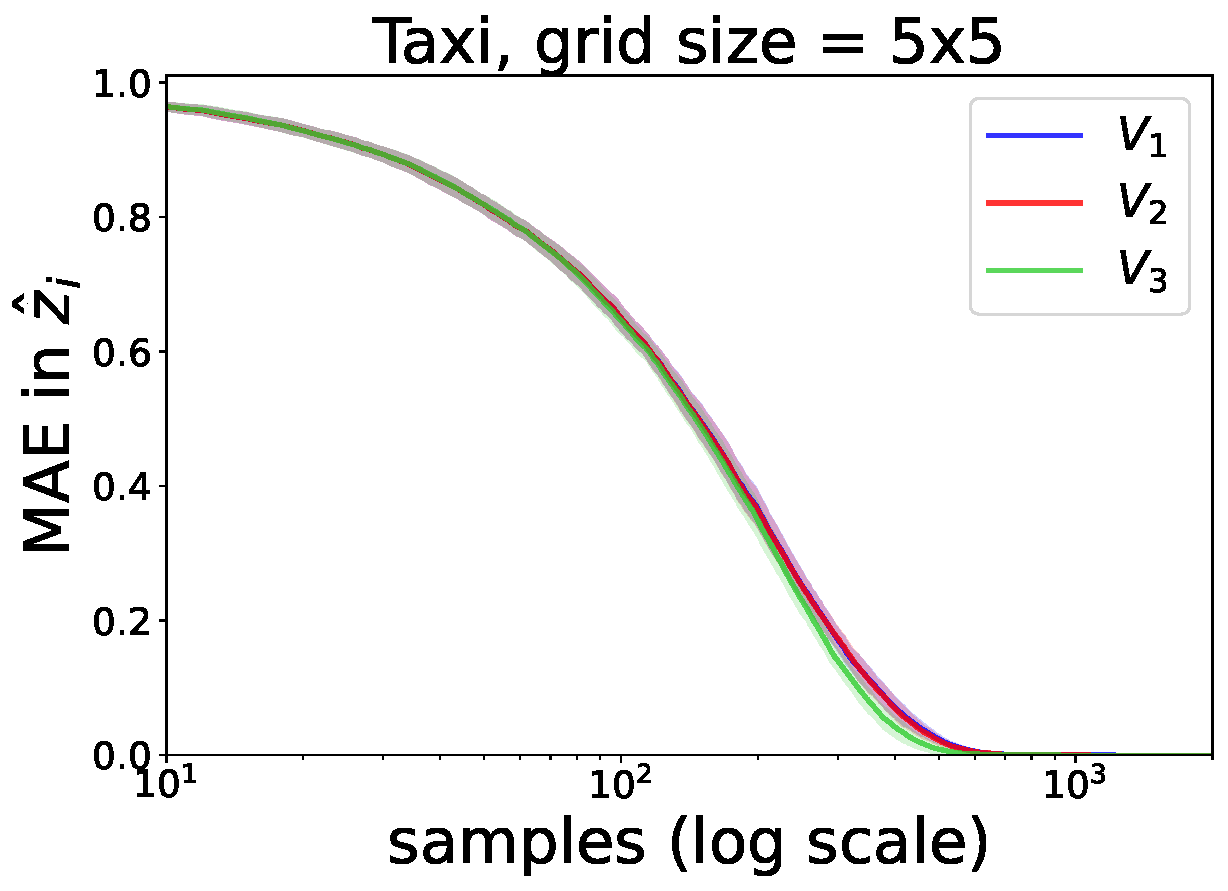
\includegraphics[width=0.49\textwidth]{figures/chapter1/subtasks/taxi_5_subtasks.pdf}
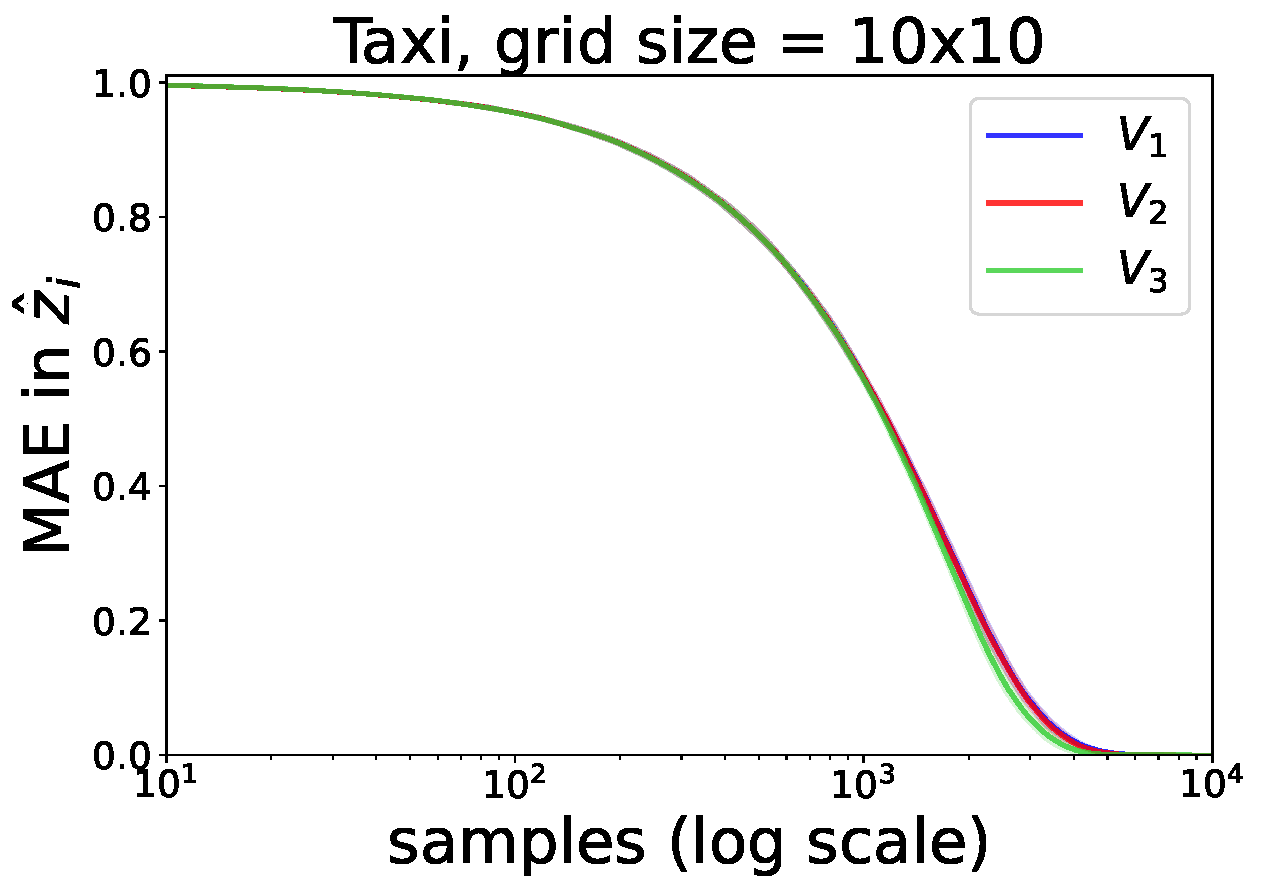
\includegraphics[width=0.49\textwidth]{figures/chapter1/subtasks/taxi_10_subtasks.pdf}
\caption{Results for $5 \times 5$ (left) and $10 \times 10$ (right) grids of Taxi domain.}
\label{fig:hlmdps_errors_taxi}
\end{figure}

%\begin{figure}[H]
%\centering
%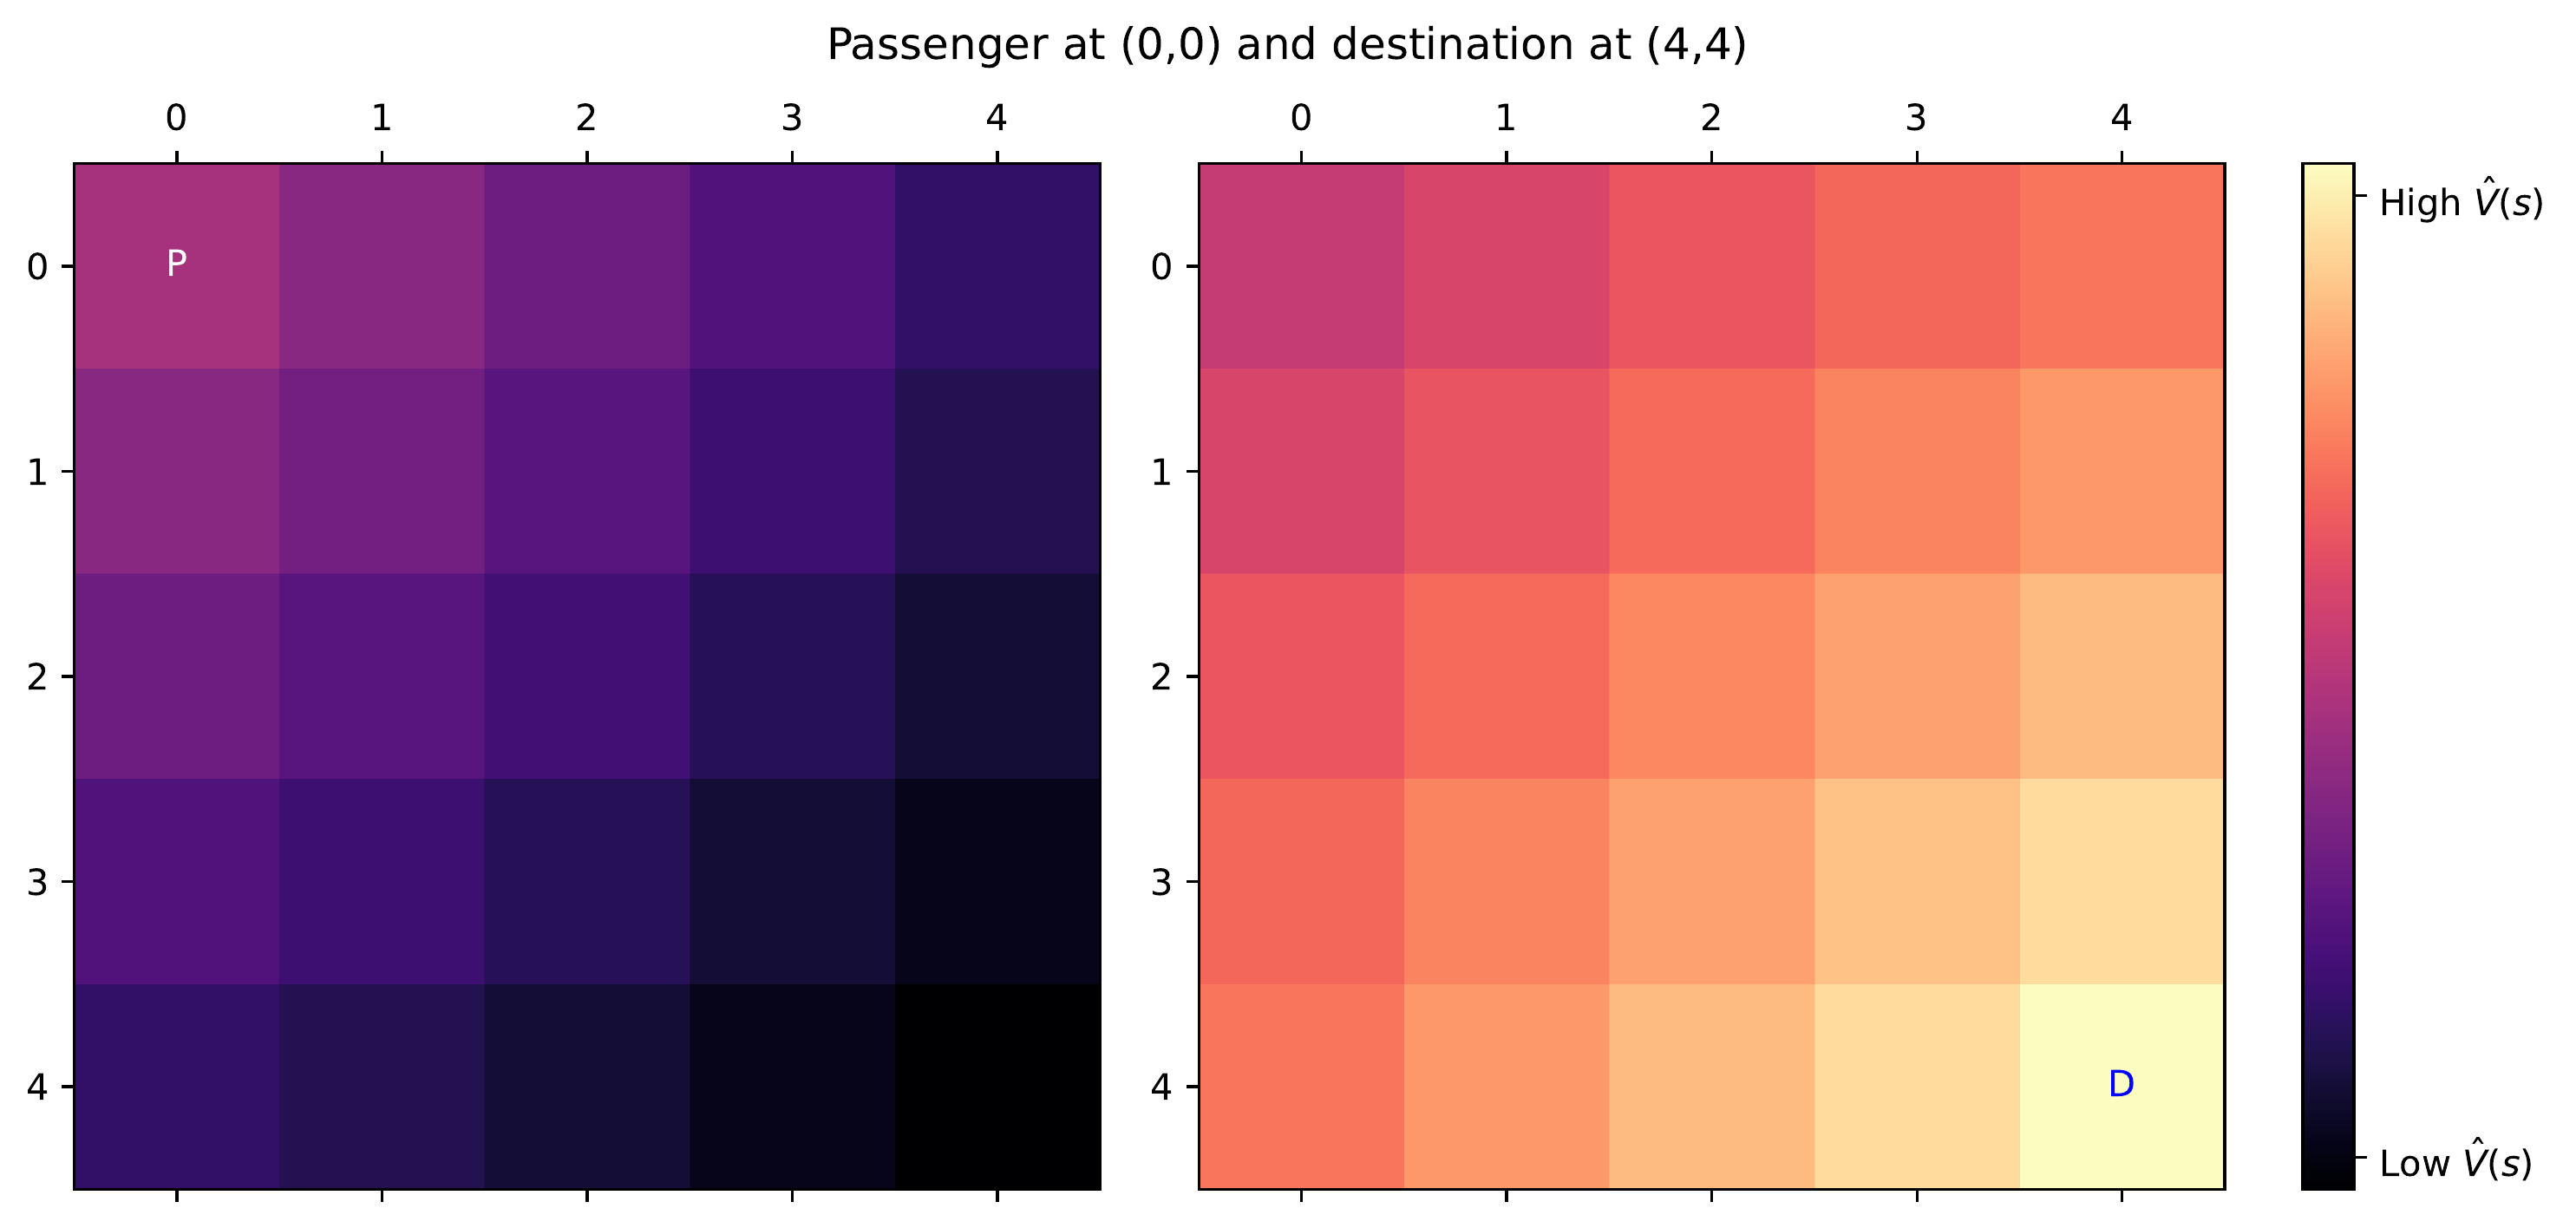
\includegraphics[scale=0.3]{Figures/taxi_dom_VF.png}
%\caption{$\widehat v(s)$ in a $5 \times 5$ Taxi, passenger (\textit{P}) and destination (\textit{D}).}
%\label{fig:taxi_VF}
%\end{figure}

%the pickup corner is an exit state connected to the partition in which the passenger is on the taxi (and, thus, can be moved to the destination) while the other corners are non-goal terminal states. This way, the agent can drop the passenger at any corners, but it will only successfully terminate the episode in the specified destination. If we disentangle the state space we can represent the value function graphically as in figure \ref{fig:taxi_VF}. In this domain, subtasks are to optimally go to the corners.
%\vspace{-0.1em}
Figure~\ref{fig:hlmdps_errors_taxi} shows results in two instances of size $5 \times 5$ ($408$ states) and $10 \times 10$ ($1608$ states). %, respectively.
Again, the proposed hierarchical approach outperforms Z-IS and $Q_o$.
In this case, the difference between $V_1$, $V_2$ and $V_3$ is less pronounced, even when the grid size increases, even though $V_3$ shows slightly better convergence. One possible explanation is the small number of exit states in this problem.

Again, the subtasks of the higher level converge in the same order of magnitud as the subtasks.


%Figures \ref{fig:hlmdps_errors_nrooms} and \ref{fig:hlmdps_errors_taxi} show the Mean Absolute Error (MAE) measured on $\widehat v(s)$ against the optimal value function $v^*(s)$ previously computed using the power iteration method. Clearly, our approach outperforms the flat version of Z-learning. Regarding the gridworld domain (figure \ref{fig:hlmdps_errors_nrooms}) it is observed that the three variants of our algorithm perform similarly for the case of the $3\times3$ grid. However, when the number of rooms is increased ($5\times5$ and $8\times8$ ) and thus, the hierarchical structure can be better exploited, each of the more sophisticated approaches improves the previous one. As for the Taxi domain (figure \ref{fig:hlmdps_errors_taxi}) the three versions converge much faster than flat learning, but yield similar results. In this case, the structure of the partitions (most of them have a single exit state) is the reason that further assumptions do not necessarily improve the performance as the three variants comprise the same effects.

\section{Discussion and Conclusion}

In summary, this chapter introduces a novel approach to hierarchical reinforcement learning that focuses on the class of linearly-solvable Markov decision processes.
Using subtask compositionality, the value function can be effectively decomposed and new hierarchical algorithms can be derived so that they converge to the optimal value function.
To the best of our knowledge, this approach is the first to exploit both the concurrent compositionality enabled by LMDPs together with hierarchies and intra-task learning to obtain globally optimal policies efficiently.

The proposed hierarchical decomposition leads to a new form of zero-shot learning that allows to incorporate subtasks that belong to an existing equivalent class without additional learning effort.
For example, adding new rooms in our example.
This is in contrast with existing methods that only exploit linear compositionality of tasks.

Our approach is limited to OR compositionality of subtasks, but there is no fundamental limitation that prevents arbitrary compositions.
The benefits of hierarchies can be combined for example, with the extended value functions proposed in~\citep{NangueTasse2020}.
\chapter{Hierarchical Average-reward Linearly-solvable Markov Decision Pocesses}
\section{Introduction}

Most previous work on hierarchical RL considers either the finite-horizon setting or the infinite-horizon setting with discounted rewards.
The average-reward setting is better suited for cyclical tasks characterized by continuous experience.
In the few works on hierarchical RL in the average-reward setting, either the low-level tasks are assumed to be solved beforehand~\citep{Fruit2017,Fruit2017b,Wan2021a} or they % low-level tasks 
have important restrictions that severely reduce their applicability, e.g.~a single initial state~\citep{Ghavamzadeh2007}. It is therefore an open question how to develop algorithms for hierarchical RL in the average-reward setting
%with the average-reward criterion
in order to learn the low-level and high-level tasks simultaneously.


In this Chapter we describe a novel framework for hierarchical RL in the average-reward setting that simultaneously solves low-level and high-level tasks. Concretely, considering the class of Linearly-solvable Markov Decision Processes (LMDPs)~\citep{Todorov2006}. The method here developed is an extension of the episodic case, described in the previous Chapter, to the average-reward setting. Even though the compositionality property for LMDPs or methods of similar flavor have been proposed in RL~\cite{Hunt2019,Niekerk2019,NangueTasse2020} and in combination with hierarchical RL in the finite-horizon setting~\cite{Jonsson2016,Saxe2017,Infante2022}, adapting this idea to the average-reward setting requires careful analysis and poses a new challenge.


%% VICEN
% LMDPs are a class of restricted MDPs for which the Bellman equation can be exactly transformed into a linear equation. This class of problems plays a key role in the framework of RL as probabilistic inference~\cite{Kappen2012,Levine2018}.
% One of the properties of LMDPs is compositionality: one can compute the solution to a novel task from the solutions to previously solved tasks without learning~\citep{Todorov2009a}. 
%In addition to many other properties, for LMDPs it is possible to compose a solution to a novel task from the solutions to previously solved task without learning~\citep{Todorov2009a}.


%%% PREVIOUS
% Since the Bellman optimality equations are linear for LMDPs, it is possible to compose a solution to a novel task from the solutions to previously solved task without learning~\citep{Todorov2009a}. Compositionality has been previously exploited for hierarchical reinforcement learning for LMDPs in the finite-horizon setting~\citep{Infante2022}, but adapting the idea to the average-reward setting requires careful analysis.

Similarly to the first-exit case and unlike most frameworks for hierarchical RL, this approach does not decompose the policy, only the value function. Hence the agent never chooses a subtask to solve, and instead uses the subtasks to compose the value function of the high-level task. 
This avoids introducing non-stationarity at the higher level when updating the low-level policies.

\section{Contributions}
In this Chapter we make the following contributions:
\begin{itemize}
  \item To develop a hierarchical framework that learns the low-level and  the high-level tasks simultaneously in the average-reward setting, without imposing additional restrictions on the low-level tasks.
    \item To propose two novel algorithms for solving hierarchical RL in the average reward setting: the first one is based on the eigenvector approach used for solving LMDPs. The second is an online variant in which an agent learns simultaneously the low-level and high-level tasks.
%  \item Representing low-level tasks as finite-horizon rather than average-reward decision processes.
    \item To provide two main theoretical contributions FOR LMDPs: convergence proofs for both differential soft TD-learning for (non-hierarchical) LMDPs and also for the eigenvector approach in the hierarchical case.
%  \item Proving the convergence of average-reward RL in non-hierarchical LMDPs.
  %\item Applying compositionality for reinforcement learning in the average-reward setting.
\end{itemize}

This work is the first that extends the combination of compositionality and hierarchical RL to the average-reward setting.

\section{Related work}
Most research on hierarchical RL formulates problems as a Semi-Markov Decision Process (SMDP) with options~\citep{Sutton1999} or the MAXQ decomposition~\citep{Dietterich2000}.

\citet{Fruit2017} and~\cite{Fruit2017b} propose algorithms for solving SMDPs with options in the average-reward setting, proving that the regret of their algorithms is polynomial in the size of the SMDP components, which may be smaller than the components of the underlying Markov Decision Process (MDP).
\citet{Wan2021a} present a version of differential Q-learning for SMDPs with options in the average-reward setting, proving that differential Q-learning converges to the optimal policy.
However, the above works assumes that the option policies are given prior to learning.
\citet{Ghavamzadeh2007} propose a framework for hierarchical average-reward RL based on the MAXQ decomposition, in which low-level tasks are also modeled as average-reward decision processes.
However, since the distribution over initial states can change as the high-level policy changes, the authors restrict low-level tasks to have a single initial state.

In the previous Chapter combine the compositionality of LMDPs with the equivalence of low-level tasks to develop a framework for hierarchical RL in the finite-horizon setting.

In contrast, our hierarchical framework based on LMDPs can represent the globally optimal policy.

\section{Alternative method for solving an ALMDP}

An alternative method for solving an ALMDP $\cL$ is to transform it to a first-exit LMDP. 
Given a reference state $s^*$ and an original ALMDP $\cL=\langle\cS,\kernel,\cR\rangle$, define a first-exit LMDP $\cL'=\langle\cS\setminus\{s^*\},\{s^*\}, \kernel',\cR',\cJ'\rangle$, where $\kernel'(s'|s)=\kernel(s'|s)$ for all state pairs $(s,s')\in(\cS\setminus\{s^*\})\times\cS$, and $\cJ(s^*)=0$ (implying $z(s^*)=1$). By inspection of~\eqref{eq:boe_z_lmdp} and~\eqref{eq:boe_z_almdp}, we observe that the Bellman optimality equation of $\cL'$ is identical to that of $\cL$ if $\cR'(s)=\cR(s)-\rho$. Even though the agent has no prior knowledge of the exponentiated gain $\Gamma = e^{\eta\rho}$, we perform binary search to find $\Gamma$. For a given estimate $\widehat\Gamma$ of $\Gamma$, after solving $\cL'$, $\widehat \Gamma z(s^*)$ is compared to $e^{\eta\cR(s^*)}\sum_s\kernel(s|s^*)z(s)$. If $\widehat \Gamma z(s^*)$ is greater, then $\widehat\Gamma$ is too large, else it is too small.

Alternatively, when $\kernel$ and $\cR$ are not known, an estimate $\widehat v$ of the optimal value $v$ and an estimate $\widehat\rho$ of the optimal gain $\rho$ are kept using \textit{differential soft TD-learning}, similar to differential Q-learning~\citep{Wan2021}. We collect $(s_t, r_t, s_{t+1})$ generated by the estimated policy $\widehat\pi$ derived from $\widehat v$ as in \eqref{eq:lmdp_optimal_policy}. The update rules for $\widehat v$ and $\widehat \rho$ from \eqref{eq:boe_almdp} are as follows
\begin{align}
    \widehat{v}_{t+1}(s_t) &\gets \widehat{v}_t(s_t) + \alpha_t \delta_t,
    \label{eq:halmdps_main_v_td_update}\\
    \widehat{\rho}_{t+1} &\gets \widehat{\rho}_t + \lambda \alpha_t \delta_t.\label{eq:halmdps_main_rho_td_update}
    \end{align}
Here, the TD error $\delta_t$ is given by
\begin{align*}
\delta_t &= r_t - \widehat{\rho}_t - \frac 1 \eta \log \frac {\widehat{\pi}_t(s_{t+1}|s_t)} {\kernel(s_{t+1}|s_t)} + \widehat{v}_t(s_{t+1}) - \widehat{v}_t(s_t)\\
 &= r_t - \widehat{\rho}_t + \frac 1 \eta \log \sum_{s'\in\cS} \kernel(s'|s_t) e^{\eta \widehat{v}_t(s')} - \widehat{v}_t(s_t).
\end{align*}
% The learning rates $\alpha_t$ and $\beta_t$ can be chosen independently.
Note that both updates use the same TD error. At any time, we can retrieve the estimates of $\widehat z$ and $\widehat\Gamma$ by exponentiating $\widehat v$ and $\widehat \rho$, respectively.


\begin{theorem}
    Under mild assumptions, differential soft TD-learning in~\eqref{eq:halmdps_main_v_td_update} and~\eqref{eq:halmdps_main_rho_td_update} converges to the optimal values of $v$ and $\rho$ in $\cL$. \label{theo:almdps}
\end{theorem}

\begin{proof}[Proof sketch]
The proof is adapted from the proof of convergence of differential Q-learning~\cite{Abounadi2001,Wan2021}, which requires the ALMDP to be communicating (Assumption~\ref{ass:communicating}).
Define a Bellman operator $T$ as
\[
T(v)(s) = \cR(s) + \frac 1 \eta \log \sum_{s'\in\cS} \kernel(s'|s) e^{ \eta v(s') }.
\]
To adapt the previous proof, it is sufficient to show that $T$ is a non-expansion in the max norm, i.e.~$\infnorm{T(x)-T(y)} \leq \infnorm{x - y}$ for each $x, y\in\real^{|\cS|}$, and that $T$ satisfies $T(x + c\mathds{1}) = T(x) + c\mathds{1}$ for each $x\in\real^{|\cS|}$ and constant $c\in\real$, where $\mathds{1}$ is $|\cS|$-dimensional vector of all ones.
For completeness, the full proof appears in Appendix~\ref{proof:theo_almdps}.
\end{proof}


\begin{figure*}
  \begin{center}
  \begin{adjustbox}{width=0.4\textwidth}
    \begin{tikzpicture}
      \draw[step=0.4,thin,shift={(0.2,0.2)}] (0.8,0.8) grid (4.8,4.8);
      \draw[ultra thick] (1,1) rectangle (5,5);
      \draw[ultra thick] (3,1) -- (3,1.8);
      \draw[ultra thick] (3,2.2) -- (3,3.8);
      \draw[ultra thick] (3,4.2) -- (3,5);
      \draw[ultra thick] (1,3) -- (1.8,3);
      \draw[ultra thick] (2.2,3) -- (3.8,3);
      \draw[ultra thick] (4.2,3) -- (5,3);

      \draw[fill] (0.6,1.8) rectangle (1,2.2);
      \draw[fill] (0.6,3.8) rectangle (1,4.2);
      \draw[fill] (1.8,5) rectangle (2.2,5.4);
      \draw[fill] (1.8,0.6) rectangle (2.2,1);
      \draw[fill] (3.8,0.6) rectangle (4.2,1);
      \draw[fill] (5,1.8) rectangle (5.4,2.2);
      \draw[fill] (5,3.8) rectangle (5.4,4.2);
      \draw[fill] (3.8,5) rectangle (4.2,5.4);

      \draw[ultra thick] (4.2,4.2) rectangle (4.6,4.6);
      \draw[ultra thick] (3.8,2.6) rectangle (4.2,3.4);
      \draw[ultra thick] (1.8,2.6) rectangle (2.2,3.4);
      \draw[ultra thick] (2.6,3.8) rectangle (3.4,4.2);
      \draw[ultra thick] (2.6,1.8) rectangle (3.4,2.2);

      \node (R) at (1.2,4.8) {} ;
      \node (G) at (4.4,4.4) {\tiny $G$};
      \node at (2,3.2) {\tiny $3^T$};
      \node at (2,2.8) {\tiny $1^B$};
      \node at (4,3.2) {\tiny $4^T$};
      \node at (4,2.8) {\tiny $2^B$};
      \node at (2.8,4) {\tiny $2^L$};
      \node at (2.8,2) {\tiny $4^L$};
      \node at (3.2,4) {\tiny $1^R$};
      \node at (3.2,2) {\tiny $3^R$};

    %   \draw[step=0.4,thin,shift={(0.2,0)}] (8.799,1.999) grid (10.8,4);
    %   \draw[ultra thick] (9,3.2) -- (8.6,3.2) -- (8.6,2.8) -- (9,2.8) -- (9,2) -- (9.8,2);
    %   \draw[ultra thick] (9,3.2) -- (9,4) -- (9.8,4) -- (9.8,4.4) -- (10.2,4.4) -- (10.2,4);
    %   \draw[ultra thick] (10.2,4) -- (11,4) -- (11,3.2) -- (11.4,3.2) -- (11.4,2.8) -- (11,2.8);
    %   \draw[ultra thick] (9.8,2) -- (9.8,1.6) -- (10.2,1.6) -- (10.2,2) -- (11,2) -- (11,2.8);
    %   \draw[ultra thick] (10.2,3.2) rectangle (10.6,3.6);

    %   \node at (10.4,3.4) {\small $G$};
    %   \node at (8.8,3)    {\small $L$};
    %   \node at (11.2,3)   {\small $R$};
    %   \node at (10,1.8)   {\small $B$};
    %   \node at (10,4.2)   {\small $T$};

    %   \node at (3,0.7) {\Large a)};
    %   \node at (10,0.7) {\Large b)};

      \draw [->] (G.north) to [out=100,in=120] (R.center);
    \end{tikzpicture}
  \end{adjustbox}
  \end{center}
  \caption{An example $4$-room ALMDP that shows the adaptation of the previously introduced N-room domain to the average-reward setting. \\}
  \label{fig:halmdps_example}
\end{figure*}

\section{Hierarchical Average-Reward LMDPs}

In this section we present our approach for hierarchical average-reward LMDPs. The idea is to take advantage of the similarity of the value functions in the first-exit and average-reward settings, and use compositionality to compose the value functions of the subtask LMDPs without additional learning.

%\subsubsection{Hierarchical Decomposition}
\subsection{Hierarchical Decomposition}
Consider an ALMDP $\langle\cS,\kernel,\cR\rangle$. Similarly to the previous Chapter, we assume the state space $\cS$ is partitioned into subsets $\left\{\cS_i\right\}^L_{i=1}$, with each partition $\cS_i$ inducing
a first-exit LMDP $\cL_i = \langle\cS_i, \cT_i, \kernel_i, \cR_i,\cJ_i\rangle$.
The components of each such subtask $\cL_i$ are defined as follows:
\begin{itemize}
  \item The set of states is $\cS_i$.
  \item The set of terminal states $\cT_i=\{\tau\in\cS\setminus\cS_i: \exists s\in\cS_i, \kernel(\tau|s)>0\}$ contains states not in $\cS_i$ that are reachable in one step from any state inside the partition.
  \item The transition function $\kernel_i$ and reward function $\cR_i$ are projections of $\kernel$ and $\cR-\widehat\rho$ onto $\cS_i$, where $\widehat\rho$ is a gain estimate.
  \item $\cJ_i$ is defined for each $\tau\in\cT_i$ as $\cJ_i(\tau)=\widehat v(\tau)$, where $\widehat v$ is a current value estimate (hence $z_i(\tau)=e^{\eta\widehat v(\tau)} = \widehat z(\tau)$ is defined by a current exponentiated value estimate $\widehat z$).
\end{itemize}
The Bellman optimality equations of each subtask $\cL_i$ are given by
\begin{equation}\label{eq:halmdps_subtask}
  z_i(s) = e^{\eta \cR_i(s)} \sum_{s'} \kernel_i(s'|s) z_i(s') \;\; \forall s\in\cS_i.
\end{equation}
By inspection of the Bellman optimality equations in~\eqref{eq:boe_z_almdp} and~\eqref{eq:halmdps_subtask}, they are equal if $\cR_i(s)=\cR(s)-\rho$. Thus, if $z_i(\tau)=z(\tau)$ for each $\tau\in\cT_i$ then the solution of the subtask $\cL_i$ corresponds to the optimal solution for each $s\in\cS_i$. However, in general neither $\rho$ nor $z(\tau)$ are known prior to learning and, therefore, estimates $\widehat\rho$ and $\widehat z(\tau)$ must be used instead. Each subtask $\cL_i$ can be seen as being {\it parameterized\/} on the value estimates $\widehat z(\tau)$ for each $\tau\in\cT_j$ and the gain estimate $\widehat\rho$. Every time that $\widehat z(\tau)$, $\tau\in\cT_i$, and $\widehat\rho$ change, we can obtain a new value estimate for each $s\in\cS_i$ by solving the subtask for the new parameters.

%\subsection{Subtask compositionality}
\subsection{Subtask Compositionality}
In the same way as in the first-exit case, it is impractical to solve each subtask $\cL_i$ every time the estimate $\widehat z(\tau)$ changes for $\tau\in\cT_j$. In order to alleviate this, we leverage compositionality for LMDPs. Again, the key insight is to build a basis of value functions that can be combined to obtain the solution for the subtasks.

Consider a subtask $\cL_i=\langle\cS_i,\cT_i,\kernel_i,\cR_i,\cJ_i\rangle$ and let $n=|\cT_i|$.  Let $\{\cL_i^1,\ldots,\cL_i^n\}$ be $n$ base LMDPs that are first-exit LMDPs and terminate in $\cT_i$. These base LMDPs only differ from $\cL_i$ in the reward of each terminal state $\tau^k\in\cT_i$. For all $s\in\cS_i$, the reward for each $\cL_i^k$ is by definition $\cR_i(s)=\cR(s)-\widehat\rho$ for all $s\in\cS_i$, while at terminal states $\tau\in\cT_i$ let the reward function is $z_i^k(\tau;\widehat\rho)=1$ if $\tau=\tau^k$ and $z_i^k(\tau;\widehat\rho)=0$ otherwise. Thus, the base LMDPs are parameterized by the gain estimate $\widehat\rho$. This is equivalent to setting the reward to $\cJ_i^k(\tau)=0$ if $\tau=\tau_k$ and $\cJ_i^k(\tau)=-\infty$ otherwise. Intuitively, each base LMDP solves the subtask of reaching one specific terminal state $\tau_k\in\cT_i$.

Assume that the solution $z_i^1(\cdot;\rho),\ldots,z_i^n(\cdot;\rho)$ for the base-LMDPs (for the optimal gain $\rho$) is available as well as the optimal value $z(\tau^k)$ of the original ALMDP for each terminal state $\tau^k\in\cT_i$. Then by compositionality we could represent the value function of each terminal state can be represented as a weighted combination of the subtasks:
\begin{equation}
  z(\tau) = \sum_{k=1}^n w_k z_i^k(\tau;\rho) =  \sum_{k=1}^n z(\tau^k) z_i^k(\tau;\rho) \;\;\forall\tau\in\cT_i.
  \label{eq:comp_terminal}
\end{equation}

Clearly, the RHS in the previous expression evaluates to $z(\tau)$ since $z(\tau^k) z_i^k(\tau;\rho) = z(\tau)\cdot 1$ when $\tau = \tau^k$, and
$z(\tau^k) z_i^k(\tau;\rho) = z(\tau^k)\cdot 0$ otherwise.

Thanks to compositionality, it is also possible to represent the value function for each subtask state $s\in\cS_i$ as
\begin{equation}
  z(s) = \sum_{k=1}^n z(\tau^k) z_i^k(s;\rho)\;\;\forall s\in\cS_i.
  \label{eq:halmdps_comp_internal}
\end{equation}
It is significant to remark that the base LMDPs depend on the gain $\rho$ by the definition of the reward function. This parameter is not known prior to learning. The subtasks in practice are solved for the latest estimate $\widehat\rho$ and must be re-learned for every update of this parameter until convergence.
\subsection{Efficiency of the value representation}
 Similar to previous work~\citep{Wen2020,Infante2022} the equivalence of subtasks is exploited to learn more efficiently. Let $\cC=\{\cC_1,\ldots,\cC_C\}$, $C\leq L$, be a set of equivalence classes, i.e.~a partition of the set of subtasks $\{\cL_1,\ldots,\cL_L\}$ such that all subtasks in a given partition are equivalent.
As before, a set of exit states as $\cE=\cup_{i=1}^L\cT_i$ is also defined.
Due to the decomposition, there is no need to keep an explicit value estimate $\widehat z(s)$ for every state $s\in\cS$. Instead, it is sufficient to keep a value function for exit states $\widehat z_\cE: \cE\rightarrow\real$ and a value function for each base LMDP of each equivalence class. This is enough to represent the value for any state $s\in\cS$ using the compositionality expression in~\eqref{eq:halmdps_comp_internal}.

Again, let $K=\max_{i=1} ^L\lvert\cS_i\rvert$,  $N=\max_{i=1} ^L\lvert\cT_i\rvert$ and $E=\lvert\cE\rvert$. Then only $O(KN)$ values are needed to represent the base LMDPs of a subtask, and the value function can be represented with $O(CKN + E)$ values. The decomposition leads to an efficient representation of the value function whenever $CKN + E \ll \lvert\cS\rvert$. This is achieved when there are few equivalence classes, the size of each subtask is small (in terms of the number of states) and there are relatively few exit states.

  % {\bf Example}: Consider the $4$-room example depicted in Figure~\ref{fig:halmdps_example}. Here there is a single equivalence class that generalizes all the rooms. Therefore, a single subclass is represented with $5\times 5$ states. This subtask induces $5$ base-LMDPs with terminal states in $G,L,R,T,B$. Besides, there is a total of 

  %{\bf Example 1:} 
  \begin{example}[Example 1]Figure~\ref{fig:halmdps_example} shows an 4-room LMDP adapted to the average-reward seeing. When reaching the state marked $G$, separate from the room but reachable in one step from the highlighted location, the agent receives a reward of $0$ and, in contrast to the first-exit case, the system transitions to a restart state (top left corner). In all other states the reward is $-1$. To behave optimally, thus, the agent should visit the state marked as $G$ as often as possible. The other aspects of the decomposition, remain equal to the first-exit setting. % as those of the subtasks.
  %Hence the number of equivalent subtasks is $C=1$, the number of non-terminal and terminal states of subtasks is $K=25$ and $N=5$, respectively, and the number of exit states is $E=9$.
    %In the 4-room example, t
    % There are five base LMDPs with value functions $z^G$, $z^L$, $z^R$, $z^T$ and $z^B$, respectively. Given an initial value estimate $\widehat{z}_\cE$ for each exit state in $\cE$, a value estimate of any state in the top left room is given by $\widehat{z}(s)=\widehat{z}_\cE(1^B) z^B(s) + \widehat{z}_\cE(1^R) z^R(s)$, where $\widehat{z}_\cE(G)=\widehat{z}_\cE(L)=\widehat{z}_\cE(T)=0$ is used to indicate that the terminal states $G$, $L$ and $T$ are not reachable in the top left room. 
    In this case, the total number of values needed to store the optimal value function is $E+CKN=9+125=134$, and the base LMDPs are faster to learn since they have smaller state space.
    %We need $CKN = 125$ values to store the value functions of the 5 base LMDPs, and $E=9$ values to store the value estimates of all exit states. Although this is more than the 100 states of the original LMDP, if we increase the number of rooms to $X\times Y$, the term $CKN$ is a constant as long as all rooms have equivalent dynamics, and the number of exit states is $E=(2X-1)(2Y-1)$, which is much smaller than the $25XY$ total states. For $10\times 10$ rooms, the value function decomposition requires $486$ values to represent the values of $2{,}500$ states.
  \end{example}

\section{Algorithms}
In this section we describe two novel algorithms for solving hierarchical ALMDPs. The first is a two-stage eigenvector approach that relies on first solving the subtasks. The second is an online algorithm in which an agent simultaneously learns the subtasks, the gain and the exit values from samples $(s_t, r_t, s_{t+1})$.
Once again it is important to remark that the values for states $s\notin\cE$ are not explicitly represented.

\subsection{Eigenvector approach}

In the episodic case, the base LMDPs are only solved once, and the solutions are then reused to compute the value function $z_\cE$ on exit states (see section~\ref{section:hlmdps_eigenvector_episodic}). However, in the case of ALMDPs, the reward functions of base LMDPs depend on the current gain estimate $\widehat\rho$, which is initially unknown. 

% I think the duration part is false!!!

%If we could estimate the expected {\em duration} $d_i(s)$ of each subtask $\cL_i$ from each state $s\in\cS_i$, we could use the duration to adjust the value estimate $\widehat z(s)$ of $s$ according to the current gain estimate $\widehat\Gamma$ by a factor $\widehat \Gamma^{d_i(s)}$. The duration can be recursively defined as $d_i(\tau)=0$ for each $\tau\in\cT_i$ and
%\[
%d_i(s) = 1 + \sum_{s'} \pi_i(s'|s) d_i(s').
%\]
%However, even though the subtask policy $\pi_i$ can be expressed in terms of the base LMDP policies $\pi_i^k$, we have been unable to formulate $d_i$ as a composition of the durations $d_i^k$ of base LMDPs, and hence the duration would have to be recomputed each time we resolve a subtask $\cL_i$, which is inefficient.

%We describe in Algorithm~\ref{alg:halmdps_eigenvector}. 
The eigenvector approach for solving hierarchical ALMDPs appears in Algorithm~\ref{alg:halmdps_eigenvector}. The intuition is that in each iteration, we first solve the subtasks for the latest estimate of the exponentiated gain $\widehat\Gamma$. For this, the base LMDPs are solved with~\eqref{eq:halmdps_subtask} using with the current value of $\widehat\rho$. Then~\eqref{eq:halmdps_comp_internal} is applied, restricted to $\cE$ to obtain an estimate of the value for the exit states. This yields the system of linear equations
\begin{equation}
    {\bf z_\cE} = G_\cE {\bf z_\cE}.\label{eq:halmdps_eigenvector}
\end{equation}
Here, the matrix $G_\cE\in\real^{\lvert\cE\rvert\times \lvert\cE\rvert}$ contains the optimal values of the base LMDPs and has elements defined as in~\eqref{eq:halmdps_comp_internal}. The previously introduced idea to transform the ALMDP $\cL$ to a first-exit LMDP $\cL'$ parameterized on the estimated gain $\widehat\rho$ is used, and the optimal exponentiated gain $\Gamma$ is found using binary search. There is a reference state $s^*\in\cS$ (which is by definition an exit state) and on which binary search is performed to find $\Gamma$.

\begin{algorithm}[!b]
  \caption{Eigenvector approach to solving a hierarchical ALMDP.}
  \setstretch{1.2}
  \begin{algorithmic}[1]
    %\Require{An ALMDP $\cL=\langle\cS,\cP,\cR\rangle$, a partition $\cS_1,\ldots,\cS_L$ of $\cS$, inducing a set of exit states $\cE$, reference state $s^\star$.}

    %\Procedure{\textsc{SolveALMDP}}{$\cL,\cS_1,\ldots,\cS_L,\cE,\epsilon,\eta$}
    \State{{\bf Input:} $\cL,\cS_1,\ldots,\cS_L,\cE,\epsilon,\eta$}
    \State $\text{lo}\gets 0$, $\text{hi}\gets 1$
    \While {$\text{hi} - \text{lo} > \epsilon$}
    \State $\widehat\Gamma \gets (\text{hi} + \text{lo}) \mathbin{/} 2$
    %\For{each subtask $\cL_i$}
    %\State Form the matrix $G_i = G_j(\eta,\widehat{\Gamma}_k)$
    %\State Solve the Bellman optimality equation $\widehat{\bf z}_i = G_i\widehat{\bf z}_i^+$
    %\EndFor
    \State Solve base LMDPs $\cL_j^1,\ldots,\cL_j^n$ for each equivalence class $\cC_j$
    \State Form the matrix $G_\cE$ from the optimal value functions
    \State Solve the system of equations  ${\bf \widehat z_\cE} = G_\cE {\bf\widehat z_\cE}$
    \If {$ \widehat\Gamma \widehat z_\cE(s^*) > e^{\eta \cR(s^*)} \sum_{s\in\cS} \kernel(s\lvert s^*) \widehat z_\cE(s)$}
    \State $\text{hi}\gets \widehat\Gamma$
    \Else \State $\text{lo}\gets \widehat\Gamma$
    \EndIf
    \vspace*{3pt}
    \EndWhile
    \State \Return value functions of all base LMDPs, ${\bf \widehat z_\cE}$
    %\EndProcedure
  \end{algorithmic}
  \label{alg:halmdps_eigenvector}
\end{algorithm}

\begin{theorem}\label{thm:converge}
    Algorithm~\ref{alg:halmdps_eigenvector} converges to the optimal value function $z$ of $\cL$ as $\epsilon\to 0$.
\end{theorem}
% The proof of Theorem~\ref{thm:converge} appears in Appendix~\ref{proof:theo_h}.

First note that the optimal value function $z$ of $\cL$ exists and is unique due to Assumption~\ref{ass:communicating}. Due to the equivalence between $\cL$ and the corresponding first-exit LMDP $\cL'$, this implies that $\cL'$ has a unique solution $z(\cdot;\rho)$ when the estimated gain $\widehat\rho$ equals $\rho$, and that this solution equals $z(\cdot;\rho)=z$, the optimal solution to $\cL$.

\begin{lemma}\label{lemma:monotonicity}
     Given a first-exit LMDP $\cL'$ parameterized on $\widehat\rho$, the optimal value $z(s;\widehat\rho)$ of each non-terminal state $s\in\cS$ is strictly monotonically decreasing in $\widehat\rho$.
\end{lemma}

\begin{proof}
Strict monotonicity requires that there exists $\varepsilon>0$ such that $\linebreak{z(s;\widehat\rho - \varepsilon) > z(s;\widehat\rho) > z(s;\widehat\rho+\varepsilon)}$ when $\varepsilon\rightarrow 0$. The first inequality is proven by induction; the second is analogous. The base case is given by the terminal states $\tau\in\cT$, for which $z(\tau;\widehat\rho - \varepsilon) = z(\tau;\widehat\rho)$. The inductive case is given by
\begin{align*}
    z(s;\widehat\rho-\varepsilon) &= e^{\eta(\cR(s) - (\widehat\rho -\varepsilon))}\sum_{s'\in\cS}\kernel(s'\lvert s) z(s';\widehat\rho- \varepsilon)\\
      &\geq e^{\eta\varepsilon} e^{\eta(\cR(s) - \rho))}\sum_{s'\in\cS}\kernel(s'\lvert s) z(s';\widehat\rho)\\
      &= e^{\eta\varepsilon} z(s;\widehat\rho) > z(s;\widehat\rho).
\end{align*}
This concludes the proof.
\end{proof}

As a consequence of Lemma~\ref{lemma:monotonicity}, $\cL'$ has a unique solution $z(\cdot,\widehat\rho)$ for each $\widehat\rho\geq\rho$, since the values $z(\cdot,\widehat\rho)$ decrease as $\widehat\rho$ increases. In contrast, there may be values of $\widehat\rho>\rho$ for which power iteration does not converge.

\begin{restatable}{lemma}{optimality}
Given a subtask $\cL_i$, if the optimal value of each terminal state $\tau\in\cT_i$ equals its optimal value in $\cL$, i.e. $z_i(\tau) = z(\tau)$, and the optimal gain $\rho$ in $\cL$ is known, then the optimal value of each non-terminal state $s\in\cS_i$ is unique and equals $z_i(s)=z(s)$.
    \label{lemma:optimality}
\end{restatable}

\begin{proof} Since $\cR_i$ and $\kernel_i$ are restrictions of $\cR-\rho$ and $\kernel$, respectively, to $\cS_i$, then
\begin{align*}
    z_i(s) &= e^{\eta\cR_i(s)}\sum_{s'}\kernel_i(s'\lvert s) z_i(s') = e^{\eta(\cR(s) - \rho)}\sum_{s'}\kernel(s'\lvert s) z_i(s'), \nonumber
\end{align*}
which is the same Bellman equation as for $z(s)$. Assuming that $z_i(\tau) = z(\tau)$ for each $\tau\in\cT$, directly yields that $z_i(s)=z(s)$ for each non-terminal state $s\in\cS_i$.
\end{proof}

\begin{corollary}\label{cor:uniqueness}
    If the optimal gain $\rho$ in $\cL$ is known, each base LMDP $\cL_j^k$ has a unique solution $z_j^k(\cdot;\rho)$.
\end{corollary}

\begin{proof} From \eqref{eq:halmdps_comp_internal}, the optimal values of subtask states satisfy
\[
  z(s) = \sum_{k=1}^n z(\tau^k) z_i^k(s;\rho)\;\;\forall s\in\cS_i.
\]
Due to Lemma~\ref{lemma:optimality}, the optimal value $z(s)$ is unique, which is only possible if $z_i^k(s;\rho)$ is unique for each $\tau^k\in\cT_i$.
\end{proof}

Combined with Lemma~\ref{lemma:monotonicity}, Corollary \ref{cor:uniqueness} implies that each base LMDP $\cL_j^k$ has a unique solution $z_j^k(\cdot;\widehat\rho)$ whenever $\widehat\rho\geq\rho$.

\begin{lemma}
For $\widehat\rho\geq\rho$, the equation ${\bf \widehat z_\cE} = G_\cE {\bf\widehat z_\cE}$ has a unique solution that equals $z_\cE(\tau)=z(\tau;\widehat\rho)$ for each exit $\tau\in\cE$, where $z(\cdot;\widehat\rho)$ is the unique value of the first-exit LMDP $\cL'$ for $\widehat\rho$.
\end{lemma}

\begin{proof}
At convergence, due to \eqref{eq:halmdps_comp_internal} it has to hold for each non-terminal exit $\tau\in\cE$ that
\[
  z_\cE(\tau) = \sum_{k=1}^n z_\cE(\tau^k) z_i^k(s;\widehat\rho)\;\;\forall s\in\cS_i,
\]
where each $\tau^k$ is also an exit and $z_i^k(s;\widehat\rho)$ is well-defined and unique since $\widehat\rho\geq\rho$. This equation is satisfied when $z_\cE(\tau)=z(\tau;\widehat\rho)$ for each exit. Since $z(\cdot;\widehat\rho)$ is unique, this is the only solution.
\end{proof}

Now we have all the ingredients to prove Theorem~\ref{thm:converge}. When $\widehat\rho\geq\rho$ (or equivalently, $\widehat\Gamma\geq\Gamma$), each base LMDP has a unique solution, and $z_\cE$ is also unique. Moreover, when $\widehat\rho>\rho$, the condition on line 8 is true, which causes binary search to discard all values greater than $\widehat\rho$. If the base LMDPs or $z_\cE$ do not have a unique solution, it means that $\widehat\rho$ is too small, and hence all values less than $\widehat\rho$ can be discarded. Since the solution $z(\cdot;\widehat\rho)$ is monotonically decreasing in $\widehat\rho$, binary search is guaranteed to find the optimal gain $\rho$ within a factor of $\epsilon$.

\subsection{Online hierarchical algorithm}
 In the online case (see Algorithm~\ref{alg:halmdps_online}), we keep an estimate of the exponentiated gain $\widehat\Gamma=e^{\eta\widehat\rho}$ which is updated every timestep. We also keep estimates of the value functions of the base LMDPs $\widehat z_i^1(\cdot;\widehat\rho),\ldots,\widehat z_i^n(\cdot;\widehat\rho)$ for each equivalence class $\cC_i$, and estimates of the value function on exit states $\widehat z_\cE$.  All the base LMDPs of the same equivalence class can be updated with the same sample using intra-task learning with the appropriate {\it importance sampling weights\/}~\citep{Jonsson2016}. We only update the estimates of the exit states upon visitation. In that case, the compositionality expression in~\eqref{eq:halmdps_comp_internal} is used to derive the following update:
\begin{equation}
  \widehat z_\cE(s)\gets (1-\alpha_\ell) \widehat z_\cE(s) + \alpha_\ell \sum_{k=1}^n \widehat z_\cE(\tau^k) \widehat z_i^k(s;\rho).
  \label{eq:halmdps_update_exit}
\end{equation}
Here, $\alpha_\ell$ is the learning rate. Each of the learned components (i.e., gain, base LMDPs and exit state value estimates) maintain independent learning rates.

\begin{algorithm}[!htpb]
  \caption{Online hierarchical algorithm.}
  \setstretch{1.12}
  \begin{algorithmic}[1]
    \State{{\bf Input:} $\cL,\cS_1,\ldots,\cS_L,\cE,s_0,\epsilon,\eta$}
    \State $t \gets 0$, $\widehat{\Gamma} \gets 1$
    \While {{\it not terminate}}
    \State Observe $(s_{t}, r_{t}, s_{t+1})\sim\widehat\pi_t$
    \State Update $\widehat z_j^1(\cdot;\widehat\rho),\ldots,\widehat z_j^n(\cdot;\widehat\rho)$ using Equation~\eqref{eq:halmdps_main_v_td_update}
    \State Compute $\widehat z(s_t)$ and $\sum_{s'}\kernel(s'|s_t)\widehat z(s')$ using Equation \eqref{eq:halmdps_comp_internal}
    \State Update $\widehat\Gamma$ using Equation~\eqref{eq:halmdps_main_rho_td_update}
    \If{$s_t\in\cE$}
    \State Update $\widehat z_\cE(s_t)$ using Equation~\eqref{eq:halmdps_update_exit}
    \EndIf
    \EndWhile
    \State \Return value functions of all base LMDPs, ${\widehat z_\cE}$

  \end{algorithmic}
  \label{alg:halmdps_online}
\end{algorithm}

\section{Experiments}

We now present the experimental results for the two benchmark control problems introduced in the previous Chapter and explain how we adapt them to the continuing case. \footnote{Code available at \url{https://github.com/guillermoim/halmdps}.}

We report some results for Algorithm~\ref{alg:halmdps_eigenvector}. These are  simple experiments meant to show that the hierarchical eigenvector method indeed converges to the optimal (exponentiated) gain up to an arbitrary precision, and, consequently, to the optimal value function.

Then, we compare Algorithm~\ref{alg:halmdps_online} against differential soft TD-learning in the flat representation of the ALMDP. Similarly to the first-exit case, the metric used for the experiments Mean Absolute Error (MAE) between the estimated value function $\widehat z$ and the true optimal value function $z$, taken exclusively at the exit states. For each algorithm, the results are averaged over five seeds. Along with the average, the standard deviation is also reported. Here, the learning rates decay every $n$ samples, and are given by the expression $\alpha_\ell \leftarrow k \alpha_\ell$, where $k$ is the decay factor. The hyperparameters $n$ and $k$ are optimized per instance. \todo{Why no $V_2$ and $V_3$.}

Note that, while the updates rules for differential Z-learning (Equations~\eqref{eq:diff_update_z} and~\eqref{eq:diff_update_gamma}) are in the exponential domain, the here derived soft TD-learning updates (Equations~\eqref{eq:halmdps_main_v_td_update} and~\eqref{eq:halmdps_main_rho_td_update}) are in the logarithmic domain. This has some advantages such as using a single TD-error for both the value function and the gain update. Similarly, for our hierarchical approach we can keep an estimate of the value function $\widehat v_{\cE}$ in the logarithmic domain. In such a case, the update rule~\eqref{eq:halmdps_update_exit} can be expressed as 
\begin{equation*}
    \widehat v_{\cE}(s)\gets (1-\alpha_\ell) \widehat v_\cE(s) + \alpha_\ell\frac{1}{\eta} \log\Big(\sum_{k=1}^n e^{\eta \widehat  v_\cE(\tau^k)} \widehat z_i^k(s;\rho)\Big).
\end{equation*}
Simultaneously, the gain estimate is updated with~\eqref{eq:halmdps_main_rho_td_update}. Recall that, at any moment, these estimates can be expressed in the exponential domain with $\widehat z_\cE(s)=e^{\eta\widehat v_\cE(s)}$ and $\widehat\Gamma=e^{\eta\widehat\rho}$. Our experimental results show that this version of the hierarchical algorithm is more stable.

\begin{figure}[!ht]
  \centering
  \includegraphics*[width=0.49\textwidth]{figures/chapter2/eigenvectors/lmdp-nroom-3.pdf}
  \includegraphics*[width=0.49\textwidth]{figures/chapter2/eigenvectors/lmdp-taxi-8.pdf}
  \caption{Error in $\widehat\Gamma$ per iteration for Algorithm~\ref{alg:halmdps_eigenvector}.}
  \label{fig:halmdps_eigenvectos}
 \end{figure}

Besides the learning error for the higher level, the learning error for the subtasks and the gain are also disclosed for the logarithmic and exponential domains. These results should be able to partly show better stability in the logarithmic domain. In contrast to the first-exit case, now there is a three-way dependency during learning between the (optimal) gain, value function of the subtasks and values of the exit states which makes hierarchical learning in the average-reward setting more challenging.  

  \subsection{N-room domain}
 As in the episodic case, there are some `goal' states with high reward (i.e. $0$). When the agent enters a goal state, the next action causes it to receive the given reward and transition to a {\it restart\/} location. The number of rooms as well as the size of the rooms are varied to obtain different instances of the problem.   
 
 Figure~\ref{fig:halmdps_eigenvectos} (left) shows the results for a single run of Algorithm~\ref{alg:halmdps_eigenvector} in the largest instance of this domain. We report the absolute error of the estimate $\widehat\Gamma$ at each iteration. We observe that the binary search procedure finds the optimal value up to an arbitrary precision which can be then used to compute the optimal value function. 
 
 The results for learning are in Figure~\ref{fig:halmdps_nrooms}. The difference in the error scale in the figures is due to the initialization of the base LMDPs. We observe that both the hierarchical approaches (logarithmic and exponential domains) outperfom the flat learner by several orders of magnitude (note the logarithmic scale).  The average reward setting poses an extra challenge since the `sparsity' of the reward can make the estimates of the gain oscillate. This ultimately has an impact on the estimates of the base LMDPs and the value estimates of the exit states, and it is likely the reason why in Figure~\ref{fig:halmdps_taxi} the error increases before decreasing down to zero. Nonetheless, the logarithmic version of the algorithm converges faster. This is likely to be caused by a faster convergence of $\widehat \Gamma$. The bottom row of Figure~\ref{fig:halmdps_nrooms} shows that the magnitude of this error behaves more stably in the logarithmic version, which might cause of the error in the subtasks (middle row of Figure~\ref{fig:halmdps_nrooms}) to be better upperbounded. Consequently, this might translate in a better convergence in the high-level (top row of Figure~\ref{fig:halmdps_nrooms}).

  \begin{sidewaysfigure}
  \centering
  \includegraphics*[width=0.32\textwidth]{figures/chapter2/online/nrooms_3_3_1.png}
  \includegraphics*[width=0.32\textwidth]{figures/chapter2/online/nrooms_5_5_1.png}
  \includegraphics*[width=0.32\textwidth]{figures/chapter2/online/nrooms_8_8_1.png}

  \includegraphics*[width=0.32\textwidth]{figures/chapter2/online/nrooms_3_3_subtasks_1.png}
  \includegraphics*[width=0.32\textwidth]{figures/chapter2/online/nrooms_5_5_subtasks_1.png}
  \includegraphics*[width=0.32\textwidth]{figures/chapter2/online/nrooms_8_8_subtasks_1.png}

  \includegraphics*[width=0.32\textwidth]{figures/chapter2/online/nrooms_3_3_gammas_1.png}
  \includegraphics*[width=0.32\textwidth]{figures/chapter2/online/nrooms_5_5_gammas_1.png}
  \includegraphics*[width=0.32\textwidth]{figures/chapter2/online/nrooms_8_8_gammas_1.png}


  \caption{Results in N-room when varying the number of rooms and the size of the rooms.}
  \label{fig:halmdps_nrooms}
  \end{sidewaysfigure}
  


  \subsection{Taxi domain}
  Adapting this environment to the continuing case is more natural. In this variant of the original domain~\citep{Dietterich2000}, once the passenger has been dropped off, the system transitions to a state in which the driver is in the last drop-off location, but a new passenger appears randomly at another location. Hence the driver immediately receives a new assignment after having successfully completed the previous one. 

  The results of the eigenvector algortihm in Figure~\ref{fig:halmdps_eigenvectos} (right) shows the same pattern as in the N-room domain. In this domain, the results for the learning algirthm Figure~\ref{fig:halmdps_taxi} also provide the same conclusions as in the N-room domain: the hierarhical approaches need less number of samples to converge, and the logarithmic version seems to be faster and more stable.



  \begin{figure}[!hb]
    \begin{center}
        \includegraphics*[width=0.49\textwidth]{figures/chapter2/online/taxi_5_1.png}
        \includegraphics*[width=0.49\textwidth]{figures/chapter2/online/taxi_8_1.png}
        \includegraphics*[width=0.49\textwidth]{figures/chapter2/online/taxi_5_subtask_1.png}
        \includegraphics*[width=0.49\textwidth]{figures/chapter2/online/taxi_8_subtask_1.png}
        \includegraphics*[width=0.49\textwidth]{figures/chapter2/online/taxi_5_gammas_1.png}
        \includegraphics*[width=0.49\textwidth]{figures/chapter2/online/taxi_8_gammas_1.png}
        % \includegraphics*[width=0.49\textwidth]{figures/chapter2/online/taxi_8_subtasks_1.pdf}
        \caption{Results for $5 \times 5$ (top) and $8 \times 8$ (bottom) grids of the Taxi domain.}
          \label{fig:halmdps_taxi}
    \end{center}
  \end{figure}
  %In this case, the adaptation to an infinite-horizon task is more natural. Once the passenger has been dropped off, the system transitions to a state in which the driver is in the last dropoff location, but a new passenger appears at another location. %Hence the driver immediately receives a new assignment after having successfully completed the previous one.

% \begin{figure*}[!bt]
%   \centering
%   \includegraphics*[width=0.32\textwidth]{pictures/nrooms_3_3-1.png}
%   \includegraphics*[width=0.32\textwidth]{pictures/nrooms_5_5-1.png}
%   \includegraphics*[width=0.32\textwidth]{pictures/nrooms_8_8-1.png}
%   \caption{ Results in N-room when varying the number of rooms and the size of the rooms.}
%   \label{fig:nrooms}
% \end{figure*}

% \begin{figure}[!htp]
%   \centering
%   \includegraphics*[width=0.33\textwidth]{pictures/taxi_5-1.png}
%   \includegraphics*[width=0.33\textwidth]{pictures/taxi_10-1.png}
%   \caption{Results for $5 \times 5$ (left) and $10 \times 10$ (right) grids of the Taxi domain.}
%   \label{fig:taxi}

% \end{figure}


\section{Conclusion}

In this Chapter we present a novel framework for hierarchical average-reward reinforcement learning which makes it possible to learn the low-level and high-level tasks simultaneously. 
We propose an eigenvector approach and an online algorithm for solving problems in our hierarchical framework, and show that the former converges to the optimal value function. We provide experimental results of the hierarchical updates both in the logarithmic and exponential domains that show that the logarithmic domain behaves more stably. The experimental results also show that either of the hierarchical versions outperforms a flat learner by several orders of magnitude.
As a by-product of our analysis, we also provide a convergence theorem in the non-hierarchical case for average-reward LMDPs, which to the extent of our knowledge, was not previously done. In the future we would like to prove convergence also for the proposed online algorithm.

\chapter{Compositionality with Successor Features via Policy Basis}
Autonomous agents that interact with an environment usually face tasks  that comprise complex, entangled behaviors over long horizons. Conventional reinforcement learning (RL) methods have successfully addressed this.  However, in cases when the agent is meant to perform several tasks across similar environments, training a policy for every task separately can be time-consuming and requires a lot of data. In such cases, the agent can utilize a method that has built-in generalization capabilities. One such method relies on the assumption that reward functions of these tasks can be decomposed into a linear combination of successor features~\citep{Barreto2017}. When a new task is presented, it is possible to combine previously learned policies and their successor features to solve a new task. %While the combination of such policies is guaranteed to be better than any previously learned policy, it need not be optimal.
While combining such policies is guaranteed to be an improvement over any previously learned policy, it may not necessarily be optimal. 
However, as shown by~\citep{Alegre2022}, %one can utilize recent advancement in multi-objective RL
one can leverage recent advancements in multi-objective RL to learn a set of policies that constitutes a policy basis to retrieve an optimal policy for any linear combination of successor features. 

While traditional RL methods rely on Markovian reward functions, defining a task using such a function can be challenging and sometimes impossible~\citep{Whitehead1995}. In scenarios where expressing the reward function in Markovian terms is not feasible, there has been a growing interest in alternative methods for task specification in recent years~\citep{Icarte2022, Camacho2019}. 
%While these and other conventional RL methods use Markovian reward functions, expressing a task with such reward function can be difficult and may not even be possible in some cases~\citep{Whitehead1995}. In settings where the reward function cannot be expressed in Markovian terms, task specification has raised especial interest in the last few years~\citep{Icarte2022, Camacho2019}.
In our work we focus on developing a method that utilizes generalization capabilities of successor features in a settings with non-Markovian reward functions.

Prior techniques for such settings have been proposed in contexts where a set of propositional symbols enables the definition of high-level tasks using logic~\citep{Vaezipoor2021, ToroIcarte2019}
%the existence of a set of propositional symbols allowed for the definition of high-level tasks by the means of logics~\citep{Vaezipoor2021, ToroIcarte2019}
or finite state automata (FSA)~\citep{Icarte2022}. Like in hierarchical RL,
%Similar to several hierarchical reinforcement learning methods, 
they are often based on decomposing tasks into sub-tasks and solving each sub-task independently~\citep{Dietterich2000, Sutton1999}. 
However, combining optimal solutions for sub-tasks may potentially result in a suboptimal overall policy. 
%While this has an advantage that solving parts of a task in isolation is often simpler, the disadvantage of such approach is that the combination of optimal solutions to sub-tasks can lead to a sub-optimal overall policy.
This is referred to as recursive optimality~\citep{Dietterich2000} or myopic policy~\citep{Vaezipoor2021}. 

To alleviate this issue, one can consider methods that condition the policy or the value function on the specification of the whole task~\citep{UVF} and such approaches were recently also proposed for tasks with non-Markovian reward functions \textit{Vaezipoor2021}. However, the methods that specify the whole task usually rely on a blackbox neural network for planning when determining which sub-goal to reach next. This makes it hard to interpret the plan to solve the task and although  they show promising results in practice, %they achieve promising empirical results 
it is unclear whether and when these approaches will generalize to a new task.

 % In this case, it is also possible to simplify the task description once a sub-goal has been achieved to improve the data efficiency and generalization. 

Instead, our work aims to use task decomposition without sacrificing global optimality to achieve predictable generalization. The method we propose learns a set of \textit{local} policies in sub-tasks such that their combination forms a \textit{globally optimal} policy for a large collection of problems described with FSAs. A new policy that solves any new task can then be created, without additional learning, by planning on a given FSA task description. Our contributions are:
 \begin{itemize}
    \item We propose to use successor features to learn a policy basis that is suitable for planning in stochastic domains.
    \item We develop a planning framework that uses such policy bases for zero-shot generalization to complex temporal tasks described by an arbitrary FSA.
    \item We prove that if the policies in this basis are optimal, our framework produces a globally optimal solution even in stochastic domains.
\end{itemize}



\section{Successor Features}

Successor features (SFs)~\citep{Dayan1993, Barreto2017} is a widely used RL representation framework that assumes the reward function is linearly expressible with respect to a feature vector,
\begin{equation}
  \cR^\w(s, a, s') = \w^\intercal\boldsymbol\phi(s, a , s').
  \label{eq:reward_sf}
\end{equation}

Here, $\boldsymbol\phi:\cS\times\cA\times\cS\rightarrow\real^{d}$ maps transitions to feature vectors and $\w\in\real^d$ is a weight vector. Every weight vector~$\w$ induces a different reward function and, thus, a task. The SF vector of a state-action pair $(s,a)\in\cS\times\cA$ under a policy $\pi$ is the expected discounted sum of future feature vectors: 
\begin{equation}
  \boldpsi^\pi(s, a) = \EEcp{\sum_{i=t}^\infty \gamma^{i-t} \boldsymbol\phi_i}{S_t = s, A_t = a}{\pi},
  \label{eq:sf}
\end{equation}
where $\boldsymbol\phi_i = \boldsymbol\phi(S_{i}, A_{i}, S_{i+1})$. The action value function for a state-action pair $(s, a)$ under policy $\pi$ can be efficiently represented using the SF vector. Due to the linearity of the reward function, the weight vector can be decoupled from the Bellman recursion. Following the definition of Equations~\eqref{eq:qfunction}~ and \eqref{eq:reward_sf}, the action value function in the SF framework can be rewritten as
\begin{align}
  Q^\pi_\w(s, a) &= \EEcp{\sum_{i=t} ^\infty \gamma^{i-t} \w^\intercal\boldsymbol\phi_i}{S_t = s, A_t = a}{\pi} \nonumber \\
                 & = \w^\intercal\EEcp{\sum_{i=t} ^\infty \gamma^{i-t} \boldsymbol\phi_i}{S_t = s, A_t = a}{\pi} \nonumber \\
                 &=  \w^\intercal \boldpsi^\pi(s, a) .
\label{eq:qfunction_sf}
\end{align}

The SF representation leads to \textit{generalized policy evaluation} (GPE) over multiple tasks~\citep{Barreto2020a}, and similarly, to \textit{generalized policy improvement} (GPI) to obtain new better policies~\citep{Barreto2017}.

A family of MDPs is defined as the set of MDPs that share all the components, except the reward function. This set is formally defined as 
\begin{equation*}
    \cM^{\boldsymbol{\phi}}\equiv\{\langle\cS,\cE,\cA,\cR_\w,\mathbb{P}_0, \mathbb{P},\gamma\rangle \lvert \cR_\w = \w^\intercal \boldsymbol{\phi}, \forall\w\in\real^d\}.
\end{equation*}

Transfer learning on families of MDPs is possible thanks to GPI. Given a set of policies $\Pi$, learned on the same family~$\cM^{\boldsymbol{\phi}}$, for which their respective SF representations have been computed, and a new task $\w'\in\real^d$, a GPI policy $\pi_{\text{GPI}}$ for any $s\in\cS$ is derived as 
\begin{equation}
    \pi_{\text{GPI}}(s) \in \argmax_{a\in\cA} \max_{\pi\in\Pi} Q^\pi_{\w'}(s, a).
    \label{eq:gpi}
\end{equation}

However, there is no guarantee of optimality for $\w'$.
A fundamental question to solve the so-called \textit{optimal policy transfer learning problem} is which policies should be included in the set of policies $\Pi$ so an optimal policy for any weight vector $\w\in\real^d$ can be obtained with GPI. 

\subsection*{Convex Coverage Set of Policies}

\begin{figure*}[!tb]
  %\centering
  \begin{subfigure}[t]{0.5\textwidth}
    \centering
    \begin{tikzpicture}[scale=0.6]
    % grid
    \draw[step=1cm,gray] (0,0) grid (10, 10);
    % walls
    \draw[ultra thick, fill=black] (5,10) -- (5, 3);
    \draw[ultra thick, fill=black] (1,5) -- (3, 5);
    \draw[ultra thick, fill=black] (7,5) -- (9, 5);

    % Symbols
    \node at (0.5,0.5) {\small $o^1$};
    \node at (0.5,7.5) {\small $\text{\mail}^2$};
    \node at (2.5,9.5) {\small $\text{\coffee}^1$};
    \node at (6.5,9.5) {\small $\text{\coffee}^2$};
    \node at (5.5,6.5) {\small $o^2$};
    \node at (9.5,0.5) {\small $\text{\mail}^2$};

    % agent
    \node at (3.5,1.5) {\small \agent};
    % Optimal path
    \draw[ultra thick, ->, >=stealth, draw=green!70!red!70] (3.5,1.9) -- (3.5,9.5) -- (2.9,9.5);
    \draw[ultra thick, ->, >=stealth, draw=green!70!red!70] (2.1,9.5) -- (0.5,9.5) -- (0.5,7.8) ;
    \draw[ultra thick, ->, >=stealth, draw=green!70!red!70] (0.5,7.2) -- (0.5,0.8);
    % Suboptimal path
     \draw[ultra thick, ->, >=stealth, draw=red!70!white] (3.8, 1.5) -- (8.5, 1.5) -- (8.5, 0.5) -- (9.1, 0.5);
     \draw[ultra thick, ->, >=stealth, draw=red!70!white] (9.5, 0.8) -- (9.5, 9.5) -- (6.9, 9.5);
     \draw[ultra thick, ->, >=stealth, draw=red!70!white] (6.1, 9.5) -- (5.5, 9.5) -- (5.5, 6.8);
    % \draw[ultra thick, ->, >=stealth, draw=blue!70!white] (2.5,1.9) -- (2.5,2.5) -- (1.5,2.5) -- (1.5,3.5) -- (2.5,3.5) -- (2.5,5.5) -- (1.5,5.5) -- (1.5,6.5) -- (2.5,6.5) -- (2.5,7.5) -- (3.5,7.5) -- (3.5,6.8);
    % \draw[ultra thick, ->, >=stealth, draw=blue!70!white] (3.8,6.5) -- (4.3,6.5) -- (4.3,4.8);

    % Outer box
    \draw[ultra thick] (0,0) rectangle (10,10);

\end{tikzpicture}


    \subcaption{}
    \label{fig:office_domain}
  \end{subfigure} 
  \hfill
  \begin{subfigure}[t]{0.5\textwidth}
    \centering
    
\begin{tikzpicture}[scale=0.29]
    % grid
    %\draw[step=1cm,gray] (0,0) grid (15, 15);
    % walls
    \fill[black] (0,0) rectangle ++ (3,3); 
    \fill[black] (4,0) rectangle ++ (3,3); 
    \fill[black] (8,0) rectangle ++ (3,3); 
    \fill[black] (12,0) rectangle ++ (3,3); 

    \fill[black] (0,4) rectangle ++ (3,3); 
    \fill[black] (4,4) rectangle ++ (3,3); 
    \fill[black] (8,4) rectangle ++ (3,3); 
    \fill[black] (12,4) rectangle ++ (3,3);

    \fill[black] (0,4) rectangle ++ (3,3); 
    \fill[black] (4,4) rectangle ++ (3,3); 
    \fill[black] (8,4) rectangle ++ (3,3); 
    \fill[black] (12,4) rectangle ++ (3,3);

    \fill[black] (0,8) rectangle ++ (3,3); 
    \fill[black] (4,8) rectangle ++ (3,3); 
    \fill[black] (8,8) rectangle ++ (3,3); 
    \fill[black] (12,8) rectangle ++ (3,3);

    \fill[black] (0,12) rectangle ++ (3,3); 
    \fill[black] (4,12) rectangle ++ (3,3); 
    \fill[black] (8,12) rectangle ++ (3,3); 
    \fill[black] (12,12) rectangle ++ (3,3);

    \fill[red] (1,7) rectangle ++ (1,1);
    \node at (1.5,7.5) {\color{white} A};
    \fill[blue] (3,13) rectangle ++ (1,1);
    \node at (3.5,13.5) {\color{white} C};
    \fill[olive] (11,3) rectangle ++ (1,1);
    \node at (11.5,3.5) {\color{white} B};
    \fill[purple] (7,1) rectangle ++ (1,1);
    \node at (7.5,1.5) {\color{white} H};

    % Symbols

    % agent
    % \node at (3.5,1.5) {\agent};
    % \draw[ultra thick, ->, >=stealth, draw=blue!70!white] (2.5,1.9) -- (2.5,2.5) -- (1.5,2.5) -- (1.5,3.5) -- (2.5,3.5) -- (2.5,5.5) -- (1.5,5.5) -- (1.5,6.5) -- (2.5,6.5) -- (2.5,7.5) -- (3.5,7.5) -- (3.5,6.8);
    % \draw[ultra thick, ->, >=stealth, draw=blue!70!white] (3.8,6.5) -- (4.3,6.5) -- (4.3,4.8);

    % Outer box
    \draw[ thick] (0,0) rectangle (15,15);

\end{tikzpicture}
    \subcaption{}
    \label{fig:delivery_domain}
  \end{subfigure}
  \hfill
  \caption{Depiction of the Office (a) and Delivery (b) environments, FSA task specification of the composite task in the Office domain and the FSA task specificiation of the sequential task in the Delivery domain (b). In (a) $\cP=\{\text{\coffee}, \text{\mail}, o\}$ and $\cE=\{\text{\coffee}^1,\text{\coffee}^2, \text{\mail}^1,\text{\mail}^2, o^1, o^2\}$. In (b), $\cE=\cP=\{A, B, C, H\}$.}
 \label{fig:domains}
\end{figure*}

The recent work of~\citep{Alegre2022} solves the optimal policy transfer learning problem. They draw the connection between the SF transfer learning problem and multi-objective RL (MORL). The pivotal fact is that the SF representation in Equation~\eqref{eq:sf} can be interpreted as a multidimensional value function and the construction of the aforementioned set of policies $\Pi$ can be cast as a multi-objective optimization problem.
 
 Consequently, the optimistic linear support (OLS) algorithm is extended with successor features in order to learn a set of policies that constitutes a \textit{convex coverage set} (CCS)~\citep{Roijers2015}. Their main result is the SFOLS algorithm (see Supplementary Material\footnote{Supplementary Material at {\texttt{\url{https://arxiv.org/abs/2403.15301}}}} for a full, technical description) in which a set $\Pi_\text{CCS}$ is built incrementally by adding (new) policies to such a set, until convergence. The set $\Pi_\text{CCS}$ contains all non-dominated policies in terms of their multi-objective value functions, where the dominance relation is defined over scalarized values ${V^\pi_\w = \mathbb{E}_{S_0\sim\mathbb{P}_0}\left[V^\pi_\w(S_0)\right]}$, and is characterized as
\begin{align}
  \Pi_\text{CCS} &= \{\pi\;\lvert\;\exists\w\;\text{s.t.}\;\forall {\boldpsi}^{\pi'},\; \w^\intercal {\boldpsi}^\pi {\;\geq\;} \w^\intercal{\boldpsi}^{\pi'} \} \nonumber\\
  &= \{ \pi \;\lvert\;\exists\w\;\text{s.t.}\;\forall {\pi'},\; {V^\pi_\w}{\;\geq\;} {V^{\pi'}_\w}\}.
\end{align} 
In every iteration $k$, SFOLS proposes a new weight vector $\w^k\in\Delta(d)$ for which an optimal policy (and its corresponding SF representation) is learned and added to $\Pi_\text{CCS}$ since it is sufficient to consider weights in $\Delta(d)$ to learn the full $\Pi_\text{CCS}$. The output of SFOLS is both $\Pi_\text{CCS}$ and the SF representation $\boldpsi^\pi$ for every $\pi\in\Pi_\text{CCS}$.
 
Intuitively, all policies in $\Pi_\text{CCS}$ are optimal in at least one task $\w \in \Delta(d)$.
The set $\Pi_\text{CCS}$ is combined with GPI, see Equation~\eqref{eq:gpi}, and upon convergence, for any (new) given task $\w'\in\real^d$, an optimal policy can be identified~\citep[cf. Theorem 2]{Alegre2022}.


\subsection{Propositional Logic}
We assume that environments are endowed with a set of high-level, boolean-valued propositional symbols $\cP$ and that they are associated with the set of exit states $\cE$ of a low-level MDP $\cM$. Every transition $\in\cS\times\cA\times\cS$ induces some propositional valuation (assignment of truth values) $2^\cP$. Such a valuation depends on the new state and occurs under a mapping ${\cO:\cS\rightarrow2^\cP}$ that is known to the agent. Nonetheless, only exit states $\varepsilon\in\cE$ make propositions true under $\cO$. We assume that that propositional symbols are mutually exclusive, and the agent cannot observe two symbols in the same transition. We say that a valuation $\Gamma$ satisfies a propositional symbol $p$, formally $\Gamma\vDash p$, if $p$ is true in $\Gamma$. 

\subsection{Finite State Automaton} Task instructions can be specified via a finite state automaton. These are tuples ${\cF=\langle \cU,u_0,\cT,L,\delta\rangle}$ where $\cU$ is the finite set of states, $u_0\in\cU$ is the initial state, $\cT$ is the set of terminal states with $\cU\cap\cT=\emptyset$, $L:\cU\times(\cU\cup\cT)\rightarrow 2^\cP$ is a labelling function that maps FSA states transitions to truth values for the propositions and $\delta:\cU\rightarrow \{0, 1\}$ is a high-level reward function. Each transition among FSA states $(u, u')$ defines a subgoal. The agent has to observe some propositional valuation $L(u, u')$ in order to achieve it and FSA states can only be connected by a subgoal. E.g., in Figure~\ref{fig:office_fsa_disjunction}, the FSA state $u_0$ has two outgoing subgoals: getting mail (labeled as \mail) and getting coffee (labeled as \coffee). Non-existing transitions $(u, u')$ get mapped to $L(u, u')=\bot$. The reward function $\delta$ gives a reward larger than 0 only to terminal states. In other words, such a reward function is $\delta(u)=0\;\forall u\in\cU$ and $\delta(\mathbf{t})=1\;\forall \mathbf{t}\in\cT$. 

\begin{figure}[!hbt]
  \centering
  \begin{subfigure}[h]{0.23\textwidth}
    \centering
    \begin{tikzpicture}[scale=0.54]

    % Outer box
    \draw[step=0.5cm,lightgray] (0,0) grid (8, 6);
    \draw[ultra thick] (0,0) rectangle (8,6);

    % agent
    \node at (0.3, 2.8) {\miniagent};
    % \draw[ultra thick, ->, >=stealth, draw=blue!70!white] (2.5,1.9) -- (2.5,2.5) -- (1.5,2.5) -- (1.5,3.5) -- (2.5,3.5) -- (2.5,5.5) -- (1.5,5.5) -- (1.5,6.5) -- (2.5,6.5) -- (2.5,7.5) -- (3.5,7.5) -- (3.5,6.8);
    % \draw[ultra thick, ->, >=stealth, draw=blue!70!white] (3.8,6.5) -- (4.3,6.5) -- (4.3,4.8);
    \draw[fill=blue] (7.5,5.5) --  (7.5,6) -- (8,6) -- (8,5.5) -- cycle;
    % Outer box
    \draw[fill=red]  (7.5,0) --  (7.5,0.5) -- (8,0.5) -- (8,0) -- cycle;

    % \node[color=white] at (7.5,5.5) {$\text{G}_1$};
    % \node[color=white] at (7.5,0.5) {$\text{G}_2$};

\end{tikzpicture}

    \caption{}
    \label{fig:office_fsa_disjunction}
  \end{subfigure}
  \hfill 
  \begin{subfigure}[h]{0.23\textwidth}
    \centering
    \begin{tikzpicture}[node distance=cm,on grid,every initial by arrow/.style={ultra thick,->, >=stealth}]
    \node[thick,state,initial above] (u_0) at (0,0) {$u_0$};
    \node[ thick,state]         (u_1) at (-0.7,-1.4)  {$u_1$};
    \node[ thick,state]         (u_2) at (0.7,-1.4)  {$u_2$};
    \node[ thick,state]         (u_3) at (-0.7,-3)  {$u_3$};


    \node[circle,draw=black,minimum size=0.26cm,inner sep=0pt,fill=black] (t3) at (0.9,-3)  {};
    \node[text width=1cm ] at (1.2,-2.7) {$u_T$};

    \path[thick,->, >=stealth] (u_0) edge node [left] {$A$} (u_1);
    \path[thick,->, >=stealth] (u_0) edge node [right] {$B$} (u_2);
    \path[thick,->, >=stealth] (u_1) edge node [left] {$C$} (u_3);
    \path[thick,->, >=stealth] (u_2) edge node [right] {$C$} (u_3);
    \path[thick,->, >=stealth] (u_3) edge node [below] {$H$} (t3);

\end{tikzpicture}
    \caption{}
    \label{fig:office_fsa_composite}
  \end{subfigure}
  \caption{Disjunction (a) and composite (b) FSA task specifications for the Office domain.}
 \label{fig:sample_fsas}
\end{figure} 

\section{Using Successor Features to Solve non-Markovian Reward Specifications}

We focus on the setting in which a low-level MDP is equipped with a reward structure like in Equation~\eqref{eq:reward_sf}. We let the low-level be represented by a family of MDPs $\cM^{\boldsymbol{\phi}}$, where each weight vector $\w\in\real^d$ specifies a low-level task. The agent receives high-level task specifications in the more flexible form of an FSA which permits the specification of non-Markovian reward structures. The combination of a low-level family of MDPs and a high-level FSA gives rise to a \textit{product MDP} $\cM'=\cF\times\cM^{\boldsymbol{\phi}}$ that satisfies the Markov property, and where the state space is augmented to be $\;\cU\times\cS$.

A product MDP $\cM'$ is a well-defined MDP. The agent now follows a policy $\mu:\cU\times\cS\rightarrow\Delta(\cA)$, that depends both on the FSA state and the underlying MDP state. $\cM'$ can be solved with conventional RL methods such as Q-learning~\citep{Watkins1992} by finding an optimal policy $\mu^*$ that maximizes
\begin{equation*}
Q^\mu(u, s, a) = \EEcp{\sum_{i=t}^\infty \gamma^{i-t}\cR_i}{U_t= u, S_t=s, A_t=a}{\mu}.
\end{equation*}
This is, however, impractical since policies should be retrained every time a new high-level task is specified. Exploiting the problem structure is essential for tractable learning, where components can be reused for new task specifications. The special reward structure of the low-level MDPs and our particular choice of feature vectors, later introduced, allow us to define an algorithm able to achieve a solution by simply planning in the space of augmented exit states $\;\cU\times\cE$. This inherently makes obtaining an optimal policy more efficient than solving the whole product MDP, as we reduce the number of states on which it is necessary to compute the value function.

 When presented with different task specifications (e.g.~Figure~\ref{fig:sample_fsas}), the agent may have to perform the same subtask at different moments of the plan or in different FSAs. We aim to provide agents with a collection of base behaviors that can be combined to retrieve the optimal behavior for the whole task.

In line with the previous reasoning, we introduce a two-step algorithm in which the agent first learns a $\Pi_{\text{CCS}}$ (a set of policies that constitute a CCS) on a well-specified representation of the environment. Then these (sub)policies are used to solve efficiently any FSA task specification on the propositional symbols of the environment. In what follows, we motivate the design of the feature vectors, explain our high-level dynamic programming algorithm and prove that it achieves the optimal solution.

 \subsubsection{Feature vectors} For a family of MDPs $\cM^{\boldsymbol{\phi}}$, feature vectors $\boldsymbol\phi(s, a, s')$ are \mbox{$\lvert\cE\rvert$-dimensional}. Each feature component $\boldsymbol\phi_j$ is associated with an exit state $\varepsilon_j\in\cE=\{\varepsilon_1,\ldots,\varepsilon_{\lvert\cE\rvert}\}$. Such vectors are built as follows. At terminal transitions $(s, a, \varepsilon_i)\in T$, $\boldsymbol\phi_{j} = 1$ when $j=i$ and $\boldsymbol\phi_{j}=0$ when $j\neq i$. For non-terminal transitions,  For non-terminal transitions, we just require that $\w^\intercal\boldsymbol\phi(s, a, s')<1$. In the case that ${\boldsymbol\phi(s, a, s')=\textbf{0}\in\real^{\lvert\cE\rvert}}$, the SF representation in Equation~\eqref{eq:sf} of each policy consists of a discounted distribution over the exit states. This indicates how likely it is to reach each exit state following such a policy. Furthermore, we require that $\cE\subset\text{supp}(\mathbb{P}_0)$ so the value functions at exit states are well-defined.

 \subsubsection{Example} In the office domain depicted in Figure~\ref{fig:office_domain}, the propositional symbols are $\cP=\{\text{\coffee}, \text{\mail}, \text{o}\}$ while the exit states $\cE=\{\text{\coffee}^1, \text{\coffee}^2,\text{\mail}^1,\text{\mail}^2,o^1,o^2\}$. Consequently, the same propositional symbol is satisfied at different exit locations, this is $\cO(\text{\coffee}^1)\vDash\text{\coffee}$ and $\cO(\text{\coffee}^2)\vDash\text{\coffee}$. In this case, $\boldsymbol\phi(s, a, s')\in\real^6$, is defined as the zero vector in $\real^6$ for every $s'\in\cS\setminus\cE$ and gets the corresponding vector component equal to $1$ when $s'\in\cE$. Figure~\ref{fig:sample_fsas} shows two different FSA task specifications for this domain, note that FSAs use symbols in $\cP$ to define the subgoals. The FSA in Figure~\ref{fig:office_fsa_disjunction} (disjunction) corresponds to `get coffee or mail, and then go to an office' and the one in Figure~\ref{fig:office_fsa_composite} (composite) to `get coffee and mail in any order, then go to an office'. 

\begin{algorithm}[!htb]
  \caption{SF-FSA-VI}
  \textbf{Input:} Low-level MDP $\cM^{\boldsymbol{\phi}}$, task specification $\cF$
  \begin{algorithmic}[1]
    \State Obtain $\Pi_\text{CCS}$ on $\cM^{\boldsymbol{\phi}}$.
    \State Initially  $\w^0(u) = \mathbf{0} \in\real^{\lvert\cE\rvert}\;\;\forall u\in\cU$.
   
    \While{not done}
      \For{$u \in \cU$}
        
        \State Update each $\w^{k+1}_j{(u)}$ with Equation~\eqref{eq:update_rule}.
       
      \EndFor
    \EndWhile
    
    \State \Return $\{\w^*(u)\;\forall u\in\cU\}$
  \end{algorithmic}
  \label{alg:online}
\end{algorithm}

\subsubsection{Algorithm} 

The solution to an FSA task specification implies solving a product MDP $\cM'=\cF\times\cM^{\boldsymbol{\phi}}$. Since we have the CCS, the optimal Q-function can be represented by a weight vector $\w^*$:
\begin{equation}
    Q^*_\w(u,s,a) = \smashoperator{\max_{\pi\in\Pi_\text{CCS}}} \w^*(u)^{\intercal}\boldsymbol{\psi}^\pi(s,a).
    \label{eq:extended_qfunction}
\end{equation}
for all $(u,s,a)\in\cU\times\cS\times\cA$. Here, $\w_j^*(u)$ indicates the optimal value from exit state $\varepsilon_j\in\cE$ for FSA state $u$. Then an optimal policy is defined as
\begin{equation}
    \mu^*_\w(u, s) \in \argmax_{a\in\cA} Q^*_\w(u,s,a)\;\forall(s,u)\in\cU\times\cS.
    \label{eq:hl-policy}    
\end{equation}
Therefore, we observe that finding the optimal weight vectors $\w^*(u)$, ${\forall u\in\cU}$ is enough for retrieving the optimal action value function of the product MDP $\cM'$ and, thus, an optimal policy.
 We can obtain this vector using a dynamic-programming approach similar to value iteration: 
\begin{align}
\w_j^{k+1}(u) =&  \max_a Q^*_\w\bigl(\tau(u,\cO(\varepsilon_j)),a\bigr) \\
              =& 
    \max_{a,\pi} \w^k\bigl(\tau(u,\cO(\varepsilon_j))\bigr)^{\intercal} \boldsymbol{\psi}^\pi (\varepsilon_j,a),  
    \label{eq:update_rule}
\end{align}
where $\tau(u,\cO(\varepsilon))\in\cU$ is the FSA state that results from achieving the valuation $\cO(\varepsilon)$ in $u$. We know that, $\w^k_j(u)=1$ if $\tau(u,\cO(j))=\textbf{t}$, per definition, since the high-level reward function $\delta(\mathbf{t})=1$. 
As a result, we propose SF-FSA-VI (see Algorithm~\ref{alg:online}) to extract an optimal policy for a product MDP. As $k\rightarrow\infty$, SF-FSA-VI converges to the optimal set of weight vectors $\{\w^*(u)\}_{u\in\cU}$ and, hence, to the optimal value function in Equation~\eqref{eq:extended_qfunction}.



\subsubsection{Proof of optimality} We first restate the following theorem from~\citep{Alegre2022}.

\begin{theorem}[Alegre, Bazzan, and Silva, 2022]
Let $\Pi$ be a set of policies such that the set of their expected SFs, $\Psi=\{\boldsymbol{\psi}^\pi\}_{\pi\in\Pi}$, constitutes a CCS. Then, given any weight vector $\w\in\real^d$, the GPI policy $\pi_\w^{GPI}(s) \in \arg \max_{a\in A} \max_{\pi\in\Pi} Q_\w^\pi(s,a)$ is
optimal with respect to ${\w: V_\w^{GPI} = V_\w^*}$.
\end{theorem}

\noindent
Applied to our setting, once the set of policies $\Pi_\text{CCS}$ and associated SFs have been computed, we can define an arbitrary vector $\w$ of rewards on the exit states, and use the CCS to obtain an optimal policy $\mu_\w^*$ and an optimal value function $V_\w^*$ without learning. We can then use composition by setting the reward of the exit states equal to the optimal value.

We aim to show that for each augmented state ${(u,s)\in\cU\times\cS}$, the value function output by our algorithm equals the optimal value of $(u,s)$ in the product MDP $\cM'=\cF\times\cM^{\boldsymbol{\phi}}$, i.e.~that $V_{\w(u)}(s)=V_{\cM'}^*(u,s)$. To do so, it is sufficient to show that the weight vectors $\{\w(u)\}_{u\in\cU}$ are optimal.

 Each element of $\w(u)$ is recursively defined as $\w_j(u)=V_{\w(\tau(u,\cO(\varepsilon_j)))}(\varepsilon_j)$. If all weight vectors are optimal, it holds that $V_{\w(\tau(u,\cO(\varepsilon_j)))}(\varepsilon_j)=V_{\cM'}^*(\w(\tau(u,\cO(\varepsilon_j))),\varepsilon_j)$ for each such exit state. Due to the above theorem, the value function $V_{\w(u)}$ is optimal for $\w(u)$. Due to composition that follows GPE and GPI, this means that the value of each internal state $s$ is optimal, i.e.~that $V_{\w(u)}(s)=V_{\cM'}^*(u,s)$.

It remains to show that the weight vectors $\{\w(u)\}_{u\in\cU}$ returned by the algorithm are indeed optimal. To do so it is sufficient to focus on the set of augmented exit states $\cU\times\cE$. We can state a set of optimality equations on the weight vectors as follows:
\begin{align*}
\w_j^*(u) &= V_{\w^*(\tau(u,\cO(\varepsilon)))}(\varepsilon_j)= \max_a Q^*(\tau(u,\cO(\varepsilon)),\varepsilon_j,a)\\
 &= \max_a\max_\pi {\boldsymbol{\psi}}^\pi(\varepsilon_j,a)^\intercal \w^*(\tau(u,\cO(\varepsilon))),
\end{align*}
where ${\boldsymbol{\psi}}^\pi(\varepsilon_j,a)=\sum_{s'}\mathbb{P}(s'|\varepsilon_j,a)\boldsymbol{\psi}^\pi(\varepsilon_j,a,s')$. Our termination condition implies that all subtasks take at least one time step to complete, and due to the discount factor $\gamma$, we have $\lVert\boldsymbol{\psi}(\varepsilon_j,a)\rVert_1<1$. Hence the update rule in Equation~\eqref{eq:update_rule} is a contraction and converges to the set of optimal weight vectors due to the Contraction Mapping Theorem.

\section{Experiments}
\begin{figure*}[htb]
 \begin{subfigure}[t]{0.5\textwidth}
    \centering
    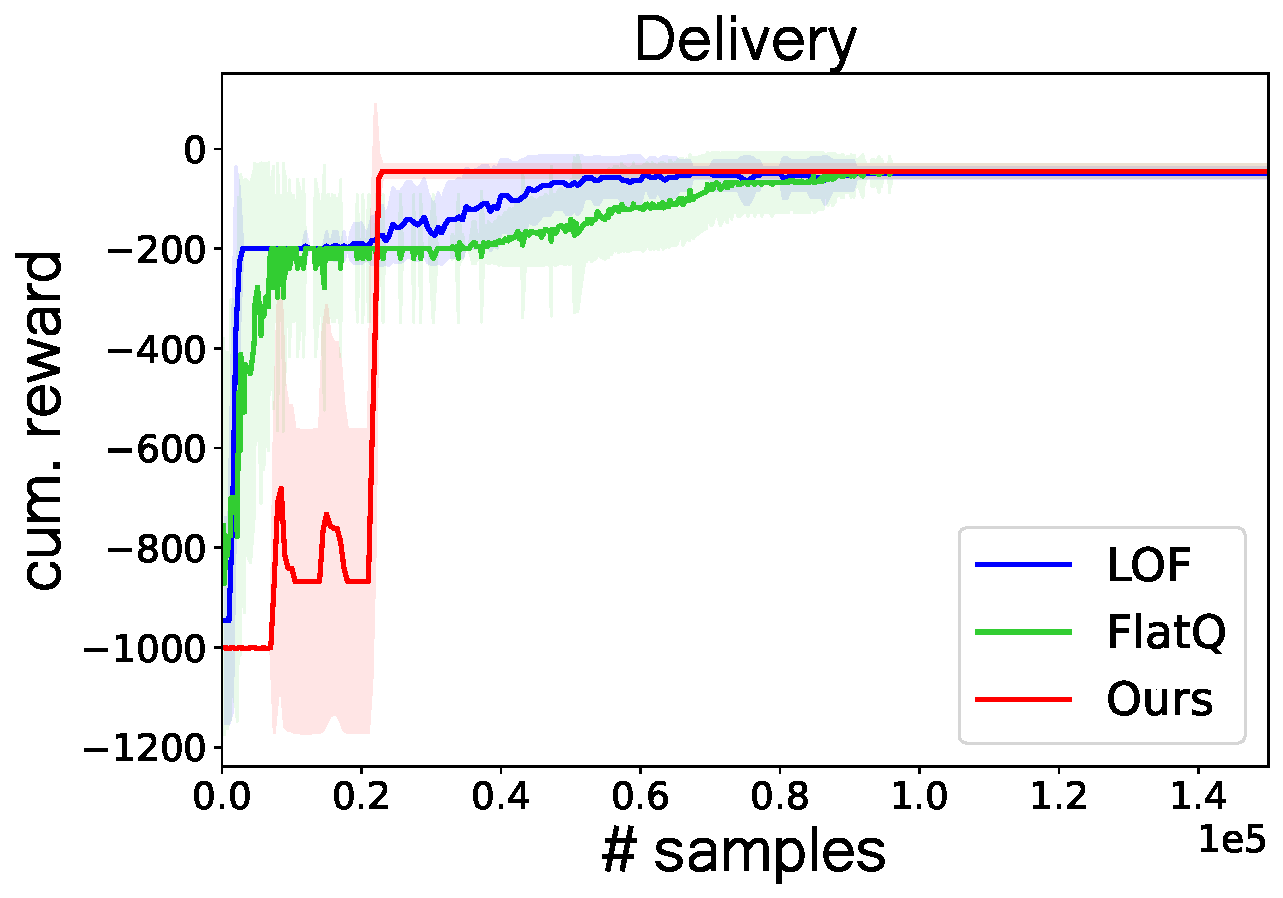
\includegraphics[scale=0.28]{figures/chapter3/results/delivery_learning.pdf}  
    % \subcaption{}
    % \label{fig:results1}
  \end{subfigure}
  \hfill
   \begin{subfigure}[t]{0.5\textwidth}
    \centering
    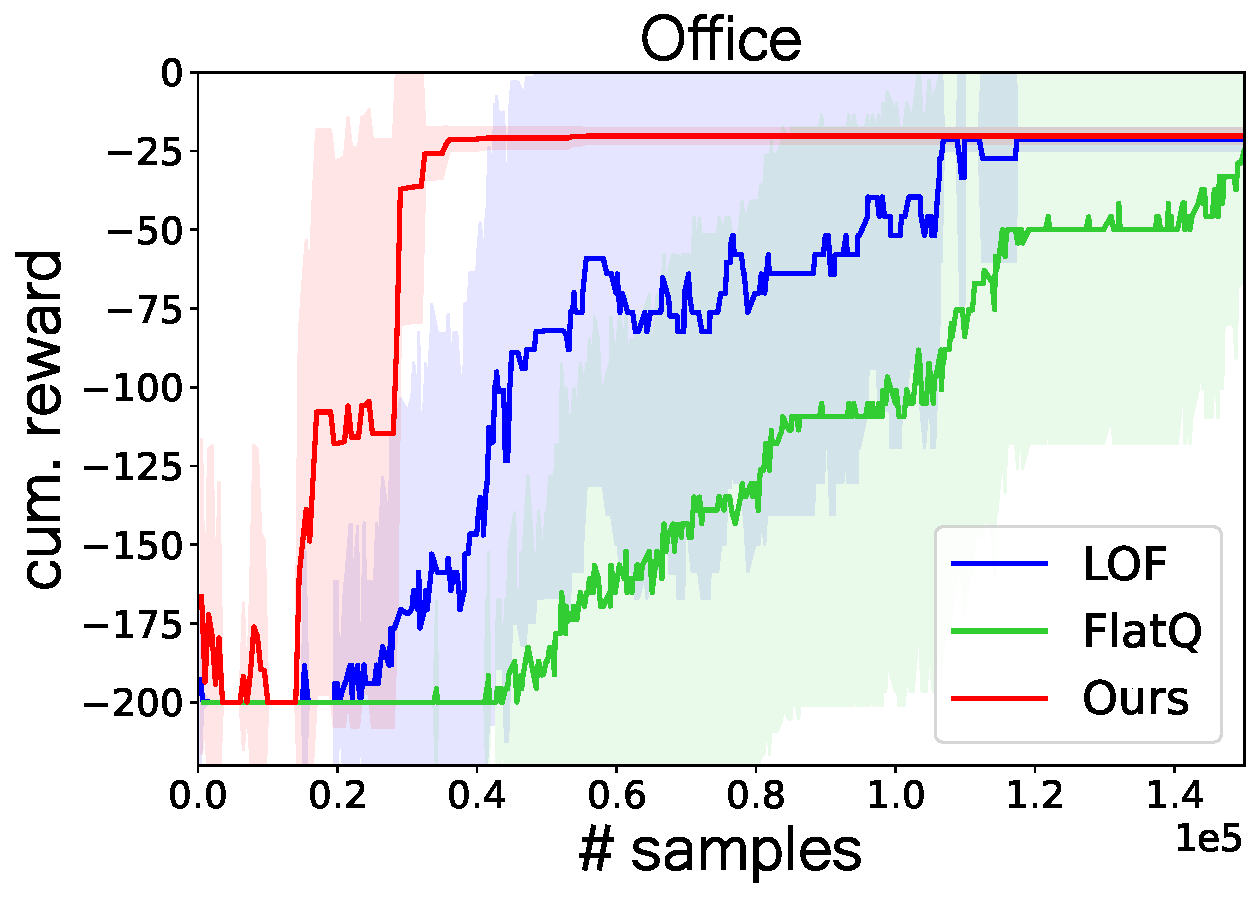
\includegraphics[scale=0.28]{figures/chapter3/results/office_learning.pdf}  
    % \subcaption{}
    % \label{fig:results2}
  \end{subfigure}
   \begin{subfigure}[b]{0.5\textwidth}
    \centering
    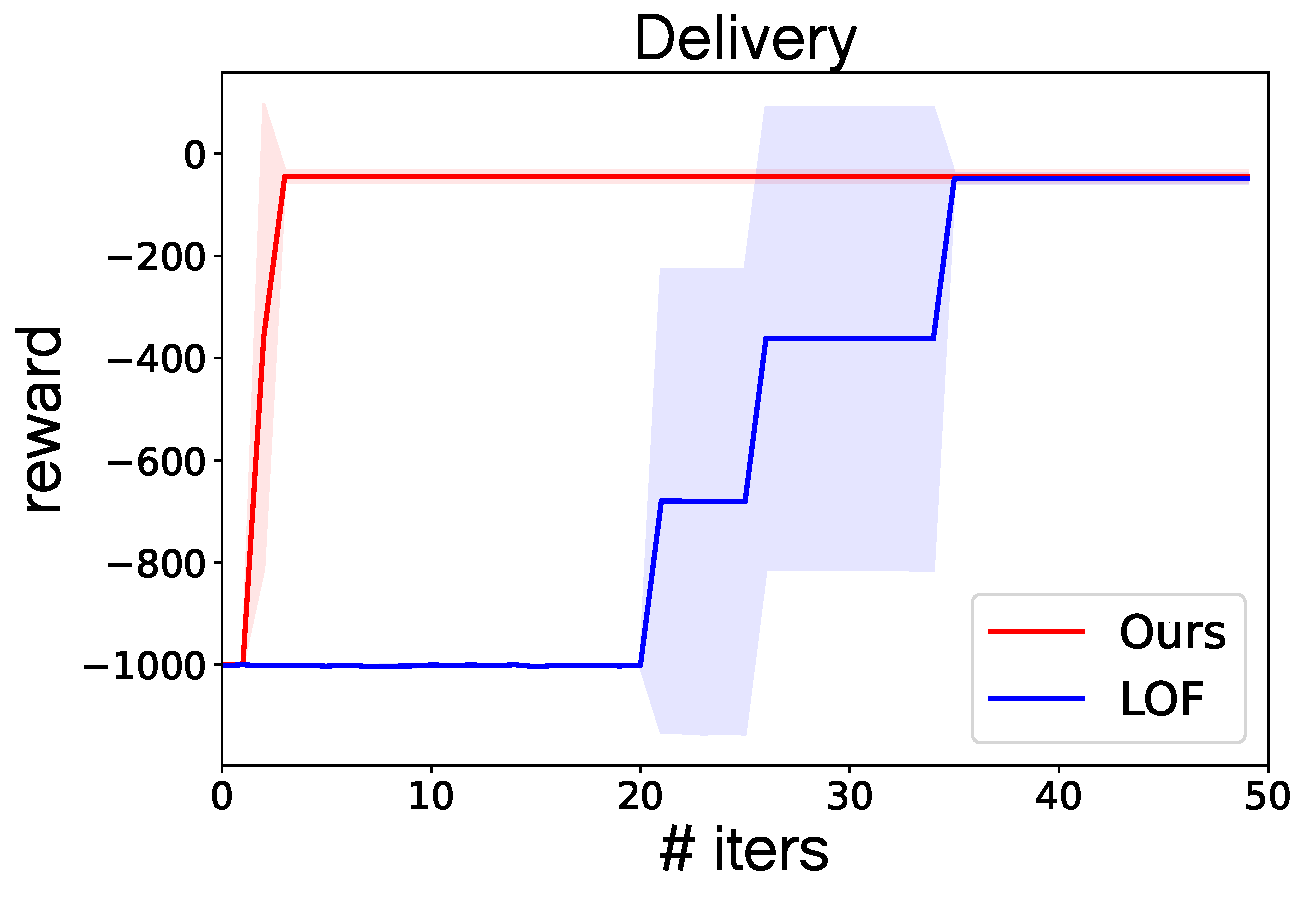
\includegraphics[scale=0.28]{figures/chapter3/results/readapt_delivery.pdf}  
    % \subcaption{}
    % \label{fig:results3}
  \end{subfigure}
  \hfill
   \begin{subfigure}[b]{0.5\textwidth}
    \centering
    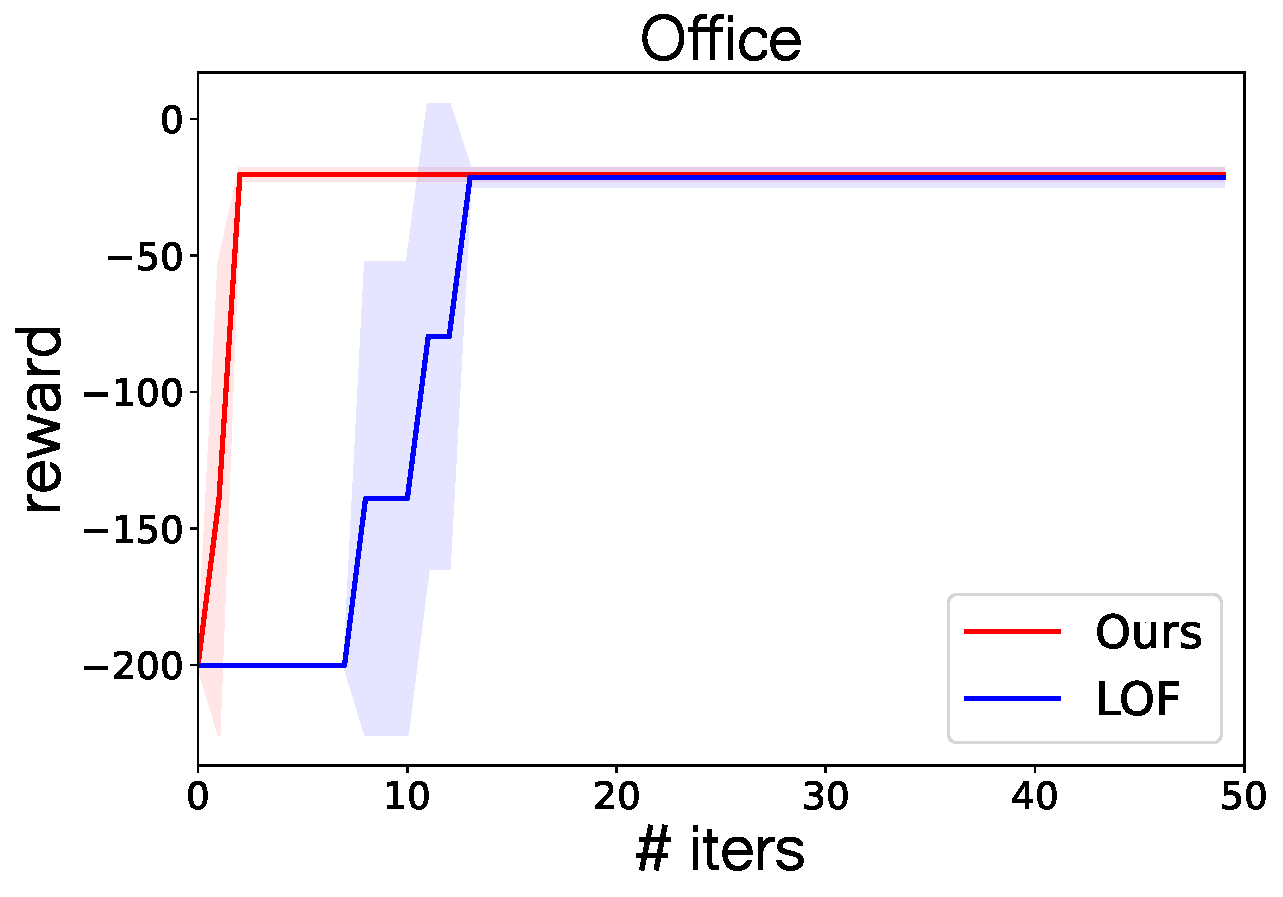
\includegraphics[scale=0.28]{figures/chapter3/results/readapt_office.pdf}  
    % \subcaption{}
    % \label{fig:results4}
  \end{subfigure}
  \caption{Experimental results for learning (Delivery, top-left and Office, bottom-left) and compositionality (Delivery, top-right and Office, bottom-right). Results show the average performance and standard deviation over the three tasks and 5 seeds per task.}
  \label{fig:exp_results}
\end{figure*}
We test SF-FSA-VI in two complex discrete environments. At test time, we change the reward to $-1$ for every timestep and use the cumulative reward as the performance metric. We report two types of results. First, we are interested in observing the performance of the derived optimal policy, in Equation~\eqref{eq:hl-policy}, during the learning phase. For this, we fully retrain the high-level policy (lines 2-6 in Algorithm~\ref{alg:online}) every several interactions with the environment as $\Pi_\text{CCS}$ is being learned. Second, once the base behaviors are learned (this is once a complete $\Pi_\text{CCS}$ has been computed), we measure how many planning iterations SF-FSA-VI needs to converge to an optimal solution for different task specifications. In both cases, we compare against existing baselines.

\subsubsection{Environments and tasks} We use the Delivery domain~\citep{Araki2021} and a modified version of the Office domain~\citep{Icarte2022} as testbeds for our algorithm. Both environments are depicted in Figure~\ref{fig:domains} and present a propositional vocabulary that is rich enough to build complex tasks. In the Delivery domain there is a single low-level state associated with each of the propositional symbols, implying that ${\cE=\cP=\{A,B,C, H\}}$. The feature vectors are consistent with our design choice. For terminal transitions, they correspond to their one-hot encodings of the terminal states. There exist obstacle states (in black) for which, upon entering,  the feature vector is $\boldsymbol{\phi}(s,a,s')=\mathbf{-1000}\in\real^4$. This transforms in a large negative reward when multiplied with a corresponding weight vector $\w\in\real^{4}$. For regular grid cells (in white) $\boldsymbol{\phi}(s,a,s')=\mathbf{0}\in\real^{4}$. The Office domain is more complex since there are three propositional symbols $\cP=\{\text{\coffee}, \text{\mail}, o\}$ which can be satisfied at different locations, namely $\cE=\{\text{\coffee}^1, \text{\coffee}^2, \text{\mail}^1, \text{\mail}^1, o^1, o^2\}$. Here, there are no obstacle states and $\boldsymbol{\phi}(s,a,s')=\mathbf{0}\in\real^6$ for non-terminal transitions.

For each of the environments we define three different tasks: sequential, disjunction and composite (all described in the Supplementary Material). The sequential task is meant to show how our algorithm can indeed be effectively used to plan over long horizons, when the other two tasks show the ability of our method to optimally compose the base (sub)policies in complex settings. In natural language, the tasks in the Delivery domain correspond to: "go to $A$, then $B$, then $C$ and finally $H$"  (sequential), "go to $A$ or $B$, then $C$ and finally $H$" (disjunction) and "go to $A$ and $B$ in any order, then $B$, then $C$ and finally $H$" (composite). The agent has to complete the tasks by avoiding obstacles. The counterpart of these tasks in the Office environment are: "get a coffee, then pick up mail and then go to an office" (sequential), "get a coffee or mail, and then go to an office" (disjunction) and "get a coffee and mail in any order, and then go to an office" (composite). 
Our agent never learns how to solve these tasks, but rather learns the set of (sub)policies that constitutes the CCS. At test time, we provide the agent with the FSA task specification, extract a high-level optimal policy and test its performance on solving the task.

\subsubsection{Baselines} In the literature, we find the most similar approach to ours in the Logical Options Framework (LOF) ~\citep{Araki2021}. We thus use LOF and flat Q-learning on the product MDP as baselines. LOF trains one option per exit state, which are trained simultaneously using intra-option learning, and then uses a high-level value iteration algorithm to train a meta-policy that decides which option to execute in each of the MDP states. On the other hand, the latter learns the action value function in the flat product MDP, from which it extracts the policy. Under certain conditions, flat Q-learning converges to the optimal value function but, especially for longer tasks, it may take a large number of samples. Additionally, it is trained for a specific task, so it is not able to generalize to other task specifications. For LOF, we followed the implementation details prescribed by the authors. 

\subsection{Results}
\subsubsection{Learning} Empirical results for learning are shown in Figure~\ref{fig:exp_results} (top-left and bottom-left). The plots reflect how the different methods (ours, LOF and flat Q-learning) perform at solving an FSA task specification during the learning phase. In the case of SF-FSA-VI and LOF, the learning phase corresponds to obtaining the low level (sub)policies for $\Pi_\text{CCS}$ and the options, while for . Results are averaged over the three tasks (sequential, disjunction and composite) previously described for each environment. Each data point in the plots represent the cumulative reward obtained by a fully retrained policy with the current status of $\Pi_\text{CCS}$ and options. In both environments, SF-FSA-VI is the first to reach optimal performance. There exist, however, some differences between LOF and SF-FSA-VI. LOF trains all options simultaneously with intra-option learning. This means that, every transition $(s_t, a_t, s_{t+1})$ is used to update all options' value functions and policies. The learning of a $\Pi_\text{CCS}$, on the other hand, is done sequentially. A fixed sample budget per (sub)policy is set prior to learning, which can be seen as a hyperparameter. We use a total of $8\cdot 10^3$ samples per (sub)policy in both environments. A experience replay buffer is used to speed up the learning of the policy basis $\Pi_\text{CCS}$. Both options and the SF representation of (sub)policies are learned using Q-learning. Due to the incremental nature, at the beginning of the learning process there might be not enough policies in the basis $\Pi_\text{CCS}$ to construct a feasible solution. This is clearly observed in the Delivery domain (Figure~\ref{fig:exp_results}, top left), where at the early stages of the interaction, SF-FSA-VI achieves very low cumulative reward due to failing at delivering a solution. It is not until when there are enough (sub)policies in the basis that Algorithm~\ref{alg:online} attains a policy that solves the problem, which eventually converges to an optimal policy. Similarly, LOF converges to an optimal policy albeit it takes slightly longer to learn. In the more complex Office environment, results follow the same pattern. However, this environment breaks one of the of LOF requirements for optimality: to have a single exit state associated with each propositional predicate. In this problem, for each predicate there exist two exit states that can satisfy them. This makes LOF prone to converge to suboptimal solutions when SF-FSA-VI attains optimality. This is the case for the composite task, where LOF is short-sighted and returns a longer path (in red, Figure~\ref{fig:office_domain}) in contrast to ours that retrieves the optimal solution (in green, Figure~\ref{fig:office_domain}). This means that SF-FSA-VI is more flexible in the task specification. In this environment, our algorithm also converges faster with a more obvious gap with respect to LOF. In any case, learning (sub)policies or options is faster than learning directly on the flat product MDP, as flat Q-learning takes the longest to converge.
\subsubsection{Planning} Figure~\ref{fig:exp_results} top-right and bottom-right show how fast SF-FSA-VI and LOF can plan for an optimal solution. Results are again averaged for the three tasks for each environment. Here, a complete policy basis $\Pi_\text{CCS}$ has been previously computed, as well as the option's optimal policies.  In LOF, the cost of each iteration of value iteration is $\lvert\cU\rvert\times\lvert\cS\rvert\times \lvert\cK\rvert$, where $\cK$ is the set of options, while for the Algorithm~\ref{alg:online} we propose it is $\lvert\cU\rvert\times\lvert\cE\rvert\times\lvert\Pi_\text{CCS}\rvert$. By definition, the number of options is equivalent to the number of exit states $\lvert\cK\rvert=\lvert\cE\rvert$, so a single iteration of SF-FSA-VI is more efficient than LOF whenever $\lvert\Pi_\text{CCS}\rvert \ll \lvert\cS\rvert$. In our experiments, the sizes of the CCS are $15$ and $12$ for the Delivery and Office domains, respectively, while the sizes of the state spaces are of $225$ and $121$. Therefore, since our algorithm needs fewer, shorter iterations during planning, it outperforms LOF in terms of planning speed in both domains when composing the global solution. This can be observed in the plots for both environments. 

\subsubsection{Policy basis over options} In deterministic environments, it is sufficient to learn the (sub)policies associated with the extrema weights (i.e. those (sub)policies that reach each of the exit states individually) to find a globally optimal policy via planning. In such cases, it may not be necessary to learn a full CCS. That is why, approaches that use the options framework such as LOF traditionally define one option per subgoal. However, there are scenarios, in which these approaches will not find optimal policy. This is the case for most stochastic environments. For example, consider the very simple domain of Double Slit in and the FSA task specification in Figure~\ref{fig:double_slit}. In this environment, there are two exit states $\cE=\{{\color{blue} \text{blue}}, {\color{red}\text{red}}\}$. The agent starts in the leftmost column and middle row. At every timestep, the agent chooses an action amongst $\{\text{UP}, \text{RIGHT}, \text{DOWN}\}$ and is pushed one column to the right in addition to moving in the chosen direction, except in the last column. If the agent chooses RIGHT, he moves an extra column to the right. At every timestep there is a random wind that can blow the agent away up to three positions in the vertical direction. The FSA task specification represents a task in which the agent is indifferent between achieving either of the goal states. Since the RIGHT action brings the agent closer to both goals, the optimal behavior in this case is to commit to either goal as late as possible. In this setting, methods that use one policy per sub-goal, such as LOF, train two policies to reach both goals. This means that the agent has to commit to one of the goals from the very beginning, which hurts the performance as it has to make up for the consequences of the random noise. On the other hand, the CCS used by SF-FSA-VI will contain an additional policy that is indifferent between two goals. This leads to a performance gap as our approach achieves an average accumulated reward of $-19.7\pm3.65$ and LOF $-22.70\pm 5.72$.

% \begin{figure}[!htb]
%   \centering
%   \begin{subfigure}[t]{0.23\textwidth}
%     \centering
%     \begin{tikzpicture}[scale=0.54]

    % Outer box
    \draw[step=0.5cm,lightgray] (0,0) grid (8, 6);
    \draw[ultra thick] (0,0) rectangle (8,6);

    % agent
    \node at (0.3, 2.8) {\miniagent};
    % \draw[ultra thick, ->, >=stealth, draw=blue!70!white] (2.5,1.9) -- (2.5,2.5) -- (1.5,2.5) -- (1.5,3.5) -- (2.5,3.5) -- (2.5,5.5) -- (1.5,5.5) -- (1.5,6.5) -- (2.5,6.5) -- (2.5,7.5) -- (3.5,7.5) -- (3.5,6.8);
    % \draw[ultra thick, ->, >=stealth, draw=blue!70!white] (3.8,6.5) -- (4.3,6.5) -- (4.3,4.8);
    \draw[fill=blue] (7.5,5.5) --  (7.5,6) -- (8,6) -- (8,5.5) -- cycle;
    % Outer box
    \draw[fill=red]  (7.5,0) --  (7.5,0.5) -- (8,0.5) -- (8,0) -- cycle;

    % \node[color=white] at (7.5,5.5) {$\text{G}_1$};
    % \node[color=white] at (7.5,0.5) {$\text{G}_2$};

\end{tikzpicture}

%   \end{subfigure}
%   \hfill
%   \begin{subfigure}[t]{0.23\textwidth}
%     \centering
%     \begin{tikzpicture}[node distance=cm,on grid,every initial by arrow/.style={ultra thick,->, >=stealth}]
    \node[thick,state,initial above] (u_0) at (0,0) {$u_0$};
    % \node[circle,draw=black,minimum size=0.26cm,inner sep=0pt,fill=black] (t1) at (2,0)  {};
    % \node[circle,draw=black,minimum size=0.26cm,inner sep=0pt,fill=black] (t2) at (2,-1.8)  {};
    \node[circle,draw=black,minimum size=0.26cm,inner sep=0pt,fill=black] (t1) at (-0.5,-1.5)  {};
    \node[circle,draw=black,minimum size=0.26cm,inner sep=0pt,fill=black] (t2) at (0.5,-1.5)  {};
    \node[text width=1cm ] at (-0.7,-1.5) {$u_1$};
    \node[text width=1cm ] at (1.2,-1.5) {$u_2$};
    \path[thick,->, >=stealth] (u_0) edge node [left] {\color{blue} blue} (t1);
    \path[thick,->, >=stealth] (u_0) edge node [right] {\color{red} red} (t2);
    %\path[ultra thick,->, >=stealth] (q_0) edge [loop left] node {$\tuple{\neg \text{\coffee},0}$} ();
    % \path[ultra thick,->, >=stealth] (q_0) edge node [above] {$\tuple{\text{\decoration},0}$} (t1);
    %\path[ultra thick,->, >=stealth] (q_1) edge [loop left] node {$\tuple{\neg o,0}$} ();
    % \path[ultra thick,->, >=stealth] (q_1) edge node [above] {$\tuple{\text{\decoration},0}$} (t2);
    %\path[ultra thick,->, >=stealth] (u_1) edge node [above]{$o$} (t3);
\end{tikzpicture}
%   \end{subfigure}
%   \caption{Double Slit environment (left) and FSA task specification to reach either goal locations {\color{blue}blue} or {\color{red}red}.}
%  \label{fig:double_slit}
% \end{figure} 

\section{Related Work}
One of the key distinctions in our research compared to prior studies is the optimality of the final solution. As noted by \textit{Dietterich2000}, hierarchical methods usually have the capability to achieve hierarchical, recursive, or global optimality. The challenge that often arises when sub-task policies are trained in isolation is that the combination of these locally optimal policies does not lead to a globally optimal policy but a recursively \textit{Dayan1992} or hierarchically optimal policy \textit{Sutton1999, mann2015approximate, Araki2021}.  To tackle this challenge, our approach relies on acquiring a set of low-level policies for each sub-task and employing planning to identify the optimal combination of low-level policies when solving a particular task. By learning the CCS with OLS \textit{roijers2014linear} in combination with high-level planning our approach ensures that globally optimal policy is found. In this regard, the work of \textit{Alegre2022} is of particular interest as it was the first work that used OLS and successor features \textit{Barreto2017} for optimal policy transfer learning. However, this method has only applied in a setting with Markovian reward function and has not been used with non-Markovian task specifications or high-level planning. 

On the other hand, many recent approaches proposed to use high-level task specifications in the form of LTL~\citep{Icarte2018b, kuo2020encoding, Vaezipoor2021, Jothimurugan2021}, or similar formal language specifications~\citep{ToroIcarte2019,Camacho2019, Araki2021, Icarte2022} to learn policies. However, the majority of the methods in this area are designed for single-task solutions, with only several focusing on acquiring a set of policies that is capable of addressing multiple tasks \textit{Icarte2018b, Leon2020, kuo2020encoding, Araki2021, Vaezipoor2021}. But, in contrast to our approach, they do not guarantee optimality of the solution.

From these works, our approach is the most similar to the Logical Options Framework \textit{Araki2021}. The main difference is that LOF trains a single policy for each sub-goal, resulting in a set of learned policies that is either smaller than or equal to the set acquired through SF-FSA-VI. While employing one policy per sub-goal proves sufficient for obtaining a globally optimal policy through planning in deterministic environments~\citep{Wen2020}, this may not hold true in stochastic environments, as our experiments demonstrate. In such instances, the policies generated by LOF are hierarchically optimal but fall short of global optimality.


Two notable examples from aforementioned works on multi-task learning with formal language specifications are the works of \textit{Icarte2018b} and \textit{Vaezipoor2021}. The former struggles with generalizing to unseen tasks, because it uses LTL progression to determine which sub-tasks need to be learned to solve given tasks. The Q-functions that are subsequently learned for each LTL sub-task will therefore not be useful for a new task if its sub-tasks were not part of the training set. Such limitation does not apply to the latter as it instead encodes the remaining LTL task specification using a neural network and conditions the policy on this LTL embedding. While this approach may be more adaptable to tasks with numerous propositions or sub-goals, it risks generating sub-optimal policies as it relies solely on the neural network to select the next proposition to achieve, without incorporating planning. Additionally, since the planning is implicitly done by the neural network, the policy is less interpretable than when explicit planning is used.

The method we propose can be viewed as a method for composing value functions through successor features, akin to previously proposed approaches for composition of value functions and policies ~\citep{Niekerk2019, Barreto2019, NangueTasse2020, Infante2022}. In the work of ~\citep{Infante2022}, which is the closest to our work, the authors propose to learn a basis of value functions that can be combined to form an optimal policy. However, unlike SF-FSA-VI, their approach only works in a restricted class of linearly-solvable MDPs. Lastly, since our approach uses the values of exit states for planning it is also related to planning with exit profiles \textit{Wen2020}. The CCS that we propose to use as a policy basis in our work can be seen as a collection of policies that are optimal for all possible exit profiles.

\section{Discussion and Conclusion}

In this work, we address the problem of finding optimal behavior for new non-Markovian goal specifications in known environments. To do so, we introduce a novel approach that uses successor features to learn a policy basis, that can subsequently be used to solve any unseen task specified by an FSA with the set of given predicates $\cP$ by planning. SF-FSA-VI is the first that can provably generalize to such new task specification without sacrificing optimality in both deterministic and stochastic environments.

The experiments show that SF-FSA-VI offers several advantages over previous methods. First, due to the use of SF, it allows for faster composition of the high-level value function since it drastically reduces the number of states to plan on. Secondly, thanks to using a CCS over a set of options SF-FSA-VI achieves optimality even in stochastic environments (as shown in the Double Slit example). Lastly, we do not require that there exists a single exit state per predicate which permits more flexible task specification while at the same time allowing deployment in more complex environments. 

A limitation of our approach could be the need to construct a full CCS if one wants to attain global optimality. While the construction of CCS is not timecomsuming for environments with several exit states presented in our work, the computation cost of finding the full CCS could become too large for environments with many exit states. In such case one could instead learn a partial CCS at the cost of a bounded decrease in performance \textit{Alegre2022} or consider splitting the environment into smaller parts with fewer exit states. While our experiments only considered discrete environments, SF-FSA-VI should also be applicable in continuous environments with minor adjustments. These include: using an contiguous set of states instead of a single exit state and using reward shaping to facilitate learning in sparse reward setting.
% \chapter{Conclusion}
% \input{chapters/conclusion}

\bibliographystyle{plainnat}
\bibliography{bibliography}

\appendix
\section{Proof Theorem~\ref{theo:almdps}}
\label{proof:theo_almdps}
\subsection{Preliminaries}
We introduce the notation:
\begin{itemize}
    \item $\mathds{1}$ denotes an all-ones vector of length $\lvert\cS\rvert$.
    \item $\indicator{p}$ is the indicator function that takes $1$ when predicate $p$ is true and $0$ otherwise.
\end{itemize}

We assumme an underlying continuing LMDP $\cL=\langle\cS,\cP,\cR\rangle$ where $\cS$ represents the state space, $\cP$ the passive dynamics and $\cR$ the reward function. Similarly to [Section B.1] in~\cite{Wan2021}, we also assume there exists a set-valued process $\{X_t\}$ where $X_t$ is a non-empty subset defined as ${X_t = \{ (s) : s\;\text{component of $v$ was updated at timestep $t$} \}}$.

We recall that the TD updates in the asynchronous case are 
\begin{align}
\widehat{v}_{t+1}(s) &\gets \widehat{v}_t(s) + \alpha_t(s) \delta_t(s) \indicator{s\in X_t},\label{eq:updatev}\\
\widehat{\rho}_{t+1} &\gets \widehat{\rho}_t + \lambda \sum_s \alpha_t(s) \delta_t(s) \indicator{s\in X_t}.\label{eq:updaterho}
\end{align}
The indicator $\indicator{s\in X_t}$ specifies whether the value of state $s$ updates at timestep $t$. The TD error for state $s$ is
\begin{align*}
\delta_t(s) %&= r_t(s) - \widehat{\rho}_t - \frac 1 \eta \log \frac {\widehat{\pi}_t(s_{t+1}|s_t)} {\cP(s_{t+1}|s_t)} + \widehat{v}_t(s_{t+1}) - \widehat{v}_t(s_t)\\
 &= r_t(s) - \widehat{\rho}_t + \frac 1 \eta \log \sum_{s'\in\cS} \cP(s'|s) e^{\eta \widehat{v}_t(s')} - \widehat{v}_t(s).
\end{align*}

We introduce a series of necessary assumptions for convergence. We adapt Assumptions B.1-B.5 in~\cite{Wan2021} to the case of LMDPs. Assumptions~\ref{ass:communicating} and~\ref{ass:uniqueness} are standard in average-reward settings, while Assumption~\ref{ass:stepsize1} is the standard Robbins-Monro conditions for step sizes. Assumptions~\ref{ass:stepsize2} and~\ref{ass:stepsize3} are introduced in the convergence argument of RVI Q-learning by~\citet{Borkar1998} and specify some requirements for the learning rates when asynchronous updates are performed. For more details we refer the reader to Section B.1 of~\cite{Wan2021}.
% \begin{assumption}
%  (Communicating assumption) The LMDP $\cL$ has a single communicating class, that is, each state in $\cL$ is accessible from every other state under some policy.
%  \label{ass:communicating}
% \end{assumption}

% NOT NEEDED since we have unichain

\begin{assumption}
 (Value function uniqueness) There exists a unique solution to $v$ in equation~\eqref{eq:boe_almdp} up to a constant shift.
  \label{ass:uniqueness}
\end{assumption}
\begin{assumption} (Stepsize assumption)
    \begin{equation*}
        \alpha_t > 0,\;\sum_{t=0}^{\infty} \alpha_t = \infty,\;\sum_{t=0}^{\infty} \alpha_t^2 < \infty.
    \end{equation*}
      \label{ass:stepsize1}
\end{assumption}
\begin{assumption}
    (Asynchronous Stepsize 1) Let $[\cdot]$ denote the integer part of $(\cdot)$, for $x\in(0, 1)$
    \begin{equation*}
        \sup_i \frac{\alpha_{[xi]}}{\alpha_i} < \infty
    \end{equation*}
    and
    \begin{equation*}
        \frac{\sum_{j=0}^{[yi]}\alpha_j}{\sum_{j=0}^i\alpha_j}\rightarrow 1
    \end{equation*}
    \label{ass:stepsize2}
    uniformly in $y \in[x, 1]$.
\end{assumption}

\begin{assumption}
    (Asynchronous Stepsize 2) There exists $\Delta>0$ such that
    \begin{equation*}
        {\lim\inf}_{t\rightarrow\infty} \frac{\nu(t, s)}{t+1}\geq \Delta
    \end{equation*}
    almost surely, for all $s\in\cS$. Here $\nu(t, s)$ represents the visitation count for state $s$ up to timestep $t$. Furthermore, for all $x > 0$, let
    \begin{equation*}
        N(t, x) = \min \Big\{m > t: \sum_{i=t+1}^m \alpha_i \geq x \Big\}
    \end{equation*}
    \label{ass:stepsize3}
    the limit 
    \begin{equation*}
       \lim_{t\rightarrow\infty} \frac{\sum_{i=\nu(t, s)}^{\nu(N(t, x), s)} \alpha_i}{\sum_{i=\nu(t, s')}^{\nu(N(t, x), s')} \alpha_i}
    \end{equation*}
    exists for all $s, s'\in\cS$.
\end{assumption}

Under the communication assumption, the system
\begin{align}
    v(s) &= \cR(s) - \rho + \frac{1}{\eta} \log \sum {\cP(s'\lvert s) e^{\eta v(s')}},\;\;\forall s\in\cS, \\
    \rho - \hat\rho_0 &= \lambda \Big(\sum_s v(s) - \sum_s\hat v_0(s)\Big),
\end{align}
has a unique solution for $v$ which we denote as $v_\infty$, where $\rho$ is the optimal gain.

At each timestep the increment to $\hat\rho_t$ is $\lambda$ times the increment to $\hat v_t$, and thus, to $\sum_s \hat v_t(s)$. The cumulative increment at $t$ can be expressed as
\begin{align}
     \hat\rho_t - \hat\rho_0 &= \lambda \sum_{i=0}^{t-1}\sum_s \alpha_i(s)\delta_i(s) \indicator{s\in X_t}\nonumber\\
                   &= \lambda \Big(\sum_s\hat v_t(s) - \sum_s\hat v_0 (s)\Big)\nonumber \\
    \implies \hat\rho_t &= \lambda \sum_s \hat v_t(s) - \lambda\sum_s \hat v_0 (s) + \hat\rho_0 \\
    &= \lambda\sum_s \hat v_t(s) - c, \label{eq:cum_rho}\\
    \text{where}\;c &= \lambda \sum_s \hat v_0(s) - \hat\rho_0.
\end{align}

If we replace~\ref{eq:cum_rho} in~\ref{eq:updatev}, we obtain
\begin{equation}
    \widehat{v}_{t+1}(s) \gets \widehat{v}_t(s) + \alpha_t(s) \widetilde\delta_t(s)  \mathbb{I}\{s\in X_t\},~~\forall{s\in\cS},
    \label{eq:td_asynchronous_full}
\end{equation}
where
\begin{equation}
    \widetilde\delta_t(s) = r_t(s) + c - \lambda\sum_s \hat v_t(s) - \frac 1 \eta \log \sum_{s'\in\cS} \cP(s'|s) e^{\eta \widehat{v}_t(s')} - \widehat{v}_t(s).
\end{equation}

This can be interpreted as the TD error of an alternative LMDP $\widetilde\cL=\langle\cS,\cP,\widetilde\cR\rangle$ in which the reward is defined as $\widetilde\cR(s) = \cR(s) + c$ and the gain estimate equals $\lambda \sum_{s\in\cS} \widehat{v}_t(s)$.
%$\lambda \sum_{s'\in\cS} \widehat{v}_t(s)$.
The gain of $\widetilde\cL$ satisfies 
\begin{equation}
    \widetilde\rho = \rho + c.
    \label{eq:alternative_reward}
\end{equation}

The former expression, combined with~\eqref{eq:cum_rho} gives
\begin{equation}
    \widetilde\rho = \lambda \sum_s v_\infty.
    \label{eq:extended_rho}
\end{equation}
It is easy to verify that $v_\infty$ is not only the solution for the original LMDP $\cL$, but also for the alternative LMDP $\widetilde\cL$,
\begin{align*}
     v_\infty(s) &= \cR(s) - \rho + \frac{1}{\eta} \log \sum_{s'} {\cP(s'\lvert s) e^{\eta v_\infty(s')}}\;\;\forall s\in\cS\\
     &= \cR(s) - \widetilde\rho + c + \frac{1}{\eta} \log \sum_{s'} {\cP(s'\lvert s) e^{\eta v_\infty(s')}}\;\;\forall s\in\cS\;(\text{by}~\eqref{eq:alternative_reward})  \\
      &= \widetilde\cR(s) - \widetilde\rho + \frac{1}{\eta} \log \sum_{s'} {\cP(s'\lvert s) e^{\eta v_\infty(s')}}\;\;\forall s\in\cS.
\end{align*}

Now consider $\hat\rho_t$. If we can prove that $\hat v_t\rightarrow v_\infty$ then by~\eqref{eq:cum_rho} we have $\hat\rho_t\rightarrow\lambda\sum v_\infty - c$. By~\eqref{eq:extended_rho}, we know that $\lambda\sum v_\infty = \widetilde\rho$, then we have $\hat\rho_t\rightarrow\widetilde\rho-c$. Using~\eqref{eq:alternative_reward}, we get 
\begin{equation*}
    \hat\rho_t\rightarrow\rho\;\text{almost surely as}\;t\rightarrow\infty.
\end{equation*}

The idea is to prove the convergence of differential soft TD-learning for the alternative LMDP $\widetilde\cL$, which is the same solution as for the original LMDP $\cL$.

We adapt Theorem B.2 in~\cite{Wan2021}.

\begin{theorem} (Convergence of differential TD learning)
    For any $v_0\in\real^{\lvert\cS\rvert}$, let $r_t$, $X_t$, $\alpha_t$ be properly defined and consider the update rule
    \begin{equation}
        \widehat{v}_{t+1}(s) \gets \widehat{v}_t(s) + \alpha_t(s) \big( r_t(s) - \lambda\sum_s \hat v_t(s) - \frac 1 \eta \log \sum_{s'\in\cS} \cP(s'|s) e^{\eta \widehat{v}_t(s')} - \widehat{v}_t(s)\big)  \mathbb{I}\{s\in X_t\},
        \label{eq:td_update_theo}
    \end{equation}
    
    \begin{enumerate}
        \item Assumptions~\ref{ass:unichain} and~\ref{ass:uniqueness}-\ref{ass:stepsize3} hold.
        \item $f:\real^{\lvert\cS\rvert}\rightarrow\real$ is Lipschitz and there exists some $u>0$ such that $\forall c\in\real$ and $x\in\real^{\lvert\cS\rvert}$, $f(\mathds{1})=u$, $f(x + c\mathds{1})=f(x)+cu$ and $f(cx) = c f(x)$
    \end{enumerate}
    then $\hat v_t$ converges almost surely to $v_\infty$.
    \label{theo:our_theorem}
\end{theorem}

We observe that~\eqref{eq:td_update_theo} is in the same form of equationB.24 in~\cite{Wan2021} and equation7.1 in~\cite{Borkar2009}. Thus the results in Section 7.4 in~\cite{Borkar2009} and Theorem 3.2~\cite{Borkar1998} apply to show convergence of~\eqref{eq:td_update_theo}. Due to Assumptions~\ref{ass:stepsize2} and ~\ref{ass:stepsize3}, to show convergence of \eqref{eq:td_asynchronous_full} suffices to show convergence of the following synchronous update
\begin{equation}
    \widehat{v}_{t+1} \gets \widehat{v}_t + \alpha_t \pa{ T(\widehat{v}_t) - f(\widehat{v}_t) \mathds{1} - \widehat{v}_t + M_{t+1}}.
    \label{eq:synchronous}
\end{equation}

Here, $\hat v_t\in\real^{\lvert\cS\rvert}$ is interpreted as a vector, and the operator $T$ is a mapping $T:\real^d\rightarrow\real^d$ defined for each state $s$ as
\begin{equation*}
    T(v)(s) = \cR(s) + \frac 1 \eta \log \sum_{s'\in\cS} \cP(s'|s) e^{ \eta v(s') }.
\end{equation*}
We also define the following operators, 
\begin{align*}
    T^1(v) &= T(v) - \rho\mathds{1} \\
    T^2(v) &= T(v) - f(v)\mathds{1} =  T^1(v) + (\rho - f(v))\mathds{1}.
\end{align*}

The function $f$ is given by $f(v) = \lambda\sum_s v(s)$, which satisfies condition 2 of Theorem~\ref{theo:our_theorem}. The error term $M_{t+1}=r_t-\cR$ is only needed in case the reward vector $r_t$ is sampled from a distribution with mean $\cR$; if reward is deterministic, $M_{t+1}$ can be omitted. If the reward is sampled from a distribution, it should be easy to show that $M_{t+1}$ has zero mean and bounded variance.

The operator $T$ is a non-expansion in the max-norm:
\begin{align*}
T(x)(s) - T(y)(s) &= \frac 1 \eta \log \sum_{s'} \cP(s'|s) e^{\eta x(s')} - \frac 1 \eta \log \sum_{s'} \cP(s'|s) e^{\eta y(s')}\\
 &= \frac 1 \eta \log \frac {\sum_{s'} \cP(s'|s) e^{\eta x(s')}} {\sum_{s'} \cP(s'|s) e^{\eta y(s')}}\\
 &\leq \frac 1 \eta \log \frac {\sum_{s'} \cP(s'|s) e^{\eta \pa{ y(s') + \infnorm{x-y} }}} {\sum_{s'} \cP(s'|s) e^{\eta y(s')}}\\
 &= \frac 1 \eta \log e^{\eta \infnorm{x-y} } \frac {\sum_{s'} \cP(s'|s) e^{\eta y(s')}} {\sum_{s'} \cP(s'|s) e^{\eta y(s')}}\\
 &= \infnorm{x - y}.
\end{align*}
Hence we have
\[
\infnorm{T(x)-T(y)} = \max_s |T(x)(s) - T(y)(s)| \leq \infnorm{x - y}.
\]

We also show the following property of $T$:
\begin{align*}
T(x + c\mathds{1})(s) &= \cR(s) + \frac 1 \eta \log \sum_{s'} \cP(s'|s) e^{\eta \pa{ x(s') + c }}\\
 &= \cR(s) + \frac 1 \eta \log e^{\eta c} \sum_{s'} \cP(s'|s) e^{\eta x(s')}\\
 &= \cR(s) + \frac 1 \eta \sum_{s'} \cP(s'|s) e^{\eta x(s')} + c\\
 &= T(x)(s) + c.
\end{align*}
Hence it follows that $T(x + c\mathds{1}) = T(x) + c\mathds{1}$.

We consider the following ordinary differential equations (ODEs),
\begin{align}
    \dot{y}_t &= T^1(y_t) - y_t \label{eq:ode1} \\
    \dot{x}_t &= T^2(x_t) - x_t \label{eq:ode2}.
\end{align}
Such equations are well-defined since both RHS's are Lipschitz thanks to the properties of $f$ and $T$.

\noindent We complete the proof as a succession of lemmas.

\begin{lemma}
    Let $\bar{y}$ be equilibrium point of the ODE defined in~\eqref{eq:ode1}. Then $\infnorm{y_t - \bar{y}}$ is non-increasing and $y_t\rightarrow y_\infty$ for some equilibrium point of \eqref{eq:ode2}.
\end{lemma}

\begin{proof}
    See Lemma 3.1 in~\cite{Abounadi2001}.
\end{proof} 

\begin{lemma}
    Equation~\eqref{eq:ode2} has a unique equilibrium at $v_\infty$.
\end{lemma}

\begin{proof}
    See Lemma 3.2 in~\cite{Abounadi2001}.
\end{proof}

\begin{lemma}
    Let $x_0=y_0$, then $x_t = y_t + z_t\mathds{1}$ satisfies the ODE $\dot{z}_t = -u z_t + (\rho - f(y_t))$.
\end{lemma}
\begin{proof}
    See Lemma 3.3 in~\cite{Abounadi2001}.
\end{proof} 

\begin{lemma}
    $v_\infty$ is the globally asymptotically stable equilibrium for~\eqref{eq:ode2}
\end{lemma}
\begin{proof}
    See Lemma B.4 in~\cite{Wan2021}.
\end{proof}  

\begin{lemma}
    Equation~\eqref{eq:synchronous} converges almost surely $\hat v_t$ to $v_\infty$ as $t\rightarrow\infty$.
\end{lemma} 
\begin{proof}
    See Lemma B.5 in~\cite{Wan2021} and Lemma 3.8 in~\cite{Abounadi2001}.
\end{proof}

Therefore, stability and convergence of equation~\eqref{eq:td_update_theo} is proved.

\backmatter 
\printindex



\end{document}


%NUMBER OF THE EXTERNAL PAGE EXCEPT IN THE FIRST PAGE OF EACH CAPITAL
\usepackage{fancyhdr}
\pagestyle{fancy}
\fancyfoot{}
\fancyfoot[RO]{\thepage}
\fancyfoot[LE]{\thepage}


%MULTIPLE INDEX
%In the preamble
\usepackage{multind}
\makeindex{authors}
%Introduction to form entries
\index{authors}{Einstein}
%Situation of the Index
\printindex{authors}{Author index}
%The \ usepakage {makeidx} \ makeindex \ printindex commands must be removed
%You need to exacute from the command line makeindex authors